\documentclass[journal=jcisd8,manuscript=suppinfo]{achemso}
\usepackage{lmodern}
\usepackage{setspace}
\usepackage[version=4]{mhchem}
\usepackage{amsmath,amssymb}
\usepackage{siunitx}
\DeclareSIUnit{\angstrom}{\text{\AA}}
\usepackage{booktabs}
\usepackage{longtable}
\usepackage{tabularx,array}
\usepackage{multirow}
\usepackage{graphicx}
\usepackage{enumitem}
\usepackage[section]{placeins}
\usepackage[english]{babel}
\IfFileExists{droidsans.sty}{\usepackage{droidsans}}{}
\usepackage{charter}
\usepackage[T1]{fontenc}
\usepackage[dvipsnames]{xcolor}
\newcommand{\tcb}[1]{{\textcolor{blue}{#1}}}
\usepackage[compact]{titlesec}
\usepackage{caption}
\captionsetup{font=small,labelfont=bf}
\usepackage{xr}
% Cross-references between the manuscript and the ESI (prefix M-).
\usepackage{etoolbox}
\makeatletter
\newcommand*{\addFileDependency}[1]{\typeout{(#1)}\@addtofilelist{#1}\IfFileExists{#1}{}{\typeout{No file #1.}}}
\makeatother
\newcommand*{\myexternaldocument}[2][]{\externaldocument[#1]{#2}\addFileDependency{#2.tex}\addFileDependency{#2.aux}}
\usepackage[hidelinks]{hyperref}
\myexternaldocument[M-]{Manuscript_V3}

\textheight=23cm
\textwidth=18cm
\oddsidemargin=-1.5cm
\evensidemargin=-1.5cm
\topmargin=-1.5cm
\setkeys{acs}{articletitle=true, maxauthors=0}
\graphicspath{{ESI_Figures_V3/}{MS_Figures_V3/}}
\setlist{nosep, leftmargin=*}
\newcommand{\ET}{E^{(2)}}
\newcommand{\BX}{BondX Studio}
\renewcommand{\thefigure}{S\arabic{figure}}
\renewcommand{\thetable}{S\arabic{table}}
\renewcommand{\theequation}{S\arabic{equation}}
\renewcommand{\thesection}{S\arabic{section}}
\renewcommand{\bibfont}{\footnotesize}
\setlength{\bibsep}{0pt}

\author{Soumyajit Karmakar}
\email{soumyajitkarmakar9991@kgpian.iitkgp.ac.in}
\author{Sabyashachi Mishra}
\email{mishra@chem.iitkgp.ac.in}
\affiliation[IIT Kharagpur]{Department of Chemistry, Indian Institute of Technology Kharagpur, Kharagpur 721302, India}
\title{BondX Studio: Screening Geometric Halogen Contacts with Force-Field-Consistent QM Models, NBO Analysis, and ALMO-EDA}

\SectionNumbersOn
\setcounter{tocdepth}{1}
\begin{document}
\begin{singlespace}
\maketitle
{\makeatletter\patchcmd{\l@section}{1.5em}{2.1em}{}{}\makeatother\tableofcontents}

\noindent The public project repository is \url{https://github.com/compchemsk/BondX-Studio}. The revised T1 implementation and analysis outputs used here were generated in a working-tree revision based on commit \texttt{971f1fa3bd1adcf74b2b6b078bd7ec408d4f1bc1}; the updated engine, tests, T1 tables, and figures accompany the revised manuscript source package and have not yet been pushed to the public repository. Energies are given in kcal\,mol$^{-1}$ throughout (1~kcal = 4.184~kJ).


%% =====================================================================
\section{Literature Counts}
\label{sec:counts}

{\sloppy We searched PubMed on 18 November 2026.\cite{PubMed2026} Query Q1 was \texttt{"halogen bond" OR "halogen bonding" OR "halogen bonds"}, and query Q2 was \texttt{(Q1) AND (protein OR drug OR ligand)}. Table~\ref{tab:counts} gives the records per year; PubMed can place one record in two years. The script \texttt{00\_pubmed\_xb\_counts.py} repeats the count. Since 2017, Q1 has returned between 222 and 290 records per year, and Q2 roughly one quarter of them.\par}

\begin{table}[!htbp]
\caption{PubMed records per year. Q2 is a subset of Q1. The 2026 count ends on 18 November.}
\label{tab:counts}
\centering\footnotesize
\begin{tabular}{@{}lrr|lrr|lrr@{}}
\toprule
Year & Q1 & Q2 & Year & Q1 & Q2 & Year & Q1 & Q2 \\
\midrule
2003 & 11 & 5   & 2011 & 95 & 27  & 2019 & 255 & 70 \\
2004 & 16 & 3   & 2012 & 116 & 33 & 2020 & 245 & 62 \\
2005 & 21 & 9   & 2013 & 153 & 30 & 2021 & 281 & 59 \\
2006 & 19 & 5   & 2014 & 161 & 27 & 2022 & 257 & 56 \\
2007 & 30 & 7   & 2015 & 200 & 42 & 2023 & 270 & 54 \\
2008 & 48 & 11  & 2016 & 188 & 46 & 2024 & 232 & 54 \\
2009 & 58 & 11  & 2017 & 255 & 55 & 2025 & 290 & 86 \\
2010 & 61 & 12  & 2018 & 222 & 65 & 2026 & 280 & 85 \\
\bottomrule
\end{tabular}
\end{table}

%% =====================================================================
\section{Assumptions of Every Tier}
\label{sec:assume}

Each tier page of \BX{} shows the text below. The list uses the default parameters and changes with every parameter change.

% ---- table from tables/tab_assumptions.tex (generated) ----
\paragraph{Tier T0, structure input.}
\begin{itemize}[nosep,leftmargin=*]
\item The first MODEL of a multi-model file defines the atoms. Later models serve as trajectory frames.
\item For alternate locations, the first conformer (A, 1, or blank) is kept.
\item Virtual sites are removed on reading. Examples are the $\sigma$-hole extra point (EP) of a halogen, LP sites, and TIP4P M sites. DCD and XYZ frames with these sites are mapped onto the remaining atoms.
\item Bonds come from distances: d $<$ r\_cov(1) + r\_cov(2) + 0.45 \AA{}. Links between residues are limited to peptide, disulfide, and phosphodiester bonds.
\item Element symbols come from columns 77--78. Atom names supply missing element symbols.
\item Residues are classed as protein, nucleic acid, water, ion (single atom), or ligand (all other residues).
\end{itemize}
\paragraph{Tier T1, geometry.}
\begin{itemize}[nosep,leftmargin=*]
\item Donors: C-bound Cl, Br, and I atoms of ligands and modified residues.
\item A halogen bond needs d(X$\cdots$Y) $\le$ the pair cut-off and 140$^\circ$ $\le$ $\theta_1$ $\le$ 180$^\circ$.
\item Acceptors: protein N/O/S, nucleic-acid N/O, and aromatic rings (Phe, Tyr, Trp, and nucleobases) with $\alpha$ $\le$ 60$^\circ$.
\item R = d / (r\_X + r\_Y) with Bondi radii. An aromatic centroid has r = 1.77 \AA{}.
\item G = [g\_d $\cdot$ g\_$\theta$ $\cdot$ ($\frac12$ + $\frac12$ g$_2$)]\^{}$\frac13$. g\_d = 1 at R $\le$ 0.85. For atom acceptors, g$_2$ is a Gaussian centred at $\theta_2$ = 180$^\circ$ (sp), 120$^\circ$ (sp$^2$), or 109.5$^\circ$ (sp³), with common width 40$^\circ$; undetermined environments use the sp$^2$ value. Ring acceptors use the ring-normal term. Contacts with R $<$ 0.8 are flagged as short.
\item Poor Lewis bases are kept with a flag: N atoms with a delocalized lone pair (backbone amide N, Asn ND2, Gln NE2, and Trp NE1) and protonated N atoms (Lys NZ, Arg NE/NH1/NH2). Such contacts need the NBO step and a check for N--H$\cdots$X hydrogen bonds.
\item The iodine cut-offs are inherited from the earlier hIYD study. The Br and Cl cut-offs are operational values shifted empirically, not direct subtractions of Bondi radii: the Br--Cl Bondi-radius difference is 0.10 \AA{} whereas the tabulated shift is 0.07 \AA{}, and the N--O cut-off separation exceeds the 0.03 \AA{} Bondi-radius difference. All cut-offs are editable; no radius-only recalibration is claimed.
\item Hydrogens are not required. Periodic images apply only to MD boxes (orthorhombic, edges $\ge$ 10 \AA{}).
\end{itemize}
\paragraph{Tier T2, persistence in dynamics.}
\begin{itemize}[nosep,leftmargin=*]
\item Frames must have the atoms of the topology in the same order.
\item The T1 test runs on every frame. Contacts in fewer than 10\% of the frames are not reported.
\item Residence time $\tau$ = mean length of unbroken runs $\times$ 1 ps per saved frame. D = f $\cdot$ [1 $-$ exp($-\tau$/100 ps)]\^{}0.25. When the analysed frames are $\tau$0 or more apart, D is practically equal to f, and the program says so.
\item Frames of biased simulations (e.g. umbrella windows) are counted without reweighting. Occupancies then describe each window, not the unbiased ensemble.
\item The representative frame has the shortest d. Ties go to the largest $\theta_1$.
\item Orthorhombic boxes (DCD unit cell or CRYST1) use the minimum-image convention. The ligand should be imaged and centred.
\end{itemize}
\paragraph{Tier T3a, QM cluster model.}
\begin{itemize}[nosep,leftmargin=*]
\item Protonation states and partial charges come from AMBER ff14SB (+ OL15 DNA, OL3 RNA). ASP and GLU are anionic. LYS and ARG are cationic. CYS and TYR are neutral. HIS is HIE by default. A tautomer name in the file (HID/HIE/HIP, HSD/HSE/HSP) or its hydrogens override this default. Changes for single residues override everything.
\item Cys pairs with S--S $<$ 2.5 \AA{} are disulfides (CYX). Chain termini are charged (NH$_3^+$, COO$^-$). Residues next to a chain break are treated as internal.
\item Fragment 1 of the QM region is the whole halogenated ligand. Fragment 2 holds the whole acceptor residues.
\item Residues with an N--H or O--H group within 3.6 \AA{} of a halogen join fragment 2, so a competing hydrogen bond to X is inside the QM region. Added O--H and S--H hydrogens take the rotamer with the best hydrogen bond (N, O, and halogen acceptors alike); a near tie between a halogen-directed and another rotamer is reported.
\item Missing hydrogens follow the force-field template of each residue (number of H per atom) with VSEPR geometry. Cut bonds get H caps (fixed X--H length).
\item Ligands: one heavy-atom structure fixes the hydrogens and the charge. Every sp$^2$ carbon gets one double bond. The keto form is preferred. An sp$^2$ ring N without a double bond carries one H. P keeps one P=O bond. S keeps up to two S=O bonds. At pH 7, COOH, phosphate, phosphonate, sulfonate, and sulfate groups lose their O--H hydrogen. Aliphatic amines stay neutral and are flagged, because most of them are protonated at pH 7. Tetrazoles and acyl sulfonamides stay neutral and are flagged, because most of them are anionic at pH 7. Hydrogens of the file stay only with a matching number. The PDB formula (FORMUL) checks the count. A MOL2 or PQR file with a pKa-based state (e.g. from Epik or PROPKA) is the recommended source of the ligand charge.
\item Fragment charges: residue formal charges come from the force-field template. The ligand charge comes from a loaded MOL2 file or from the ligand structure above. Every value can be overridden.
\item The QM cluster sits in an implicit dielectric $\varepsilon$ = 4 (CPCM/PCM). The dielectric represents the protein.
\item Histidine without hydrogens in the file is HIE. BondX lists every His near the halogen. Its state should be checked with a pKa tool (e.g. PROPKA through PDB2PQR).
\item Anionic fragments need diffuse functions for reliable energies (e.g. def2-TZVPD or ma-def2-TZVP). BondX warns when an anionic model is written with a basis set without them.
\end{itemize}
\paragraph{Tier T3a, QM/MM model (additional lines).}
\begin{itemize}[nosep,leftmargin=*]
\item QM/MM: MM point charges of the whole structure come from a loaded PQR file or from AMBER ff14SB (+ OL15 DNA, OL3 RNA). Water model: TIP3P.
\item MM residues with an atom within 6 \AA{} of a halogen receive explicit hydrogens with their template charges. Farther away, each hydrogen charge moves onto its heavy atom. Residue charges stay exact.
\item Boundary: the charge of each M1 atom moves to the midpoints of its M1--M2 bonds (redistributed charge, RC).
\item The embedding is electrostatic only. QM--MM van der Waals terms are not included. They do not enter the NBO analysis of a single point. The MM region is not neutralized and has no solvent; its net charge is reported.
\item Ligands and cofactors in the MM region carry MOL2 charges from a loaded file. Without a MOL2 file, a charged group (carboxylate, phosphate, sulfate, R$_4$N$^+$) carries its formal charge on its heavy atoms. Neutral groups get zero charges. Both cases are flagged.
\end{itemize}
\paragraph{Tier T3b, NBO screen.}
\begin{itemize}[nosep,leftmargin=*]
\item $\Sigma$E(2) sums n(Y)$\to\sigma$*(A--X) (valence part; n(Y)$\to$RY*(X) is reported beside it) for lone-pair acceptors and $\pi$(ring)$\to\sigma$*(A--X) for aromatic acceptors. $\Sigma$E(2) $\ge$ 0.8 kcal/mol: orbital-supported. 0.3--0.8 kcal/mol: inconclusive. Below 0.3 kcal/mol: not supported.
\item $\Sigma$E(2) is a second-order estimate for one localization scheme and level of theory, not an observable or a binding energy. It does not detect bent geometries that are repulsive or compressed contacts that are losing binding, so the T1 limits stay part of the decision.
\item Donation from the halogen lone pairs into N--H or O--H antibonds of the acceptor side is reported beside $\Sigma$E(2). When it exceeds $\Sigma$E(2) (and is at least 0.5 kcal/mol), the contact is flagged: a competing N--H$\cdots$X or O--H$\cdots$X hydrogen bond dominates, and such a contact ranks after the unflagged supported contacts.
\item Ring acceptors give about a quarter of the $\Sigma$E(2) per unit binding energy of N acceptors in HAL59 (O acceptors about two thirds), so an inconclusive ring contact can be a real, weak halogen--$\pi$ bond; ring contacts carry a flag. Poor Lewis bases keep their T1 flag, because NBO can place a lone pair on them in its Lewis structure.
\item The output geometry must match the manifest atom by atom (same elements, deviation $<$ 0.05 \AA{}). A mismatch blocks the NBO screen.
\item NBO prints couplings between two units (here the ligand and a protein residue) above 0.05 kcal/mol and couplings within one unit above 0.50 kcal/mol. Open-shell $\alpha$ and $\beta$ tables are summed.
\end{itemize}
\paragraph{Tier T4, ALMO-EDA.}
\begin{itemize}[nosep,leftmargin=*]
\item Fragment 1 is the halogenated ligand. Fragment 2 is the acceptor environment. Both keep the charges and multiplicities of the QM model.
\item $\chi$\_CT = E\_CT / (E\_POL + E\_CT). Values $\ge$ 0.6 mean charge-transfer driven. Values $\le$ 0.4 mean polarization driven. Values in between mean mixed.
\item Energies are given in kcal/mol (1 kcal = 4.184 kJ).
\item In a protein cluster the EDA terms cover every contact between the two fragments, not the halogen bond alone. COVP analysis or a minimal acceptor fragment isolates the n$\to\sigma$* channel.
\end{itemize}
\paragraph{Tier T5, ranking index (BXQI).}
\begin{itemize}[nosep,leftmargin=*]
\item BXQI = 100 $\cdot$ $\Pi$ s\_k\^{}(w\_k/$\Sigma$w) over the tiers that could be evaluated. A tier that cannot be evaluated (e.g. G for an acceptor without a cut-off) is left out, not set to zero. Weights: G 0.25, D 0.2, E 0.3, C 0.25.
\item s\_E = 1 $-$ exp($-\Sigma$E(2)/2 kcal/mol). s\_C = 1 $-$ exp($-$max(0, $-\Delta$E\_int)/2.4 kcal/mol), so a repulsive interaction gives s\_C = 0.
\item BXQI ranks candidates; it has no grades and is not a binding energy. The ranking first follows the NBO decision (orbital-supported, inconclusive, not supported, or not run) and then the index.
\item An NBO/ALMO inconsistency is flagged in two cases: $\Sigma$E(2) $>$ 1 kcal/mol with $-$E\_CT $<$ 0.1 kcal/mol, and $\Sigma$E(2) $<$ 0.25 kcal/mol with $-$E\_CT $>$ 1 kcal/mol.
\end{itemize}
% ---- end of tables/tab_assumptions.tex ----

%% =====================================================================
\section{Equations, Parameters, and Distance Cut-offs}
\label{sec:eq}

\paragraph{Tier T1.} The radii are Bondi radii\cite{Bondi1964} (Cl 1.75, Br 1.85, I 1.98, N 1.55, O 1.52, and S \SI{1.80}{\angstrom}), and a ring centroid has \SI{1.77}{\angstrom}. Figure~\ref{fig:score} shows the terms, and Table~\ref{tab:cutoffs} gives the default cut-offs and their origin.
\begin{gather}
R=\frac{d}{r_\mathrm{X}+r_\mathrm{Y}},\quad g_d=\mathrm{clip}\!\left(\frac{R_\mathrm{cut}-R}{R_\mathrm{cut}-0.85}\right),\quad g_\theta=\mathrm{clip}\!\left(\frac{\theta_1-140^\circ}{40^\circ}\right)\\
g_2=\exp\!\left[-\left(\frac{\theta_2-\theta_{2,\mathrm{opt}}(h)}{40^\circ}\right)^2\right]\ \text{(atom acceptor)},\qquad g_2=\mathrm{clip}\!\left(1-\frac{\alpha}{60^\circ}\right)\ \text{(ring)},\\
G=\left[g_d\,g_\theta\left(\tfrac12+\tfrac12 g_2\right)\right]^{1/3}
\end{gather}
\tcb{The atom-acceptor optimum is $\theta_{2,\mathrm{opt}}=180^\circ$ (sp), $120^\circ$ (sp$^2$), and $109.5^\circ$ (sp$^3$). Hybridization is inferred heuristically from local covalent connectivity and available geometry; when it cannot be assigned, the sp$^2$ reference is used. This corrects the previous fixed-120$^\circ$ penalty for linear nitrile nitrogens. The code change is covered by engine regression tests, although broader validation across chemically diverse nitrile environments remains necessary.}
Contacts with $R < 0.80$ are flagged as short. With the optional penalty ($R_\mathrm{short} > 0$), $g_d$ falls linearly from 1 at $R_\mathrm{short}$ to 0 at $R_\mathrm{min}$ (default 0.60).

% ---- table from tables/tab_cutoffs.tex (generated) ----
\begin{table}[!htbp]\centering\small
\caption{Default operational X$\cdots$Y distance cut-offs of tier T1 (\AA). The iodine values were inherited from the earlier hIYD study.\cite{Karmakar2026} The Br and Cl values were shifted empirically and rounded to 0.01~\AA; these shifts are not direct Bondi-radius subtractions. In particular, Br-to-Cl differs by 0.07~\AA{}, although the Bondi radii differ by 0.10~\AA{}. $\Sigma r$: sum of the Bondi radii (ring centroid: 1.77~\AA). The normalized cut-offs lie at 1.09--1.14 times $\Sigma r$ for atom acceptors and 1.07--1.08 times $\Sigma r$ for ring centroids. These operational cut-offs were retained; a radius-only recalibration and downstream rerun have not been performed.}\label{tab:cutoffs}
\begin{tabular}{llrrrr}\toprule X & Y & $d_\mathrm{cut}$ & $\Sigma r$ & $d_\mathrm{cut}/\Sigma r$ & shift from I \\\midrule
I & N & 3.97 & 3.53 & 1.125 & --\\
I & O & 3.82 & 3.50 & 1.091 & --\\
I & S & 4.15 & 3.78 & 1.098 & --\\
I & ring & 4.00 & 3.75 & 1.067 & --\\
Br & N & 3.84 & 3.40 & 1.129 & -0.13\\
Br & O & 3.68 & 3.37 & 1.092 & -0.14\\
Br & S & 4.02 & 3.65 & 1.101 & -0.13\\
Br & ring & 3.87 & 3.62 & 1.069 & -0.13\\
Cl & N & 3.77 & 3.30 & 1.142 & -0.20\\
Cl & O & 3.61 & 3.27 & 1.104 & -0.21\\
Cl & S & 3.95 & 3.55 & 1.113 & -0.20\\
Cl & ring & 3.80 & 3.52 & 1.080 & -0.20\\
\bottomrule\end{tabular}\end{table}
% ---- end of tables/tab_cutoffs.tex ----

\begin{figure}[!htbp]
\centering
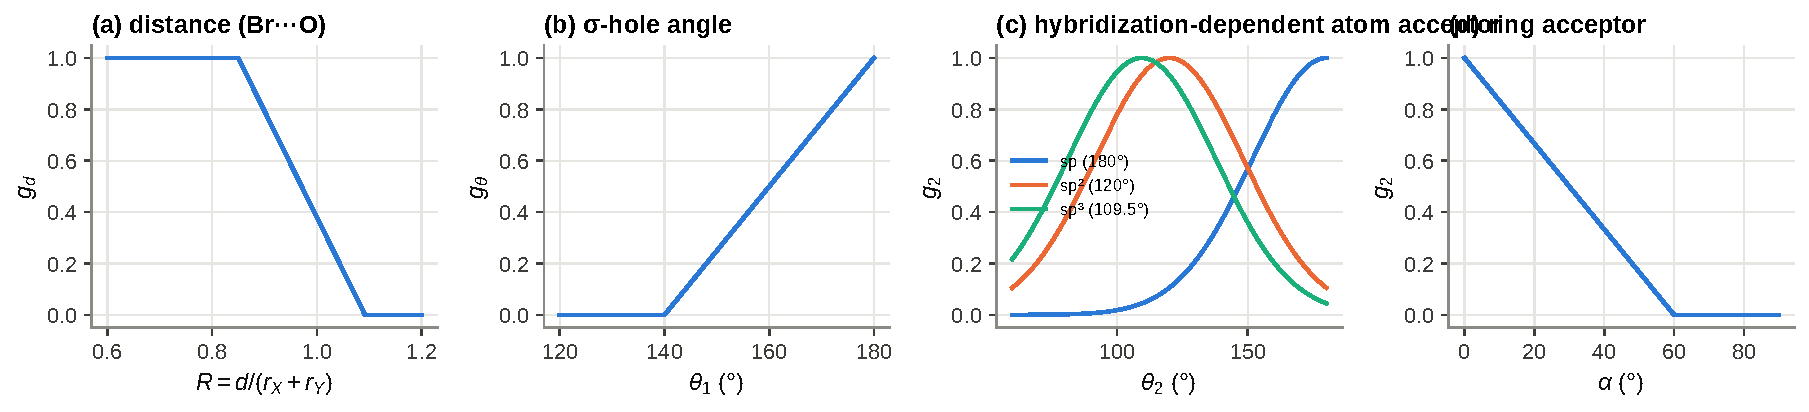
\includegraphics[width=0.82\textwidth]{FigS1_score_functions.pdf}
\caption{Terms of the geometric score with default parameters. (a) Distance term for Br$\cdots$O. (b) Angle term. (c) Acceptor term for lone pairs. (d) Acceptor term for rings.}
\label{fig:score}
\end{figure}

\paragraph{Tier T2.} $f=N_\mathrm{on}/N_\mathrm{frames}$, and $\tau$ is the mean length of unbroken runs multiplied by the saving interval $\Delta t$ (ps per analysed frame). The persistence score is
\begin{equation}
D=f\,\bigl[1-\exp(-\tau/\tau_0)\bigr]^{p},\qquad \tau_0 = \SI{100}{ps},\ p = 0.25,
\end{equation}
where the exponent applies to the residence factor only. Contacts below the reporting threshold (10\% by default) are hidden but kept.

\paragraph{Tier T3a.} The electron count is $N_e=\sum_i Z_i-q_1-q_2$. A link hydrogen sits on the cut bond at a fixed X--H length (C 1.09, N 1.01, O 0.96, and S \SI{1.34}{\angstrom}). MM residues farther than \SI{6}{\angstrom} from every halogen carry folded charges, $q_a^\mathrm{fold}=q_a+\sum_{h\in a}q_h$; closer residues carry explicit hydrogens built from the template with their own charges. The RC scheme\cite{LinTruhlar2005} sets the charge of M1 to zero and places $q_\mathrm{M1}/n_\mathrm{M2}$ at the midpoint of each M1--M2 bond; RCD adds $2q_\mathrm{M1}/n_\mathrm{M2}$ at each midpoint and subtracts $q_\mathrm{M1}/n_\mathrm{M2}$ from each M2, which preserves the M2--M1 bond dipoles. A residue cut by the boundary shifts its MM charges equally, so its total charge stays an integer. The MM charges alone give the potential $\phi_X=k\sum_i q_i/r_{iX}$ and the field $E_{AX}=k\sum_i q_i(\mathbf r_X-\mathbf r_i)\cdot\hat{\mathbf u}_{AX}/r_{iX}^3$ at the halogen ($k=\SI{14.3996}{V\,\angstrom\,e^{-1}}$).

\paragraph{Tiers T3b--T5.} The main text gives $\Sigma\ET$, the grey zone, $\chi_\mathrm{CT}$, and BXQI. The NPA charge transfer is $\Delta q_\mathrm{CT}=q_1^\mathrm{formal}-\sum_{i\in1}q_i^\mathrm{NPA}$, the charge moved from fragment~2 to fragment~1 (the halogen donor), and it is positive when fragment~1 gains electrons. Open-shell $\alpha$ and $\beta$ tables are added. As a check, the engine reproduces a hand-calculated example: $G=0.859$, $D(f = 0.62, \tau = \SI{160}{ps}) = 0.586$, and BXQI $=64.6$.

% ---- table from tables/tab_params.tex (generated) ----
{\scriptsize
\setlength{\tabcolsep}{3pt}
\begin{longtable}{llp{4.2cm}l}
\caption{Every adjustable parameter of \BX{} with its default value (99 parameters). All can be changed in the program, on each tier page, and on the \emph{All parameters} page.}\label{tab:params}\\
\toprule
Tier & Parameter & Meaning (unit) & Default\\
\midrule
\endfirsthead
\toprule
Tier & Parameter & Meaning (unit) & Default\\
\midrule
\endhead
\bottomrule
\endlastfoot
Structure & \texttt{struct.altloc} & Alternate locations & \parbox[t]{5.0cm}{\raggedright first listed (A / 1 / blank)}\\
Structure & \texttt{struct.bondTol} & Bond tolerance (\AA{}) & \parbox[t]{5.0cm}{\raggedright 0.45}\\
Geometry & \texttt{geom.cutoffs} & X$\cdots$Y distance cut-offs (\AA{}) & \parbox[t]{5.0cm}{\raggedright I: N 3.97, O 3.82, S 4.15, AR 4; BR: N 3.84, O 3.68, S 4.02, AR 3.87; CL: N 3.77, O 3.61, S 3.95, AR 3.8; F: N 3.32, O 3.29, S 3.57, AR 3.4}\\
Geometry & \texttt{geom.theta1Min} & $\theta_1$ minimum (A--X$\cdots$Y) ($^\circ$) & \parbox[t]{5.0cm}{\raggedright 140}\\
Geometry & \texttt{geom.theta1Max} & $\theta_1$ maximum ($^\circ$) & \parbox[t]{5.0cm}{\raggedright 180}\\
Geometry & \texttt{geom.theta2Use} & Filter on $\theta_2$ (X$\cdots$Y--R) & \parbox[t]{5.0cm}{\raggedright off}\\
Geometry & \texttt{geom.theta2Min} & $\theta_2$ minimum ($^\circ$) & \parbox[t]{5.0cm}{\raggedright 90}\\
Geometry & \texttt{geom.theta2Max} & $\theta_2$ maximum ($^\circ$) & \parbox[t]{5.0cm}{\raggedright 180}\\
Geometry & \texttt{geom.piNormalMax} & $\pi$ acceptor: max angle to ring normal ($^\circ$) & \parbox[t]{5.0cm}{\raggedright 60}\\
Geometry & \texttt{geom.includePi} & Aromatic $\pi$ acceptors (Phe/Tyr/Trp) & \parbox[t]{5.0cm}{\raggedright on}\\
Geometry & \texttt{geom.includeHisPi} & His ring as $\pi$ acceptor & \parbox[t]{5.0cm}{\raggedright off}\\
Geometry & \texttt{geom.includeNucleicPi} & Nucleobase rings as $\pi$ acceptors & \parbox[t]{5.0cm}{\raggedright on}\\
Geometry & \texttt{geom.includeLigandPi} & Ligand and cofactor rings as $\pi$ acceptors & \parbox[t]{5.0cm}{\raggedright off}\\
Geometry & \texttt{geom.acceptorScope.protein} & Protein N/O/S acceptors & \parbox[t]{5.0cm}{\raggedright on}\\
Geometry & \texttt{geom.acceptorScope.nucleic} & Nucleic-acid acceptors & \parbox[t]{5.0cm}{\raggedright on}\\
Geometry & \texttt{geom.acceptorScope.water} & Water O acceptors & \parbox[t]{5.0cm}{\raggedright off}\\
Geometry & \texttt{geom.acceptorScope.otherLigand} & Other ligands / cofactors as acceptors & \parbox[t]{5.0cm}{\raggedright off}\\
Geometry & \texttt{geom.excludeNonLewis} & Exclude poor Lewis bases & \parbox[t]{5.0cm}{\raggedright off}\\
Geometry & \texttt{geom.reportNearMiss} & Report near-misses & \parbox[t]{5.0cm}{\raggedright off}\\
Geometry & \texttt{geom.includeF} & Include C--F donors & \parbox[t]{5.0cm}{\raggedright off}\\
Geometry & \texttt{score.vdw} & van der Waals radii (Bondi) (\AA{}) & \parbox[t]{5.0cm}{\raggedright H 1.2, C 1.7, N 1.55, O 1.52, F 1.47, P 1.8, S 1.8, CL 1.75, BR 1.85, I 1.98, SE 1.9, B 1.92, SI 2.1}\\
Geometry & \texttt{score.ringRadius} & Ring pseudo-radius (\AA{}) & \parbox[t]{5.0cm}{\raggedright 1.77}\\
Geometry & \texttt{score.Rbest} & R for full distance score & \parbox[t]{5.0cm}{\raggedright 0.85}\\
Geometry & \texttt{score.Rflag} & Flag short contacts below R & \parbox[t]{5.0cm}{\raggedright 0.8}\\
Geometry & \texttt{score.Rshort} & Short-contact penalty starts at R & \parbox[t]{5.0cm}{\raggedright 0}\\
Geometry & \texttt{score.Rmin} & Short-contact penalty: g\_d = 0 at R & \parbox[t]{5.0cm}{\raggedright 0.6}\\
Geometry & \texttt{score.th2Opt} & Optimal $\theta_2$ for sp$^2$ acceptors ($^\circ$) & \parbox[t]{5.0cm}{\raggedright 120}\\
Geometry & \texttt{score.th2OptSP} & Optimal $\theta_2$ for sp acceptors ($^\circ$) & \parbox[t]{5.0cm}{\raggedright 180}\\
Geometry & \texttt{score.th2OptSP3} & Optimal $\theta_2$ for sp³ acceptors ($^\circ$) & \parbox[t]{5.0cm}{\raggedright 109.5}\\
Geometry & \texttt{score.th2Width} & $\theta_2$ width ($^\circ$) & \parbox[t]{5.0cm}{\raggedright 40}\\
Dynamics & \texttt{dyn.stride} & Frame stride & \parbox[t]{5.0cm}{\raggedright 1}\\
Dynamics & \texttt{dyn.occCut} & Occupancy cut-off (\%) & \parbox[t]{5.0cm}{\raggedright 10}\\
Dynamics & \texttt{dyn.dt} & Time between saved frames (ps) & \parbox[t]{5.0cm}{\raggedright 1}\\
Dynamics & \texttt{dyn.tauScale} & Residence scale $\tau_0$ (ps) & \parbox[t]{5.0cm}{\raggedright 100}\\
Dynamics & \texttt{dyn.dExp} & Residence exponent p & \parbox[t]{5.0cm}{\raggedright 0.25}\\
Geometry & \texttt{mat.images} & Periodic image shells (CIF) & \parbox[t]{5.0cm}{\raggedright 1}\\
Geometry & \texttt{mat.minDist} & Minimum X$\cdots$Y distance (CIF) (\AA{}) & \parbox[t]{5.0cm}{\raggedright 1.6}\\
QM model & \texttt{ff.name} & Force field (charges, protonation templates) & \parbox[t]{5.0cm}{\raggedright AMBER ff14SB + OL15/OL3}\\
QM model & \texttt{ff.water} & Water model & \parbox[t]{5.0cm}{\raggedright TIP3P}\\
QM model & \texttt{ff.hisDefault} & Histidine default & \parbox[t]{5.0cm}{\raggedright HIE / HSE (N$\varepsilon$--H, neutral)}\\
QM model & \texttt{ff.termini} & Chain termini & \parbox[t]{5.0cm}{\raggedright charged (NH$_3^+$ / COO$^-$)}\\
QM model & \texttt{ff.chainBreaks} & Chain breaks (missing residues) & \parbox[t]{5.0cm}{\raggedright treat as internal (no extra charge)}\\
QM model & \texttt{ff.ssCut} & Disulfide S--S cut-off (\AA{}) & \parbox[t]{5.0cm}{\raggedright 2.5}\\
QM model & \texttt{ff.chargeSource} & MM charge source & \parbox[t]{5.0cm}{\raggedright PQR charges from a loaded PQR file, otherwise force field}\\
QM model & \texttt{ff.foldH} & Missing hydrogens: fold charge onto parent atom & \parbox[t]{5.0cm}{\raggedright on}\\
QM model & \texttt{ff.missing} & Missing heavy atoms & \parbox[t]{5.0cm}{\raggedright spread their charge over the residue (keeps net charge)}\\
QM model & \texttt{qm.mode} & Acceptor residue in QM region & \parbox[t]{5.0cm}{\raggedright whole residue}\\
QM model & \texttt{qm.shell} & Extra QM shell around X (\AA{}) & \parbox[t]{5.0cm}{\raggedright 0}\\
QM model & \texttt{qm.keepAmide} & Keep the amide of backbone acceptors & \parbox[t]{5.0cm}{\raggedright backbone N acceptors: add the preceding residue (default)}\\
QM model & \texttt{qm.orientPolarH} & Orient added O--H and S--H hydrogens & \parbox[t]{5.0cm}{\raggedright on}\\
QM model & \texttt{qm.keepFileH} & Keep ligand hydrogens of the file & \parbox[t]{5.0cm}{\raggedright off}\\
QM model & \texttt{qm.shellWater} & Shell includes waters & \parbox[t]{5.0cm}{\raggedright off}\\
QM model & \texttt{qm.shellIons} & Shell includes ions & \parbox[t]{5.0cm}{\raggedright off}\\
QM model & \texttt{qm.forceH} & Re-protonate files with hydrogens & \parbox[t]{5.0cm}{\raggedright off}\\
QM model & \texttt{qm.linkScheme} & Link-atom position & \parbox[t]{5.0cm}{\raggedright fixed X--H bond length along the cut bond}\\
QM model & \texttt{qm.xh} & X--H bond lengths (\AA{}) & \parbox[t]{5.0cm}{\raggedright C 1.09, N 1.01, O 0.96, S 1.34, P 1.42, B 1.19, SE 1.46}\\
QM model & \texttt{qm.ligandCharge} & Ligand net charge & \parbox[t]{5.0cm}{\raggedright MOL2 total from a loaded file, otherwise the ligand structure with pH-7 rules}\\
QM model & \texttt{qm.polarHRotamer} & H rotamer near halogens & \parbox[t]{5.0cm}{\raggedright best hydrogen bond, all acceptors alike (default)}\\
QM model & \texttt{qm.hbShell} & Add N--H/O--H donors near X (\AA{}) & \parbox[t]{5.0cm}{\raggedright 3.6}\\
QM model & \texttt{qm.basicAmines} & Aliphatic amines of ligands & \parbox[t]{5.0cm}{\raggedright keep neutral and warn (default)}\\
QM model & \texttt{qm.env} & Environment & \parbox[t]{5.0cm}{\raggedright QM cluster (optionally in a dielectric)}\\
QM model & \texttt{qm.pcm} & Cluster: implicit dielectric & \parbox[t]{5.0cm}{\raggedright on}\\
QM model & \texttt{qm.eps} & Dielectric constant $\varepsilon$ & \parbox[t]{5.0cm}{\raggedright 4}\\
QM model & \texttt{qm.program} & QM program (NBO job) & \parbox[t]{5.0cm}{\raggedright Gaussian 16 (tested)}\\
QM model & \texttt{qm.allowUntested} & Allow untested routes & \parbox[t]{5.0cm}{\raggedright off}\\
QM model & \texttt{qm.method} & Method & \parbox[t]{5.0cm}{\raggedright wB97XD}\\
QM model & \texttt{qm.basis} & Basis set & \parbox[t]{5.0cm}{\raggedright def2TZVP}\\
QM model & \texttt{qm.nproc} & Cores & \parbox[t]{5.0cm}{\raggedright 16}\\
QM model & \texttt{qm.mem} & Memory & \parbox[t]{5.0cm}{\raggedright 32GB}\\
QM model & \texttt{qm.nbo7} & Gaussian: pop=nbo7 (licensed NBO 7; untested) & \parbox[t]{5.0cm}{\raggedright off}\\
QM model & \texttt{mm.radius} & Embedding radius (\AA{}) & \parbox[t]{5.0cm}{\raggedright 0}\\
QM model & \texttt{mm.selection} & Embedding selection & \parbox[t]{5.0cm}{\raggedright whole residues (keeps residue charges integral)}\\
QM model & \texttt{mm.boundary} & QM/MM boundary charges & \parbox[t]{5.0cm}{\raggedright RC: move q(M1) to M1--M2 bond midpoints (Lin \& Truhlar)}\\
QM model & \texttt{mm.explicitH} & Explicit MM hydrogens within (\AA{}) & \parbox[t]{5.0cm}{\raggedright 6}\\
QM model & \texttt{mm.neutralizeCut} & Integer charge for cut residues & \parbox[t]{5.0cm}{\raggedright on}\\
NBO screen & \texttt{nbo.threshold} & Nominal threshold $\Sigma$E(2) (kcal/mol) & \parbox[t]{5.0cm}{\raggedright 0.5}\\
NBO screen & \texttt{nbo.hbFlagMin} & Competing H-bond flag: minimum X$\to\sigma$*(N--H/O--H) (kcal/mol) & \parbox[t]{5.0cm}{\raggedright 0.5}\\
NBO screen & \texttt{nbo.greyLow} & Grey zone: lower limit (kcal/mol) & \parbox[t]{5.0cm}{\raggedright 0.3}\\
NBO screen & \texttt{nbo.greyHigh} & Grey zone: upper limit (kcal/mol) & \parbox[t]{5.0cm}{\raggedright 0.8}\\
NBO screen & \texttt{nbo.includeRY} & Count n$\to$RY*(X) terms in the decision & \parbox[t]{5.0cm}{\raggedright off}\\
NBO screen & \texttt{nbo.geomTol} & Geometry check tolerance (\AA{}) & \parbox[t]{5.0cm}{\raggedright 0.05}\\
ALMO-EDA & \texttt{eda.method} & EDA method & \parbox[t]{5.0cm}{\raggedright wB97X-V}\\
ALMO-EDA & \texttt{eda.basis} & EDA basis & \parbox[t]{5.0cm}{\raggedright def2-TZVPD}\\
ALMO-EDA & \texttt{eda.preset} & EDA2 preset & \parbox[t]{5.0cm}{\raggedright 1 $\cdot$ frozen decomposition + nMDQ-uFERF POL (standard)}\\
ALMO-EDA & \texttt{eda.bsse} & EDA\_BSSE (counterpoise for CT) & \parbox[t]{5.0cm}{\raggedright on}\\
ALMO-EDA & \texttt{eda.covp} & COVP analysis & \parbox[t]{5.0cm}{\raggedright off}\\
ALMO-EDA & \texttt{eda.pcm} & PCM solvent & \parbox[t]{5.0cm}{\raggedright off}\\
ALMO-EDA & \texttt{eda.eps} & PCM $\varepsilon$ & \parbox[t]{5.0cm}{\raggedright 4}\\
ALMO-EDA & \texttt{eda.memMB} & MEM\_TOTAL (MB) & \parbox[t]{5.0cm}{\raggedright 32000}\\
ALMO-EDA & \texttt{eda.chiHigh} & $\chi$\_CT for CT-driven & \parbox[t]{5.0cm}{\raggedright 0.6}\\
ALMO-EDA & \texttt{eda.chiLow} & $\chi$\_CT for polarization-driven & \parbox[t]{5.0cm}{\raggedright 0.4}\\
BXQI & \texttt{bxqi.weights} & Tier weights & \parbox[t]{5.0cm}{\raggedright G 0.25, D 0.2, E 0.3, C 0.25}\\
BXQI & \texttt{bxqi.E0} & E$_0$ (NBO saturation) (kcal/mol) & \parbox[t]{5.0cm}{\raggedright 2}\\
BXQI & \texttt{bxqi.C0} & C$_0$ (EDA saturation) (kcal/mol) & \parbox[t]{5.0cm}{\raggedright 2.4}\\
BXQI & \texttt{bxqi.useC} & Use the EDA total in the index & \parbox[t]{5.0cm}{\raggedright on}\\
BXQI & \texttt{bxqi.consE2hi} & Consistency: large E(2) (kcal/mol) & \parbox[t]{5.0cm}{\raggedright 1}\\
BXQI & \texttt{bxqi.consCTlo} & Consistency: negligible CT (kcal/mol) & \parbox[t]{5.0cm}{\raggedright 0.1}\\
BXQI & \texttt{bxqi.consE2lo} & Consistency: small E(2) (kcal/mol) & \parbox[t]{5.0cm}{\raggedright 0.25}\\
BXQI & \texttt{bxqi.consCThi} & Consistency: large CT (kcal/mol) & \parbox[t]{5.0cm}{\raggedright 1}\\
\end{longtable}}
% ---- end of tables/tab_params.tex ----

%% =====================================================================
\section{Force-Field Data and Ligand Charges}
\label{sec:ff}

The script \texttt{tools/extract\_ff.py} reads the OpenMM force-field files.\cite{Eastman2017} The tables hold 110 residue variants for ff14SB and ff19SB\cite{Maier2015,Tian2020} and 105 variants for CHARMM36,\cite{Best2012} each with an integer net charge. Table~\ref{tab:ffref} compares the charges with the PDB2PQR reference files.\cite{Jurrus2018} Because the AMBER rows share the parameter source with PDB2PQR, they test the template matching, the termini, and the protonation handling, and the hydrogen columns show that folding does not hide errors in the hydrogen charges.

% ---- table from tables/tab_ffref.tex (generated) ----
\begin{table}[!htbp]\centering\scriptsize\setlength{\tabcolsep}{3pt}
\caption{Force-field charges of \BX{} compared with the PDB2PQR reference files.\cite{Jurrus2018} Heavy atoms: charge of each heavy atom plus its hydrogens on both sides. Hydrogens: every hydrogen of the reference file against the template charge of the same hydrogen name, without folding. Both programs read the same AMBER parameter files, so the AMBER rows test the template matching, termini, and protonation handling of \BX{}, not the charges themselves. PDB2PQR ships CHARMM22 charges; the CHARMM36 rows only show that \BX{} differs from CHARMM22 where CHARMM36 changed the parameters (tryptophan).}\label{tab:ffref}
\resizebox{\textwidth}{!}{\begin{tabular}{llrrrrrl}\toprule PDB & Force field (BondX vs.\ reference) & Residues & Heavy atoms & max $|\Delta q|$ (e) & Hydrogens & max $|\Delta q_\mathrm{H}|$ (e) & Differences\\\midrule
1AFS & ff14SB vs.\ AMBER (PDB2PQR) & 663 & 5140 & 0 & 5168 & 0 & \\
1AJJ & ff14SB vs.\ AMBER (PDB2PQR) & 36 & 274 & 0 & 228 & 0 & \\
1BX8 & ff14SB vs.\ AMBER (PDB2PQR) & 46 & 334 & 0 & 314 & 0 & \\
1A1P & ff14SB vs.\ AMBER (PDB2PQR) & 13 & 107 & 0 & 97 & 0 & \\
1AFS & CHARMM36 vs.\ CHARMM22 (PDB2PQR) & 663 & 5102 & 0.13 & 5168 & 0.1 & Trp only (C36 update)\\
1AJJ & CHARMM36 vs.\ CHARMM22 (PDB2PQR) & 30 & 237 & 0.13 & 204 & 0.1 & Trp only (C36 update)\\
1BX8 & CHARMM36 vs.\ CHARMM22 (PDB2PQR) & 35 & 266 & 0 & 270 & 0 & \\
\bottomrule\end{tabular}}\end{table}
% ---- end of tables/tab_ffref.tex ----

Without a MOL2 file, \BX{} builds one Kekul\'e structure for the ligand. Every sp$^2$ carbon receives one double bond, the structure with the most C=O bonds wins, an sp$^2$ N without a double bond carries one H, and a pyridinium-type N with three neighbours carries $+1$. At pH~7, carboxylic, phosphoric, phosphonic, sulfonic, and sulfuric acids lose their O--H hydrogen. Aliphatic amines, tetrazoles, and acyl sulfonamides are flagged with a warning; basic amines can be protonated with one switch (\texttt{qm.basicAmines}). The PDB formula (FORMUL record) checks the result, and each covalent link to another residue removes one H from the expected count. The rules give $-1$ for IDD594 (1US0), $-2$ for brivudine monophosphate (2W0S), and $-3$ for the 4GQL inhibitor, and TBS (1P5E) is neutral with one N--H.

%% =====================================================================
\section{Geometric Tier}
\label{sec:t1}

% Original HAL59 scope paragraph retained for reference.
% Figure~\ref{fig:scans} gives $G$ along the rigid scans, in which the acceptor moves as a rigid body. Table~\ref{tab:hal59} lists the T1 results of all 59 HAL59 dimers, and Table~\ref{tab:protT1} lists the 15 contacts of the protein test set at default settings: nine distinct contacts, five replicas in other chains, and the 4DST contact repeated in its polar-hydrogen copy.
\tcb{The full HAL59 table retains all 59 dimers for transparency, including exploratory electronic-structure cases. T1 performance is evaluated only for the 29 dimers with C-bound Cl, Br, or I donors. Of these, 23 also have acceptors within the implemented T1 scope (protein/nucleic-acid N and O, protein S, or aromatic rings); six P- or F-acceptor dimers have no default T1 cut-off. The 27 non-C-bound-donor dimers, including FI$\cdots$pyridine ($\Sigma E^{(2)}=72.2$~kcal~mol$^{-1}$), are not counted in T1 sensitivity or correlation statistics. Figure~\ref{fig:scans} gives $G$ along the rigid scans, in which the acceptor moves as a rigid body. Table~\ref{tab:hal59} lists the T1 results of all 59 HAL59 dimers, and Table~\ref{tab:protT1} lists the 15 contacts of the protein test set at default settings: nine distinct contacts, five replicas in other chains, and the 4DST contact repeated in its polar-hydrogen copy.}

\begin{figure}[!htbp]
\centering
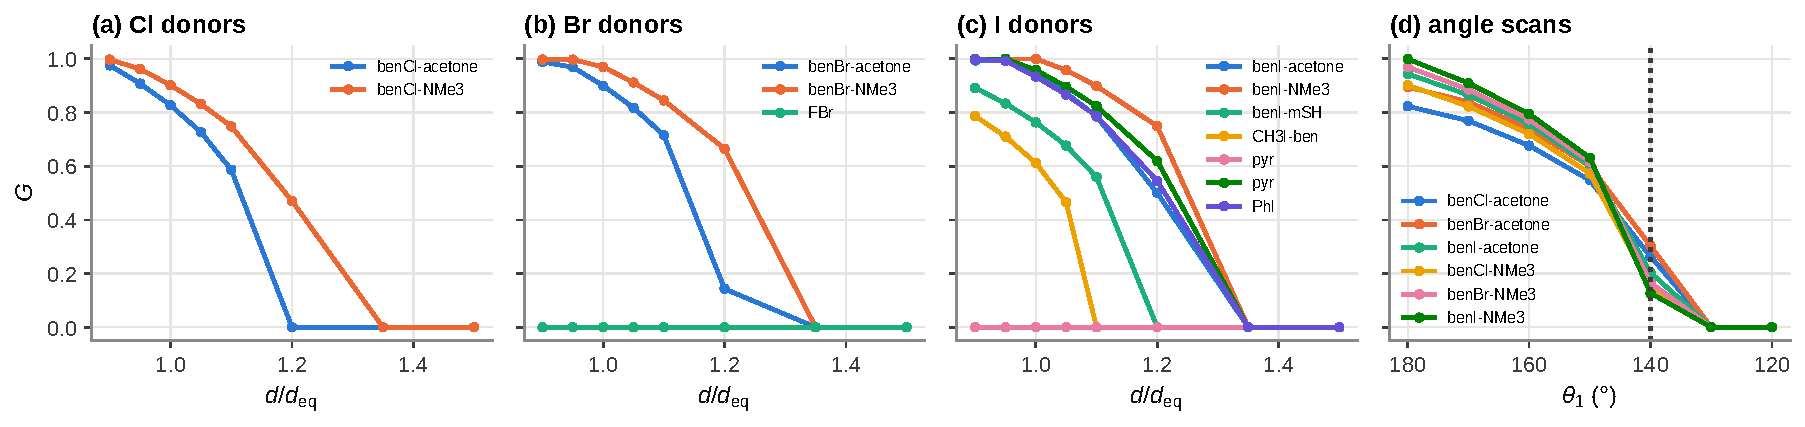
\includegraphics[width=0.85\textwidth]{FigS2_scans_T1.pdf}
\caption{Geometric score $G$ along the rigid scans. (a--c) Distance scans by donor halogen. (d) Angle scans. Dotted line: $\theta_1=140^\circ$.}
\label{fig:scans}
\end{figure}

% ---- table from tables/tab_hal59_t1.tex (generated) ----
{\scriptsize
\setlength{\tabcolsep}{3pt}
\begin{longtable}{llllrrrrllrl}
\caption{HAL59 dimers. Reference binding energies: CCSD(T)/CBS (kcal\,mol$^{-1}$, GMTKN55). Tier T1 of \BX{} on the reference geometries. Covered: a default cut-off exists for the X/Y pair.}\label{tab:hal59}\\
\toprule
Dimer & Set & X & Y & $E_\mathrm{ref}$ & $d$ (\AA) & $\theta_1$ & $\theta_2$ & Covered & T1 & $G$ & Role\\
\midrule
\endfirsthead
\toprule
Dimer & Set & X & Y & $E_\mathrm{ref}$ & $d$ (\AA) & $\theta_1$ & $\theta_2$ & Covered & T1 & $G$ & Role\\
\midrule
\endhead
\bottomrule
\endlastfoot
PCH\_PhBr & XB51 & Br & P & 0.85 & 3.634 & 180.0 & 180 & no & no & 0.000 & \\
NCH\_PhBr & XB51 & Br & N & 1.15 & 3.189 & 180.0 & 180 & yes & yes & 0.881 & \\
NH3\_PhBr & XB51 & Br & N & 2.02 & 3.138 & 179.9 & 111 & yes & yes & 0.903 & \\
MeI\_PCH & XB51 & I & P & 0.85 & 3.771 & 180.0 & 180 & no & no & 0.000 & \\
MeI\_NCH & XB51 & I & N & 1.42 & 3.288 & 180.0 & 180 & yes & yes & 0.889 & \\
MeI\_NH3 & XB51 & I & N & 2.73 & 3.210 & 180.0 & 111 & yes & yes & 0.922 & \\
PCH\_PhI & XB51 & I & P & 0.92 & 3.764 & 180.0 & 180 & no & no & 0.000 & \\
NCH\_PhI & XB51 & I & N & 1.87 & 3.259 & 180.0 & 180 & yes & yes & 0.902 & \\
NH3\_PhI & XB51 & I & N & 3.33 & 3.177 & 179.8 & 111 & yes & yes & 0.933 & \\
PCH\_F3CI & XB51 & I & P & 0.89 & 3.724 & 180.0 & 180 & no & no & 0.000 & \\
NCH\_F3CI & XB51 & I & N & 3.61 & 3.105 & 180.0 & 180 & yes & yes & 0.963 & \\
NH3\_F3CI & XB51 & I & N & 5.88 & 2.992 & 180.0 & 111 & yes & yes & 1.000 & \\
BrBr\_PCH & XB51 & Br & P & 1.18 & 3.443 & 180.0 & 180 & no & no & 0.000 & \\
BrBr\_NCH & XB51 & Br & N & 3.61 & 2.868 & 180.0 & 180 & no & no & 0.000 & \\
BrBr\_NH3 & XB51 & Br & N & 7.29 & 2.670 & 180.0 & 111 & no & no & 0.000 & \\
PCH\_NBS & XB51 & Br & P & 1.19 & 3.410 & 180.0 & 180 & no & no & 0.000 & \\
NCH\_NBS & XB51 & Br & N & 4.32 & 2.816 & 180.0 & 180 & no & no & 0.000 & \\
NH3\_NBS & XB51 & Br & N & 8.02 & 2.663 & 180.0 & 111 & no & no & 0.000 & \\
PCH\_FCl & XB51 & Cl & P & 1.16 & 3.163 & 180.0 & 180 & no & no & 0.000 & \\
NCH\_FCl & XB51 & Cl & N & 4.81 & 2.613 & 180.0 & 180 & no & no & 0.000 & \\
NH3\_FCl & XB51 & Cl & N & 10.54 & 2.348 & 180.0 & 110 & no & no & 0.000 & \\
PCH\_NIS & XB51 & I & P & 1.53 & 3.496 & 180.0 & 180 & no & no & 0.000 & \\
NCH\_NIS & XB51 & I & N & 5.91 & 2.862 & 180.0 & 180 & no & no & 0.000 & \\
NH3\_NIS & XB51 & I & N & 10.99 & 2.694 & 179.9 & 111 & no & no & 0.000 & \\
PCH\_FBr & XB51 & Br & P & 2.07 & 3.088 & 180.0 & 180 & no & no & 0.000 & \\
NCH\_FBr & XB51 & Br & N & 7.53 & 2.529 & 180.0 & 180 & no & no & 0.000 & \\
NH3\_FBr & XB51 & Br & N & 15.30 & 2.357 & 180.0 & 110 & no & no & 0.000 & \\
FI\_PCH & XB51 & I & P & 2.74 & 3.178 & 180.0 & 180 & no & no & 0.000 & \\
FI\_NCH & XB51 & I & N & 9.33 & 2.615 & 180.0 & 180 & no & no & 0.000 & \\
FI\_NH3 & XB51 & I & N & 17.11 & 2.509 & 180.0 & 111 & no & no & 0.000 & \\
MeI\_FCCH & XB51 & I & F & 0.50 & 3.399 & 180.0 & 180 & no & no & 0.000 & \\
BrBr\_FCCH & XB51 & Br & F & 0.74 & 3.191 & 180.0 & 180 & no & no & 0.000 & \\
FI\_FCCH & XB51 & I & F & 0.29 & 4.947 & 0.0 & 180 & no & no & 0.000 & control\\
MeI\_FMe & XB51 & I & F & 1.70 & 3.188 & 171.5 & 105 & no & no & 0.000 & \\
BrBr\_FMe & XB51 & Br & F & 2.87 & 2.811 & 173.9 & 111 & no & no & 0.000 & \\
FI\_FMe & XB51 & I & F & 5.97 & 2.664 & 179.0 & 120 & no & no & 0.000 & \\
MeI\_OCH2 & XB51 & I & O & 2.39 & 3.176 & 170.5 & 103 & yes & yes & 0.809 & \\
BrBr\_OCH2 & XB51 & Br & O & 4.41 & 2.757 & 173.7 & 110 & no & no & 0.000 & \\
FI\_OCH2 & XB51 & I & O & 9.94 & 2.577 & 178.8 & 120 & no & no & 0.000 & \\
MeI\_OPH3 & XB51 & I & O & 3.34 & 3.145 & 169.8 & 98 & yes & yes & 0.804 & \\
BrBr\_OPH3 & XB51 & Br & O & 5.95 & 2.682 & 176.1 & 110 & no & no & 0.000 & \\
FI\_OPH3 & XB51 & I & O & 13.36 & 2.503 & 178.3 & 116 & no & no & 0.000 & \\
MeI\_pyr & XB51 & I & N & 3.61 & 3.116 & 180.0 & 121 & yes & yes & 0.958 & \\
BrBr\_pyr & XB51 & Br & N & 9.07 & 2.578 & 180.0 & 121 & no & no & 0.000 & \\
FI\_pyr & XB51 & I & N & 20.34 & 2.428 & 180.0 & 120 & no & no & 0.000 & \\
11\_benF3-ben & X40 & F & ring & 4.40 & 4.078 & 62.0 & -- & yes & no & 0.000 & control\\
12\_benF6-ben & X40 & F & ring & 6.12 & 3.734 & 63.5 & -- & yes & no & 0.000 & control\\
19\_benCl-acetone & X40 & Cl & O & 1.49 & 3.124 & 178.8 & 117 & yes & yes & 0.827 & \\
20\_benBr-acetone & X40 & Br & O & 2.43 & 3.065 & 178.6 & 120 & yes & yes & 0.900 & \\
21\_benI-acetone & X40 & I & O & 3.46 & 3.094 & 179.6 & 125 & yes & yes & 0.945 & \\
22\_benCl-Nm3 & X40 & Cl & N & 2.11 & 3.057 & 179.7 & 108 & yes & yes & 0.901 & \\
23\_benBr-Nm3 & X40 & Br & N & 3.78 & 2.965 & 179.7 & 108 & yes & yes & 0.970 & \\
24\_benI-Nm3 & X40 & I & N & 5.81 & 2.968 & 179.9 & 108 & yes & yes & 0.999 & \\
25\_benBr-mSH & X40 & Br & S & 2.32 & 3.542 & 167.0 & 85 & yes & yes & 0.668 & \\
26\_benI-mSH & X40 & I & S & 3.08 & 3.562 & 170.8 & 93 & yes & yes & 0.763 & \\
27\_CH3Br-ben & X40 & Br & ring & 1.81 & 3.554 & 164.2 & -- & yes & yes & 0.602 & \\
28\_CH3I-ben & X40 & I & ring & 2.48 & 3.673 & 165.2 & -- & yes & yes & 0.612 & \\
29\_CF3Br-ben & X40 & Br & ring & 3.11 & 3.407 & 164.0 & -- & yes & yes & 0.686 & \\
30\_CF3I-ben & X40 & I & ring & 3.91 & 3.534 & 163.3 & -- & yes & yes & 0.670 & \\
\end{longtable}}
% ---- end of tables/tab_hal59_t1.tex ----
% ---- table from tables/tab_protein_t1.tex (generated) ----
{\scriptsize
\setlength{\tabcolsep}{3pt}
\begin{longtable}{lllllp{1.9cm}rrrlr}
\caption{Halogen bonds found by tier T1 with default settings in the protein test set (all chains).}\label{tab:protT1}\\
\toprule
PDB & Donor & X & Acceptor & Y & Class & $d$ (\AA) & $\theta_1$ & $\theta_2$/$\alpha$ & Lewis & $G$\\
\midrule
\endfirsthead
\toprule
PDB & Donor & X & Acceptor & Y & Class & $d$ (\AA) & $\theta_1$ & $\theta_2$/$\alpha$ & Lewis & $G$\\
\midrule
\endhead
\bottomrule
\endlastfoot
1P5E & TBS302:C & BR11 & LEU83:C & O & backbone C=O & 2.876 & 176.9 & 121.2 & strong & 0.969\\
1P5E & TBS301:A & BR11 & LEU83:A & O & backbone C=O & 2.904 & 164.7 & 132.0 & strong & 0.826\\
1P5E & TBS302:C & BR12 & GLU81:C & O & backbone C=O & 3.048 & 171.7 & 151.5 & strong & 0.779\\
1P5E & TBS301:A & BR12 & GLU81:A & O & backbone C=O & 3.007 & 168.5 & 154.9 & strong & 0.756\\
1P5E & TBS302:C & BR13 & PHE80:C & $\pi$(ring) & aromatic $\pi$ & 3.680 & 174.8 & 30.4 & strong & 0.538\\
1P5E & TBS301:A & BR13 & PHE80:A & $\pi$(ring) & aromatic $\pi$ & 3.491 & 153.8 & 22.6 & strong & 0.511\\
1P5E & TBS301:A & BR10 & ILE10:A & O & backbone C=O & 3.238 & 144.1 & 110.1 & strong & 0.377\\
1US0+IDD594 & LDT320:A & BR8 & THR113:A & OG1 & hydroxyl O & 2.973 & 152.8 & 132.3 & strong & 0.641\\
2W0S & BVP1207:A & BR & ASN65:A & OD1 & amide C=O & 2.687 & 168.3 & 134.5 & strong & 0.872\\
2W0S & BVP1207:B & BR & ASN65:B & OD1 & amide C=O & 2.824 & 155.9 & 132.8 & strong & 0.724\\
4AGL & P84400:B & I15 & LEU145:B & O & backbone C=O & 2.980 & 172.0 & 119.5 & strong & 0.926\\
4AGL & P84400:A & I15 & LEU145:A & O & backbone C=O & 3.010 & 171.6 & 118.7 & strong & 0.911\\
4DST & 9LI201:A & CL2 & GLY75:A & N & backbone N--H & 3.520 & 140.5 & 73.1 & weak & 0.124\\
4DST (polar H) & 9LI201:A & CL2 & GLY75:A & N & backbone N--H & 3.520 & 140.5 & 73.1 & weak & 0.124\\
4GQL & R47306:A & CL1 & PRO232:A & O & backbone C=O & 2.688 & 166.7 & 119.4 & strong & 0.874\\
\end{longtable}}
% ---- end of tables/tab_protein_t1.tex ----

%% =====================================================================
\section{Protein QM Models and the MM Field}
\label{sec:models}

Table~\ref{tab:models} lists all 89 models. Figure~\ref{fig:size} shows the QM size against the shell radius and the MM potential at the halogen against the embedding radius. The FORMUL check confirms the ligand hydrogens of 1P5E, 2W0S, 4DST, and 4GQL. The 4GQL file lacks two polar ligand hydrogens, which \BX{} rebuilt. The 4AGL ligand P84 has 13 of its 21 heavy atoms; the model contains the resolved part with its open valences filled by hydrogens, and its charge is zero. Over the whole test set, the hydrogen count matches the formula for 191 of 214 complete ligand residues without metal, and the mismatches are listed in \texttt{results/ligand\_check.csv}. Sulfate ions in 2W0S carry $-2$, phosphothreonine in 1P5E carries $-2$, and neutral additives (glycerol, ethylene glycol, and DMSO) carry zero charge.

% Original edition-comparison wording removed; saved model settings retained.
% The 89 protein models were built with \BX{} 2.0, which differs from the defaults of version 3.0 in four settings. (1) A backbone N acceptor whose preceding residue was not in the model received a link hydrogen in place of the carbonyl carbon, which makes the Gly75 N of 4DST an amine; version 3.0 adds the preceding residue. (2) Added hydroxyl hydrogens kept their template rotamer, so that the Thr113 OG1 hydrogen of 1US0 points at the bromine (H$\cdots$Br \SI{2.20}{\angstrom}); version 3.0 scores N, O, and halogen acceptors alike, which turns this hydrogen to an oxygen acceptor (H$\cdots$Br \SI{3.48}{\angstrom}), and the forced halogen-directed rotamer gives H$\cdots$Br \SI{2.61}{\angstrom}. The deposited 1US0 entry contains no hydrogen coordinates for Thr113. (3) MM hydrogen charges were folded onto their heavy atoms everywhere; version 3.0 keeps explicit hydrogens within \SI{6}{\angstrom} of the halogen (Table~\ref{tab:field}). (4) The embedding radius was \SI{15}{\angstrom}; version 3.0 embeds the whole structure. In addition, version 3.0 adds every residue with an N--H or O--H group within \SI{3.6}{\angstrom} of the halogen to fragment~2; for the six systems, this adds Lys105 and Tyr144 (2W0S chain A), Lys105 (chain B), two water molecules (1P5E chain A), one water molecule (1P5E chain C and 4GQL), and nothing for 1US0, 4AGL, and 4DST. Lys105 is the donor of the N--H$\cdots$Br hydrogen bond seen in the larger 2W0S shells. Sets G and J (Section~\ref{sec:hardneg}) were built with all defaults of version 3.0; no QM/MM model with explicit MM hydrogens and whole-structure embedding was computed.
\tcb{The 89 saved set-F protein models used four documented model choices: (1) backbone-N sites at model boundaries were capped with link hydrogens when the preceding carbonyl residue was not included, so the 4DST Gly75 N was represented as an amine; (2) added hydroxyl hydrogens retained their template rotamers, including the 1US0 Thr113 O--H orientation toward Br (H$\cdots$Br = 2.20~\AA{}); (3) MM hydrogen charges were folded onto parent heavy atoms throughout the MM region; and (4) the embedding radius was 15~\AA{}. The saved set-G and set-J models include the explicit choices recorded in their manifests; set J contains the intact Gly75 amide. Model differences are described as saved input choices, not as separate BondX Studio versions.}

\begin{figure}[!htbp]
\centering
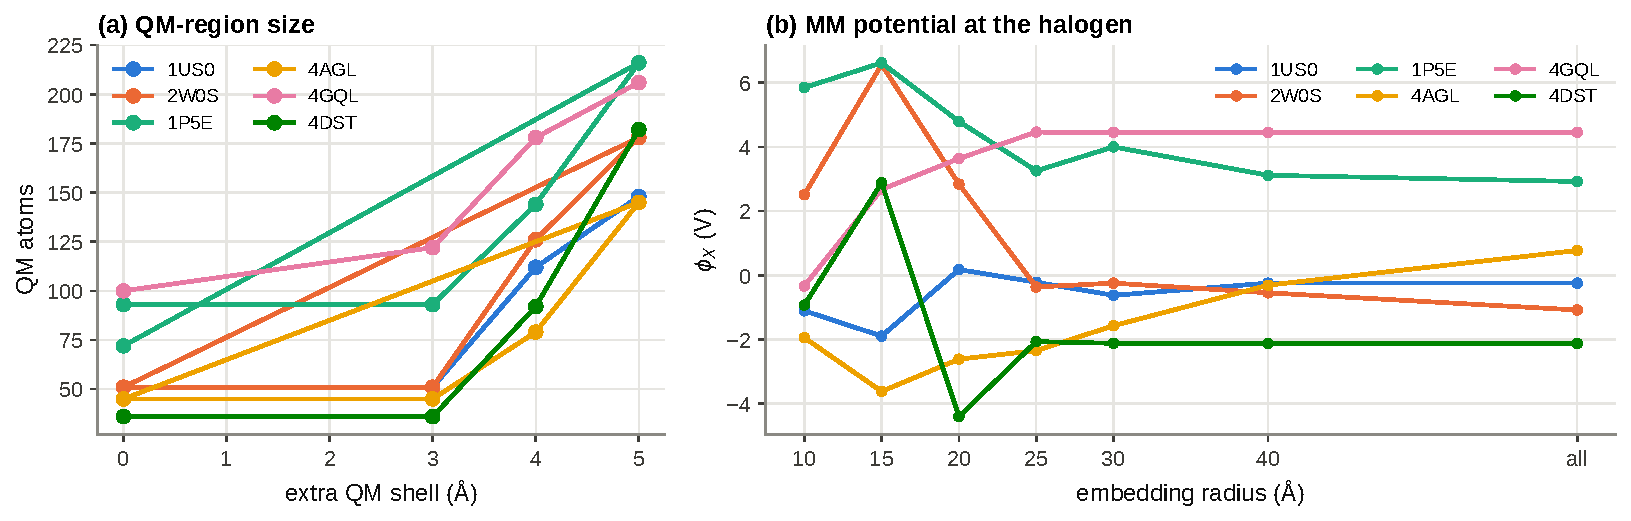
\includegraphics[width=0.9\textwidth]{FigS3_size_potential.pdf}
\caption{(a) QM cluster size against the extra shell radius. (b) MM potential at the halogen against the embedding radius (ff14SB, RC, explicit hydrogens within \SI{6}{\angstrom}); ``all'': whole structure.}
\label{fig:size}
\end{figure}

% ---- table from tables/tab_protein_models.tex (generated) ----
{\scriptsize
\setlength{\tabcolsep}{3pt}
\begin{longtable}{lllrrrlrrrrr}
\caption{All 89 protein QM models built by \BX{}. Atoms: QM atoms. +H: added hydrogens. Link: link hydrogens. $q_1/q_2$: fragment charges. $N_e$: electrons. MM $n$ and MM $Q$: number and net charge of the MM point charges. $\phi_X$ and $E_{AX}$: MM potential and field component at the halogen.}\label{tab:models}\\
\toprule
System & Ligand & Variant & Atoms & +H & Link & $q_1/q_2$ & $N_e$ & MM $n$ & MM $Q$ & $\phi_X$ (V) & $E_{AX}$ (V/\AA)\\
\midrule
\endfirsthead
\toprule
System & Ligand & Variant & Atoms & +H & Link & $q_1/q_2$ & $N_e$ & MM $n$ & MM $Q$ & $\phi_X$ (V) & $E_{AX}$ (V/\AA)\\
\midrule
\endhead
\bottomrule
\endlastfoot
1US0 & LDT:A:320 & cluster pcm4 & 51 & 7 & 2 & -1/0 & 264 & -- & -- & -- & --\\
1US0 & LDT:A:320 & cluster gas & 51 & 7 & 2 & -1/0 & 264 & -- & -- & -- & --\\
1US0 & LDT:A:320 & qmmm ff14SB & 51 & 7 & 2 & -1/0 & 264 & 1230 & -3.000 & -2.19 & 0.222\\
1US0 & LDT:A:320 & qmmm charmm36 & 51 & 7 & 2 & -1/0 & 264 & 898 & -3.000 & -2.16 & 0.210\\
1US0 & LDT:A:320 & qmmm Z1 & 51 & 7 & 2 & -1/0 & 264 & 1227 & -3.446 & -3.17 & 0.333\\
1US0 & LDT:A:320 & qmmm Z2 & 51 & 7 & 2 & -1/0 & 264 & 1224 & -3.023 & -2.35 & 0.239\\
1US0 & LDT:A:320 & qmmm Z3 & 51 & 7 & 2 & -1/0 & 264 & 1221 & -3.409 & -2.91 & 0.301\\
1US0 & LDT:A:320 & qmmm r10 & 51 & 7 & 2 & -1/0 & 264 & 683 & -2.000 & -1.41 & 0.205\\
1US0 & LDT:A:320 & qmmm r20 & 51 & 7 & 2 & -1/0 & 264 & 1887 & 1.000 & -0.12 & 0.235\\
1US0 & LDT:A:320 & qmmm r25 & 51 & 7 & 2 & -1/0 & 264 & 2328 & 0.000 & -0.52 & 0.236\\
1US0 & LDT:A:320 & qmmm full & 51 & 7 & 2 & -1/0 & 264 & 2485 & 0.000 & -0.54 & 0.234\\
1US0 & LDT:A:320 & shell3 & 51 & 7 & 2 & -1/0 & 264 & -- & -- & -- & --\\
1US0 & LDT:A:320 & shell4 & 112 & 31 & 8 & -1/0 & 500 & -- & -- & -- & --\\
1US0 & LDT:A:320 & shell5 & 148 & 45 & 12 & -1/0 & 644 & -- & -- & -- & --\\
2W0S & BVP:A:1207 & cluster pcm4 & 51 & 18 & 2 & -2/0 & 270 & -- & -- & -- & --\\
2W0S & BVP:A:1207 & cluster gas & 51 & 18 & 2 & -2/0 & 270 & -- & -- & -- & --\\
2W0S & BVP:A:1207 & qmmm ff14SB & 51 & 18 & 2 & -2/0 & 270 & 1163 & 5.000 & 6.28 & -0.195\\
2W0S & BVP:A:1207 & qmmm charmm36 & 51 & 18 & 2 & -2/0 & 270 & 830 & 5.000 & 6.32 & -0.279\\
2W0S & BVP:A:1207 & qmmm Z1 & 51 & 18 & 2 & -2/0 & 270 & 1160 & 4.546 & 4.73 & -0.115\\
2W0S & BVP:A:1207 & qmmm Z2 & 51 & 18 & 2 & -2/0 & 270 & 1157 & 5.065 & 6.39 & -0.142\\
2W0S & BVP:A:1207 & qmmm Z3 & 51 & 18 & 2 & -2/0 & 270 & 1153 & 4.361 & 4.86 & -0.110\\
2W0S & BVP:A:1207 & qmmm r10 & 51 & 18 & 2 & -2/0 & 270 & 652 & -1.000 & 2.22 & -0.274\\
2W0S & BVP:A:1207 & qmmm r20 & 51 & 18 & 2 & -2/0 & 270 & 1603 & -1.000 & 2.56 & -0.231\\
2W0S & BVP:A:1207 & qmmm r25 & 51 & 18 & 2 & -2/0 & 270 & 2110 & -9.000 & -0.65 & -0.294\\
2W0S & BVP:A:1207 & qmmm full & 51 & 18 & 2 & -2/0 & 270 & 3283 & -12.000 & -1.37 & -0.304\\
2W0S & BVP:A:1207 & shell3 & 51 & 18 & 2 & -2/0 & 270 & -- & -- & -- & --\\
2W0S & BVP:A:1207 & shell4 & 126 & 54 & 8 & -2/1 & 524 & -- & -- & -- & --\\
2W0S & BVP:A:1207 & shell5 & 178 & 75 & 12 & -2/1 & 722 & -- & -- & -- & --\\
1P5E & TBS:A:301 & cluster pcm4 & 93 & 38 & 6 & 0/-1 & 474 & -- & -- & -- & --\\
1P5E & TBS:A:301 & cluster gas & 93 & 38 & 6 & 0/-1 & 474 & -- & -- & -- & --\\
1P5E & TBS:A:301 & qmmm ff14SB & 93 & 38 & 6 & 0/-1 & 474 & 1116 & 6.000 & 6.48 & 0.003\\
1P5E & TBS:A:301 & qmmm charmm36 & 93 & 38 & 6 & 0/-1 & 474 & 762 & 6.000 & 6.48 & -0.023\\
1P5E & TBS:A:301 & qmmm Z1 & 93 & 38 & 6 & 0/-1 & 474 & 1107 & 4.503 & 3.87 & 0.083\\
1P5E & TBS:A:301 & qmmm Z2 & 93 & 38 & 6 & 0/-1 & 474 & 1099 & 6.028 & 6.36 & 0.001\\
1P5E & TBS:A:301 & qmmm Z3 & 93 & 38 & 6 & 0/-1 & 474 & 1091 & 4.628 & 3.45 & 0.182\\
1P5E & TBS:A:301 & qmmm r10 & 93 & 38 & 6 & 0/-1 & 474 & 665 & 5.000 & 5.71 & -0.086\\
1P5E & TBS:A:301 & qmmm r20 & 93 & 38 & 6 & 0/-1 & 474 & 1643 & 3.000 & 4.65 & -0.095\\
1P5E & TBS:A:301 & qmmm r25 & 93 & 38 & 6 & 0/-1 & 474 & 2310 & 0.000 & 3.11 & -0.124\\
1P5E & TBS:A:301 & qmmm full & 93 & 38 & 6 & 0/-1 & 474 & 8911 & -3.000 & 2.78 & -0.116\\
1P5E & TBS:A:301 & shell3 & 93 & 38 & 6 & 0/-1 & 474 & -- & -- & -- & --\\
1P5E & TBS:A:301 & shell4 & 144 & 63 & 12 & 0/-1 & 634 & -- & -- & -- & --\\
1P5E & TBS:A:301 & shell5 & 216 & 96 & 14 & 0/-1 & 908 & -- & -- & -- & --\\
4AGL & P84:A:400 & cluster pcm4 & 45 & 22 & 2 & 0/0 & 250 & -- & -- & -- & --\\
4AGL & P84:A:400 & cluster gas & 45 & 22 & 2 & 0/0 & 250 & -- & -- & -- & --\\
4AGL & P84:A:400 & qmmm ff14SB & 45 & 22 & 2 & 0/0 & 250 & 760 & -3.000 & -3.81 & -0.172\\
4AGL & P84:A:400 & qmmm charmm36 & 45 & 22 & 2 & 0/0 & 250 & 560 & -3.000 & -3.45 & -0.130\\
4AGL & P84:A:400 & qmmm Z1 & 45 & 22 & 2 & 0/0 & 250 & 757 & -3.454 & -4.54 & -0.095\\
4AGL & P84:A:400 & qmmm Z2 & 45 & 22 & 2 & 0/0 & 250 & 754 & -3.052 & -3.87 & -0.174\\
4AGL & P84:A:400 & qmmm Z3 & 45 & 22 & 2 & 0/0 & 250 & 750 & -3.599 & -5.76 & 0.031\\
4AGL & P84:A:400 & qmmm r10 & 45 & 22 & 2 & 0/0 & 250 & 457 & -1.000 & -2.13 & -0.179\\
4AGL & P84:A:400 & qmmm r20 & 45 & 22 & 2 & 0/0 & 250 & 1036 & -1.000 & -2.80 & -0.219\\
4AGL & P84:A:400 & qmmm r25 & 45 & 22 & 2 & 0/0 & 250 & 1445 & 0.000 & -2.54 & -0.220\\
4AGL & P84:A:400 & qmmm full & 45 & 22 & 2 & 0/0 & 250 & 3067 & 10.000 & 0.58 & -0.296\\
4AGL & P84:A:400 & shell3 & 45 & 22 & 2 & 0/0 & 250 & -- & -- & -- & --\\
4AGL & P84:A:400 & shell4 & 79 & 38 & 6 & 0/0 & 362 & -- & -- & -- & --\\
4AGL & P84:A:400 & shell5 & 145 & 66 & 8 & 0/-1 & 636 & -- & -- & -- & --\\
4GQL & R47:A:306 & cluster pcm4 & 100 & 32 & 2 & -3/0 & 474 & -- & -- & -- & --\\
4GQL & R47:A:306 & cluster gas & 100 & 32 & 2 & -3/0 & 474 & -- & -- & -- & --\\
4GQL & R47:A:306 & qmmm ff14SB & 100 & 32 & 2 & -3/0 & 474 & 1780 & 2.000 & 2.67 & -0.189\\
4GQL & R47:A:306 & qmmm charmm36 & 100 & 32 & 2 & -3/0 & 474 & 1765 & 2.000 & 2.53 & -0.225\\
4GQL & R47:A:306 & qmmm Z1 & 100 & 32 & 2 & -3/0 & 474 & 1776 & 1.811 & 2.62 & -0.249\\
4GQL & R47:A:306 & qmmm Z2 & 100 & 32 & 2 & -3/0 & 474 & 1772 & 2.320 & 4.37 & -0.463\\
4GQL & R47:A:306 & qmmm Z3 & 100 & 32 & 2 & -3/0 & 474 & 1766 & 1.912 & 1.62 & -0.271\\
4GQL & R47:A:306 & qmmm r10 & 100 & 32 & 2 & -3/0 & 474 & 1118 & -2.000 & -0.34 & -0.219\\
4GQL & R47:A:306 & qmmm r20 & 100 & 32 & 2 & -3/0 & 474 & 2204 & 4.000 & 3.64 & -0.170\\
4GQL & R47:A:306 & qmmm r25 & 100 & 32 & 2 & -3/0 & 474 & 2400 & 6.000 & 4.46 & -0.150\\
4GQL & R47:A:306 & qmmm full & 100 & 32 & 2 & -3/0 & 474 & 2414 & 6.000 & 4.45 & -0.150\\
4GQL & R47:A:306 & shell3 & 122 & 32 & 2 & -3/1 & 544 & -- & -- & -- & --\\
4GQL & R47:A:306 & shell4 & 178 & 32 & 6 & -3/2 & 734 & -- & -- & -- & --\\
4GQL & R47:A:306 & shell5 & 206 & 32 & 6 & -3/1 & 848 & -- & -- & -- & --\\
4DST & 9LI:A:201 & cluster pcm4 & 36 & 15 & 2 & 0/0 & 158 & -- & -- & -- & --\\
4DST & 9LI:A:201 & cluster gas & 36 & 15 & 2 & 0/0 & 158 & -- & -- & -- & --\\
4DST & 9LI:A:201 & qmmm ff14SB & 36 & 15 & 2 & 0/0 & 158 & 787 & 4.000 & 3.13 & -0.194\\
4DST & 9LI:A:201 & qmmm charmm36 & 36 & 15 & 2 & 0/0 & 158 & 566 & 4.000 & 3.20 & -0.202\\
4DST & 9LI:A:201 & qmmm Z1 & 36 & 15 & 2 & 0/0 & 158 & 784 & 3.625 & 1.57 & 0.028\\
4DST & 9LI:A:201 & qmmm Z2 & 36 & 15 & 2 & 0/0 & 158 & 781 & 3.981 & 3.08 & -0.252\\
4DST & 9LI:A:201 & qmmm Z3 & 36 & 15 & 2 & 0/0 & 158 & 777 & 3.197 & 1.02 & -0.100\\
4DST & 9LI:A:201 & qmmm r10 & 36 & 15 & 2 & 0/0 & 158 & 395 & 0.000 & -0.68 & -0.218\\
4DST & 9LI:A:201 & qmmm r20 & 36 & 15 & 2 & 0/0 & 158 & 1163 & -6.000 & -4.15 & -0.165\\
4DST & 9LI:A:201 & qmmm r25 & 36 & 15 & 2 & 0/0 & 158 & 1367 & -2.000 & -1.82 & -0.241\\
4DST & 9LI:A:201 & qmmm full & 36 & 15 & 2 & 0/0 & 158 & 1452 & -2.000 & -1.87 & -0.248\\
4DST & 9LI:A:201 & shell3 & 36 & 15 & 2 & 0/0 & 158 & -- & -- & -- & --\\
4DST & 9LI:A:201 & shell4 & 92 & 44 & 6 & 0/1 & 340 & -- & -- & -- & --\\
4DST & 9LI:A:201 & shell5 & 182 & 85 & 10 & 0/-1 & 682 & -- & -- & -- & --\\
2W0S & BVP:B:1207 & cluster pcm4 & 51 & 18 & 2 & -2/0 & 270 & -- & -- & -- & --\\
1P5E & TBS:C:302 & cluster pcm4 & 72 & 27 & 4 & 0/-1 & 410 & -- & -- & -- & --\\
4AGL & P84:B:400 & cluster pcm4 & 45 & 22 & 2 & 0/0 & 250 & -- & -- & -- & --\\
1US0 & LDT:A:320 & qmmm HIS110 HID & 51 & 7 & 2 & -1/0 & 264 & 1230 & -3.000 & -2.22 & 0.207\\
1US0 & LDT:A:320 & qmmm HIS110 HIP & 51 & 7 & 2 & -1/0 & 264 & 1230 & -2.000 & -0.57 & 0.289\\
\end{longtable}}
% ---- end of tables/tab_protein_models.tex ----

Table~\ref{tab:field} gives the field tests of Figure~\ref{M-fig:field}, and Table~\ref{tab:m12} tests whether the field predicts the change of $\Sigma\ET$ on embedding.

% ---- table from tables/tab_field.tex (generated) ----
\begin{table}[!htbp]\centering\scriptsize\setlength{\tabcolsep}{3pt}
\caption{Field component $E_{AX}$ (V\,\AA$^{-1}$) along the A$\to$X bond at the halogen from the MM point charges of the QM/MM models (no QM job), with the QM regions of the computed models. The explicit-hydrogen shell used for this model moves Lys105 of 2W0S into the QM region, which changes $E_{AX}$ from the MM charges of the whole structure from $-0.44$ to $+0.22$~V\,\AA$^{-1}$; the field values therefore refer to a given QM region. Positive values point from A to X and should deepen the $\sigma$-hole. Folded: hydrogen charges moved onto their parent heavy atoms throughout the MM region (the set-F model choice). Explicit H: MM residues within 6~\AA{} of X carry explicit hydrogens with their template charges. These are alternative embedding models, not separate application editions. $n_\mathrm{H}$: explicit MM hydrogens. Zero: MM atoms with zero charge after folding (ff14SB/CHARMM36); CHARMM36 gives zero net charge to many aliphatic CH$_n$ groups, so after folding these atoms carry no charge and are not written, which explains the smaller CHARMM36 point-charge counts at the same radius. $N_q$: written point charges (ff14SB/CHARMM36, \SI{15}{\angstrom}). $Q$: MM net charge (e) at \SI{15}{\angstrom} and for the whole structure.}\label{tab:field}
\resizebox{\textwidth}{!}{\begin{tabular}{lrrrrrrrrrrr}\toprule PDB & folded & explicit H & RCD & CHARMM36 & 25~\AA & whole & $n_\mathrm{H}$ & Zero & $N_q$ & $Q_{15}$ & $Q_\mathrm{whole}$\\\midrule
1US0 & 0.22 & 0.14 & 0.13 & 0.12 & 0.16 & 0.16 & 72 & 2/309 & 1302/995 & -3 & 0\\
2W0S & -0.20 & -0.33 & -0.36 & -0.38 & -0.43 & -0.44 & 61 & 3/313 & 1224/914 & +5 & -12\\
1P5E & 0.00 & 0.10 & 0.07 & 0.08 & -0.03 & -0.02 & 93 & 36/363 & 1209/882 & +6 & -3\\
4AGL & -0.17 & -0.31 & -0.31 & -0.27 & -0.35 & -0.43 & 80 & 116/304 & 840/652 & -3 & +10\\
4GQL & -0.19 & -0.19 & -0.16 & -0.22 & -0.15 & -0.15 & 0 & 153/168 & 1780/1765 & +2 & +6\\
4DST & -0.19 & -0.02 & -0.05 & -0.03 & -0.06 & -0.07 & 98 & 35/226 & 885/694 & +4 & -2\\
\bottomrule\end{tabular}}\end{table}
% ---- end of tables/tab_field.tex ----
% ---- table from tables/tab_m12.tex (generated) ----
\begin{table}[!htbp]\centering\small
\caption{Does the MM field predict the change of $\Sigma E^{(2)}$ on embedding? $E_{AX}$: default QM/MM model (V\,\AA$^{-1}$). $\Delta\Sigma E^{(2)}$: QM/MM minus gas-phase cluster, and QM/MM minus PCM cluster (kcal\,mol$^{-1}$). $\rho$: Spearman correlation between $E_{AX}$ and $\Sigma E^{(2)}$ over the QM/MM variants of one contact ($n$ models). Across contacts, $\rho = -0.14$ ($n = 6$); over all variants pooled, $\rho = 0.17$ ($n = 54$).}\label{tab:m12}
\begin{tabular}{lrrrrr}\toprule Contact & $E_{AX}$ & vs.\ gas & vs.\ PCM & $\rho$ within & $n$\\\midrule
Cl2$\cdots$N Gly75 (A) & -0.19 & -0.01 & -0.01 & -- & 9\\
Br$\cdots$OD1 Asn65 (A) & -0.20 & +0.50 & +0.25 & 0.84 & 9\\
Br8$\cdots$OG1 Thr113 (A) & 0.22 & +0.06 & +0.04 & 0.74 & 9\\
I15$\cdots$O Leu145 (A) & -0.17 & +0.00 & -0.02 & 0.97 & 9\\
Cl1$\cdots$O Pro232 (A) & -0.19 & +0.10 & +0.00 & 0.97 & 9\\
Br11$\cdots$O Leu83 (A) & 0.00 & +0.17 & +0.17 & 0.66 & 9\\
\bottomrule\end{tabular}\end{table}
% ---- end of tables/tab_m12.tex ----

%% =====================================================================
\section{NBO Screen and ALMO-EDA Results}
\label{sec:qm}

\paragraph{Programs.} Gaussian~16 (Revision B.01, NBO~3.1) ran the 370 NBO jobs of sets A--F, the 38 NBO jobs of sets G, J, and K, and all 206 Gaussian counterpoise jobs, and Q-Chem~6.2.2 ran 239 ALMO-EDA jobs, of which six of the nine protein jobs finished. Script~07 reads all outputs with the \BX{} parsers, scripts~18 and 27 apply the current NBO classification rules, and second scripts without \BX{} code (\texttt{checks/} and \texttt{27\_extra\_parse.py}) gave the same terms for every output. The Q-Chem NBO jobs printed no second-order table, so all NBO values come from Gaussian. The ORCA NBO inputs need the licensed NBO~7 program and were not run. Both routes are locked in the program as untested.

\paragraph{Print thresholds.} NBO~3.1 assigns the atoms to units (molecules) by its own bond analysis. The ligand and each protein residue that is not bonded to it form separate units, so the donation from an acceptor lone pair into $\sigma^*$(C--X) of the ligand is an inter-unit coupling, printed down to 0.05~kcal\,mol$^{-1}$. Couplings within one unit, such as the phenolate O of I-Tyr donating into its own C--I bond, are printed only above 0.50~kcal\,mol$^{-1}$.

\paragraph{Competing hydrogen bonds.} The program sums the donation from the halogen lone pairs into the N--H and O--H antibonds of the acceptor residue (X$\to$Y--H) and of the whole fragment~2 (X$\to$frag.~2). A contact is flagged when the larger of the two exceeds $\Sigma\ET$ and is at least 0.5~kcal\,mol$^{-1}$; the flag qualifies the decision without changing its class, and a flagged supported contact ranks after the unflagged supported contacts.

\paragraph{HAL59.} Table~\ref{tab:qmhal} gives the NBO screen, BXQI, and the energies, and Table~\ref{tab:qmeda} gives the ALMO-EDA terms. Q-Chem joins ELEC and PAULI for systems with an ECP. In FI$\cdots$pyridine, NBO gives iodine a vacant lone pair LP$^*$, and the screen uses LP$^*_\mathrm{I}$ in place of $\sigma^*$(I--F). \tcb{For the donor-scope-matched subset of 29 HAL59 dimers with C-bound Cl, Br, or I, valence $\Sigma E^{(2)}_{\mathrm{core}}$ correlates with CCSD(T)/CBS binding energies with Spearman $\rho=0.7269$ ($p=7.98\times10^{-6}$). Twenty-seven are classified as supported and two as inconclusive. Of these 29, 23 also pass the current T1 acceptor scope; 22 of those 23 are supported and one is inconclusive. The remaining six C-bound-donor dimers have P or F acceptors and are outside the current T1 acceptor scope. The 27 non-C-bound-donor dimers in the complete HAL59 table are exploratory QM cases and are not included in these T1 performance or C--X correlation statistics.}

% ---- table from tables/tab_qm_hal59.tex (generated) ----
{\scriptsize
\setlength{\tabcolsep}{3pt}
\begin{longtable}{lllrrrrlrrrrrl}
\caption{NBO screen, ALMO-EDA, and BXQI for the 59 HAL59 dimers. $E_\mathrm{ref}$: CCSD(T)/CBS binding energy (kcal\,mol$^{-1}$; positive values mean binding). $G$: T1 score ("--": no default cut-off, tier not evaluated). $\Sigma E^{(2)}$: valence decision value (Gaussian~16, $\omega$B97X-D/def2-TZVP, kcal\,mol$^{-1}$). RY: $n\to$RY$^*$(X) part, reported beside the decision value and not counted. D: decision (S orbital-supported, $\ge 0.8$; I inconclusive, 0.3--0.8; N not supported, $<0.3$~kcal\,mol$^{-1}$). $\Delta q_\mathrm{CT}$: NPA charge moved from fragment~2 (acceptor) to fragment~1 (halogen donor), in $10^{-3}$~e. EDA: ALMO-EDA total ($\omega$B97X-V/def2-TZVPD). ORCA: counterpoise interaction energy at the same level (kcal\,mol$^{-1}$). BXQI: index from $G$, $\Sigma E^{(2)}$, and the EDA total, with tiers that cannot be evaluated left out.}\label{tab:qmhal}\\
\toprule
Dimer & X & Y & $E_\mathrm{ref}$ & $G$ & $\Sigma E^{(2)}$ & RY & D & $\Delta q_\mathrm{CT}$ & EDA & ORCA & $\chi_\mathrm{CT}$ & BXQI & Role\\
\midrule
\endfirsthead
\toprule
Dimer & X & Y & $E_\mathrm{ref}$ & $G$ & $\Sigma E^{(2)}$ & RY & D & $\Delta q_\mathrm{CT}$ & EDA & ORCA & $\chi_\mathrm{CT}$ & BXQI & Role\\
\midrule
\endhead
\bottomrule
\endlastfoot
BrBr\_FCCH & Br & F & 0.74 & -- & 0.48 & 0.00 & I & -1.1 & -0.50 & -0.51 & 0.51 & 20.2 & XB, P/F\\
PCH\_PhBr & Br & P & 0.85 & -- & 1.33 & 0.00 & S & 1.2 & -0.53 & -0.53 & 0.79 & 32.4 & XB, P/F\\
NCH\_PhBr & Br & N & 1.15 & 0.72 & 1.71 & 0.00 & S & 3.5 & -0.81 & -0.81 & 0.48 & 49.7 & XB\\
BrBr\_PCH & Br & P & 1.18 & -- & 2.93 & 0.23 & S & 10.4 & -0.70 & -0.69 & 0.78 & 46.3 & XB, P/F\\
PCH\_NBS & Br & P & 1.19 & -- & 3.37 & 0.11 & S & 9.7 & -0.72 & -0.71 & 0.75 & 48.3 & XB, P/F\\
27\_CH3Br-ben & Br & pi & 1.81 & 0.60 & 0.73 & 0.00 & I & 3.9 & -1.50 & -1.49 & 0.68 & 43.1 & XB\\
NH3\_PhBr & Br & N & 2.02 & 0.90 & 4.03 & 0.10 & S & 13.6 & -1.60 & -1.59 & 0.56 & 73.1 & XB\\
PCH\_FBr & Br & P & 2.07 & -- & 9.29 & 0.71 & S & 32.0 & -1.68 & -1.68 & 0.78 & 72.8 & XB, P/F\\
25\_benBr-mSH & Br & S & 2.32 & 0.64 & 2.82 & 0.24 & S & 11.6 & -1.86 & -1.85 & 0.74 & 64.5 & XB\\
20\_benBr-acetone & Br & O & 2.43 & 0.90 & 2.54 & 0.10 & S & 7.8 & -1.99 & -1.99 & 0.51 & 71.5 & XB\\
BrBr\_FMe & Br & F & 2.87 & -- & 4.17 & 0.51 & S & 9.4 & -2.50 & -2.50 & 0.61 & 76.3 & XB, P/F\\
29\_CF3Br-ben & Br & pi & 3.11 & 0.69 & 1.43 & 0.00 & S & 5.4 & -2.74 & -2.72 & 0.58 & 61.3 & XB\\
BrBr\_NCH & Br & N & 3.61 & 0.82 & 6.14 & 0.32 & S & 18.6 & -3.09 & -3.09 & 0.64 & 83.5 & XB\\
23\_benBr-Nm3 & Br & N & 3.78 & 0.96 & 4.65 & 0.77 & S & 20.2 & -2.97 & -2.95 & 0.66 & 85.2 & XB\\
NCH\_NBS & Br & N & 4.32 & 0.82 & 7.30 & 0.38 & S & 19.3 & -3.72 & -3.71 & 0.63 & 86.4 & XB\\
BrBr\_OCH2 & Br & O & 4.41 & 0.93 & 8.70 & 0.87 & S & 31.2 & -3.88 & -3.87 & 0.68 & 90.9 & XB\\
BrBr\_OPH3 & Br & O & 5.95 & 0.96 & 11.50 & 1.50 & S & 38.1 & -5.39 & -5.38 & 0.62 & 95.1 & XB\\
BrBr\_NH3 & Br & N & 7.29 & 0.99 & 21.34 & 1.84 & S & 89.9 & -6.81 & -6.79 & 0.72 & 97.9 & XB\\
NCH\_FBr & Br & N & 7.53 & 0.82 & 18.24 & 1.93 & S & 47.5 & -7.15 & -7.14 & 0.72 & 92.5 & XB\\
NH3\_NBS & Br & N & 8.02 & 0.99 & 20.09 & 1.43 & S & 74.6 & -7.41 & -7.39 & 0.69 & 98.3 & XB\\
BrBr\_pyr & Br & N & 9.07 & 1.00 & 23.89 & 3.04 & S & 97.8 & -7.97 & -7.95 & 0.69 & 98.9 & XB\\
NH3\_FBr & Br & N & 15.30 & 0.99 & 49.98 & 6.45 & S & 173.3 & -15.89 & -15.87 & 0.71 & 99.6 & XB\\
PCH\_FCl & Cl & P & 1.16 & -- & 4.12 & 0.43 & S & 16.9 & -0.95 & -0.95 & 0.81 & 55.8 & XB, P/F\\
19\_benCl-acetone & Cl & O & 1.49 & 0.83 & 1.18 & 0.00 & S & 3.9 & -1.28 & -1.27 & 0.52 & 52.8 & XB\\
22\_benCl-Nm3 & Cl & N & 2.11 & 0.89 & 1.97 & 0.39 & S & 9.8 & -1.79 & -1.78 & 0.69 & 66.2 & XB\\
NCH\_FCl & Cl & N & 4.81 & 0.82 & 8.64 & 0.96 & S & 27.4 & -4.73 & -4.73 & 0.77 & 89.3 & XB\\
NH3\_FCl & Cl & N & 10.54 & 0.99 & 37.11 & 5.40 & S & 154.7 & -11.81 & -11.79 & 0.78 & 99.5 & XB\\
MeI\_FCCH & I & F & 0.50 & -- & 0.41 & 0.00 & I & -0.7 & -0.42 & -0.42 & 0.69 & 17.4 & XB, P/F\\
MeI\_PCH & I & P & 0.85 & -- & 1.67 & 0.08 & S & 0.8 & -0.68 & -0.67 & 0.80 & 38.8 & XB, P/F\\
PCH\_F3CI & I & P & 0.89 & -- & 2.18 & 0.09 & S & 4.6 & -0.68 & -0.68 & 0.68 & 42.4 & XB, P/F\\
PCH\_PhI & I & P & 0.92 & -- & 1.80 & 0.00 & S & 2.3 & -0.70 & -0.70 & 0.76 & 40.3 & XB, P/F\\
MeI\_NCH & I & N & 1.42 & 0.73 & 2.32 & 0.00 & S & 3.1 & -1.42 & -1.42 & 0.50 & 61.2 & XB\\
PCH\_NIS & I & P & 1.53 & -- & 5.14 & 0.33 & S & 14.8 & -1.29 & -1.28 & 0.70 & 64.2 & XB, P/F\\
MeI\_FMe & I & F & 1.70 & -- & 1.74 & 0.11 & S & 2.0 & -1.71 & -1.71 & 0.61 & 54.8 & XB, P/F\\
NCH\_PhI & I & N & 1.87 & 0.74 & 2.61 & 0.06 & S & 5.8 & -1.84 & -1.84 & 0.48 & 66.5 & XB\\
MeI\_OCH2 & I & O & 2.39 & 0.81 & 2.68 & 0.40 & S & 6.2 & -2.34 & -2.33 & 0.61 & 72.0 & XB\\
28\_CH3I-ben & I & pi & 2.48 & 0.61 & 1.12 & 0.00 & S & 3.3 & -2.33 & -2.31 & 0.64 & 53.8 & XB\\
MeI\_NH3 & I & N & 2.73 & 0.91 & 5.57 & 0.43 & S & 19.1 & -2.81 & -2.80 & 0.58 & 84.6 & XB\\
FI\_PCH & I & P & 2.74 & -- & 12.65 & 1.04 & S & 34.7 & -2.80 & -2.79 & 0.73 & 84.3 & XB, P/F\\
26\_benI-mSH & I & S & 3.08 & 0.73 & 5.16 & 0.40 & S & 22.0 & -2.85 & -2.85 & 0.72 & 78.7 & XB\\
NH3\_PhI & I & N & 3.33 & 0.93 & 6.11 & 0.35 & S & 22.9 & -3.36 & -3.35 & 0.56 & 87.8 & XB\\
MeI\_OPH3 & I & O & 3.34 & 0.80 & 2.92 & 0.70 & S & 3.2 & -3.30 & -3.30 & 0.57 & 77.2 & XB\\
21\_benI-acetone & I & O & 3.46 & 0.94 & 4.08 & 0.31 & S & 13.0 & -3.41 & -3.40 & 0.48 & 85.5 & XB\\
NCH\_F3CI & I & N & 3.61 & 0.79 & 4.57 & 0.13 & S & 9.0 & -3.66 & -3.66 & 0.52 & 82.6 & XB\\
MeI\_pyr & I & N & 3.61 & 0.96 & 5.58 & 0.48 & S & 16.9 & -3.43 & -3.42 & 0.58 & 88.5 & XB\\
30\_CF3I-ben & I & pi & 3.91 & 0.67 & 2.27 & 0.00 & S & 8.8 & -3.72 & -3.70 & 0.55 & 70.8 & XB\\
24\_benI-Nm3 & I & N & 5.81 & 0.99 & 7.48 & 1.77 & S & 34.9 & -5.39 & -5.37 & 0.61 & 95.3 & XB\\
NH3\_F3CI & I & N & 5.88 & 0.99 & 11.17 & 0.68 & S & 38.8 & -6.12 & -6.11 & 0.60 & 97.1 & XB\\
NCH\_NIS & I & N & 5.91 & 0.82 & 11.16 & 0.96 & S & 28.1 & -6.14 & -6.13 & 0.60 & 91.5 & XB\\
FI\_FMe & I & F & 5.97 & -- & 11.37 & 1.25 & S & 28.5 & -6.36 & -6.35 & 0.51 & 96.6 & XB, P/F\\
FI\_NCH & I & N & 9.33 & 0.82 & 22.09 & 2.56 & S & 47.6 & -10.01 & -10.00 & 0.67 & 93.6 & XB\\
FI\_OCH2 & I & O & 9.94 & 0.99 & 23.08 & 2.87 & S & 65.4 & -10.64 & -10.62 & 0.59 & 99.3 & XB\\
NH3\_NIS & I & N & 10.99 & 0.99 & 27.71 & 3.41 & S & 99.2 & -11.93 & -11.91 & 0.63 & 99.5 & XB\\
FI\_OPH3 & I & O & 13.36 & 0.98 & 28.69 & 4.85 & S & 77.1 & -14.90 & -14.88 & 0.51 & 99.4 & XB\\
FI\_NH3 & I & N & 17.11 & 0.99 & 43.15 & 7.05 & S & 149.8 & -18.75 & -18.73 & 0.64 & 99.7 & XB\\
FI\_pyr & I & N & 20.34 & 1.00 & 72.20 & 8.16 & S & 149.0 & -21.73 & -21.68 & 0.58 & 100.0 & XB\\
\end{longtable}}
% ---- end of tables/tab_qm_hal59.tex ----
% ---- table from tables/tab_qm_eda.tex (generated) ----
{\scriptsize
\setlength{\tabcolsep}{3pt}
\begin{longtable}{lrrrrrrr}
\caption{ALMO-EDA of the 59 HAL59 dimers (Q-Chem~6.2.2, $\omega$B97X-V/def2-TZVPD, gas phase, counterpoise-corrected CT; kcal\,mol$^{-1}$). $-E_\mathrm{ref}$: CCSD(T)/CBS interaction energy. ORCA: counterpoise-corrected SCF interaction energy at the same level. With the same functional and basis, the EDA total is by construction this interaction energy; the residual difference (at most 0.05~kcal\,mol$^{-1}$) reflects RIJCOSX and integration grids.}\label{tab:qmeda}\\
\toprule
Dimer & FRZ & POL & CT & Total & $-E_\mathrm{ref}$ & ORCA & $\chi_\mathrm{CT}$\\
\midrule
\endfirsthead
\toprule
Dimer & FRZ & POL & CT & Total & $-E_\mathrm{ref}$ & ORCA & $\chi_\mathrm{CT}$\\
\midrule
\endhead
\bottomrule
\endlastfoot
BrBr\_FCCH & -0.32 & -0.09 & -0.09 & -0.50 & -0.74 & -0.51 & 0.51\\
PCH\_PhBr & -0.01 & -0.11 & -0.41 & -0.53 & -0.85 & -0.53 & 0.79\\
NCH\_PhBr & -0.05 & -0.39 & -0.37 & -0.81 & -1.15 & -0.81 & 0.48\\
BrBr\_PCH & 0.78 & -0.33 & -1.15 & -0.70 & -1.18 & -0.69 & 0.78\\
PCH\_NBS & 0.82 & -0.39 & -1.15 & -0.72 & -1.19 & -0.71 & 0.75\\
27\_CH3Br-ben & -0.99 & -0.16 & -0.35 & -1.50 & -1.81 & -1.49 & 0.68\\
NH3\_PhBr & -0.18 & -0.62 & -0.80 & -1.60 & -2.02 & -1.59 & 0.56\\
PCH\_FBr & 3.87 & -1.20 & -4.35 & -1.68 & -2.07 & -1.68 & 0.78\\
25\_benBr-mSH & -0.80 & -0.28 & -0.79 & -1.86 & -2.32 & -1.85 & 0.74\\
20\_benBr-acetone & -0.71 & -0.63 & -0.65 & -1.99 & -2.43 & -1.99 & 0.51\\
BrBr\_FMe & -0.82 & -0.65 & -1.03 & -2.50 & -2.87 & -2.50 & 0.61\\
29\_CF3Br-ben & -1.73 & -0.42 & -0.59 & -2.74 & -3.11 & -2.72 & 0.58\\
BrBr\_NCH & -0.18 & -1.06 & -1.85 & -3.09 & -3.61 & -3.09 & 0.64\\
23\_benBr-Nm3 & -0.18 & -0.94 & -1.86 & -2.97 & -3.78 & -2.95 & 0.66\\
NCH\_NBS & -0.45 & -1.22 & -2.05 & -3.72 & -4.32 & -3.71 & 0.63\\
BrBr\_OCH2 & -0.06 & -1.21 & -2.61 & -3.88 & -4.41 & -3.87 & 0.68\\
BrBr\_OPH3 & 0.49 & -2.24 & -3.64 & -5.39 & -5.95 & -5.38 & 0.62\\
BrBr\_NH3 & 2.80 & -2.70 & -6.91 & -6.81 & -7.29 & -6.79 & 0.72\\
NCH\_FBr & 2.82 & -2.83 & -7.15 & -7.15 & -7.53 & -7.14 & 0.72\\
NH3\_NBS & 1.37 & -2.74 & -6.04 & -7.41 & -8.02 & -7.39 & 0.69\\
BrBr\_pyr & 4.79 & -4.00 & -8.75 & -7.97 & -9.07 & -7.95 & 0.69\\
NH3\_FBr & 10.78 & -7.83 & -18.85 & -15.89 & -15.30 & -15.87 & 0.71\\
PCH\_FCl & 1.83 & -0.51 & -2.26 & -0.95 & -1.16 & -0.95 & 0.81\\
19\_benCl-acetone & -0.54 & -0.35 & -0.38 & -1.28 & -1.49 & -1.27 & 0.52\\
22\_benCl-Nm3 & -0.42 & -0.43 & -0.94 & -1.79 & -2.11 & -1.78 & 0.69\\
NCH\_FCl & 0.41 & -1.19 & -3.95 & -4.73 & -4.81 & -4.73 & 0.77\\
NH3\_FCl & 9.62 & -4.62 & -16.82 & -11.81 & -10.54 & -11.79 & 0.78\\
MeI\_FCCH & -0.29 & -0.04 & -0.09 & -0.42 & -0.50 & -0.42 & 0.69\\
MeI\_PCH & 0.04 & -0.15 & -0.57 & -0.68 & -0.85 & -0.67 & 0.80\\
PCH\_F3CI & 0.35 & -0.33 & -0.70 & -0.68 & -0.89 & -0.68 & 0.68\\
PCH\_PhI & 0.04 & -0.18 & -0.57 & -0.70 & -0.92 & -0.70 & 0.76\\
MeI\_NCH & -0.39 & -0.52 & -0.51 & -1.42 & -1.42 & -1.42 & 0.50\\
PCH\_NIS & 1.13 & -0.72 & -1.70 & -1.29 & -1.53 & -1.28 & 0.70\\
MeI\_FMe & -0.89 & -0.32 & -0.50 & -1.71 & -1.70 & -1.71 & 0.61\\
NCH\_PhI & -0.63 & -0.63 & -0.57 & -1.84 & -1.87 & -1.84 & 0.48\\
MeI\_OCH2 & -0.93 & -0.56 & -0.86 & -2.34 & -2.39 & -2.33 & 0.61\\
28\_CH3I-ben & -1.54 & -0.29 & -0.51 & -2.33 & -2.48 & -2.31 & 0.64\\
MeI\_NH3 & -0.73 & -0.88 & -1.20 & -2.81 & -2.73 & -2.80 & 0.58\\
FI\_PCH & 4.60 & -1.96 & -5.44 & -2.80 & -2.74 & -2.79 & 0.73\\
26\_benI-mSH & -0.91 & -0.54 & -1.40 & -2.85 & -3.08 & -2.85 & 0.72\\
NH3\_PhI & -0.95 & -1.05 & -1.36 & -3.36 & -3.33 & -3.35 & 0.56\\
MeI\_OPH3 & -0.87 & -1.04 & -1.39 & -3.30 & -3.34 & -3.30 & 0.57\\
21\_benI-acetone & -1.27 & -1.12 & -1.02 & -3.41 & -3.46 & -3.40 & 0.48\\
NCH\_F3CI & -1.50 & -1.05 & -1.12 & -3.66 & -3.61 & -3.66 & 0.52\\
MeI\_pyr & -0.63 & -1.18 & -1.62 & -3.43 & -3.61 & -3.42 & 0.58\\
30\_CF3I-ben & -2.07 & -0.74 & -0.92 & -3.72 & -3.91 & -3.70 & 0.55\\
24\_benI-Nm3 & -0.08 & -2.05 & -3.26 & -5.39 & -5.81 & -5.37 & 0.61\\
NH3\_F3CI & -1.33 & -1.90 & -2.89 & -6.12 & -5.88 & -6.11 & 0.60\\
NCH\_NIS & -0.97 & -2.09 & -3.08 & -6.14 & -5.91 & -6.13 & 0.60\\
FI\_FMe & -1.19 & -2.55 & -2.62 & -6.36 & -5.97 & -6.35 & 0.51\\
FI\_NCH & 2.20 & -4.05 & -8.16 & -10.01 & -9.33 & -10.00 & 0.67\\
FI\_OCH2 & 1.22 & -4.84 & -7.01 & -10.64 & -9.94 & -10.62 & 0.59\\
NH3\_NIS & 1.31 & -4.86 & -8.38 & -11.93 & -10.99 & -11.91 & 0.63\\
FI\_OPH3 & 2.41 & -8.40 & -8.90 & -14.90 & -13.36 & -14.88 & 0.51\\
FI\_NH3 & 5.65 & -8.77 & -15.64 & -18.75 & -17.11 & -18.73 & 0.64\\
FI\_pyr & 10.18 & -13.49 & -18.42 & -21.73 & -20.34 & -21.68 & 0.58\\
FI\_FCCH & -0.21 & -0.02 & -0.02 & -0.25 & -0.29 & -0.25 & 0.44\\
11\_benF3-ben & -3.47 & -0.37 & -0.54 & -4.38 & -4.40 & -4.35 & 0.60\\
12\_benF6-ben & -4.83 & -0.69 & -0.61 & -6.13 & -6.12 & -6.08 & 0.47\\
\end{longtable}}
% ---- end of tables/tab_qm_eda.tex ----

% The former all-56 aggregate class-ratio summary is replaced by the donor-scope-matched analysis below.
% The previous aggregate class-ratio values mixed C-bound donors with non-C-bound exploratory dimers.
\tcb{For the 29 HAL59 dimers with C-bound Cl, Br, or I donors, the median valence $\Sigma E^{(2)}_{\mathrm{core}}/E_{\mathrm{bind}}$ ratios are acceptor-class dependent (Table~\ref{tab:classratio}). The O-acceptor median is approximately 33\% lower than the N-acceptor median, while the ring median is about 3.5-fold lower. P and F acceptors are included in these electronic-structure ratios but lie outside the current T1 acceptor scope. The common 0.3--0.8~kcal\,mol$^{-1}$ decision interval is retained as an operational screen; class-specific thresholds have not been calibrated against an independent energy criterion.}

% ---- donor-scope-matched table from tables/tab_classratio.tex ----
\begin{table}[!htbp]\centering\small
\caption{Valence $\Sigma E^{(2)}$ per unit CCSD(T)/CBS binding energy for each acceptor class among the 29 HAL59 dimers with C-bound Cl, Br, or I donors. P and F acceptors are outside the current T1 acceptor scope. BE$_{0.8}$: binding energy (kcal\,mol$^{-1}$) corresponding to the upper inconclusive limit of 0.8~kcal\,mol$^{-1}$ at the class median ratio. The O-acceptor median ratio is about 33\% lower than the N-acceptor median; only four ring dimers are available, so no class-specific threshold is fitted.}\label{tab:classratio}
\begin{tabular}{lrrlr}\toprule Acceptor & $n$ & median & range & BE$_{0.8}$\\\midrule
F & 2 & 0.95 & 0.82--1.09 & 0.84\\
N & 12 & 1.61 & 1.12--2.20 & 0.50\\
O & 5 & 1.09 & 0.79--1.29 & 0.74\\
P & 4 & 2.01 & 1.56--2.55 & 0.40\\
S & 2 & 1.56 & 1.32--1.81 & 0.51\\
ring ($\pi$) & 4 & 0.46 & 0.40--0.58 & 1.76\\
\bottomrule\end{tabular}\end{table}
% ---- end of donor-scope-matched class-ratio table ----

\paragraph{Angle, level, and grey zone.} Figure~\ref{fig:angqm} shows the angle scans, Figure~\ref{fig:mb} and Table~\ref{tab:levels} the level dependence, and Figure~\ref{fig:gatecal} the derivation of the grey zone together with the decision values of all benchmark sets.

\begin{figure}[!htbp]
\centering
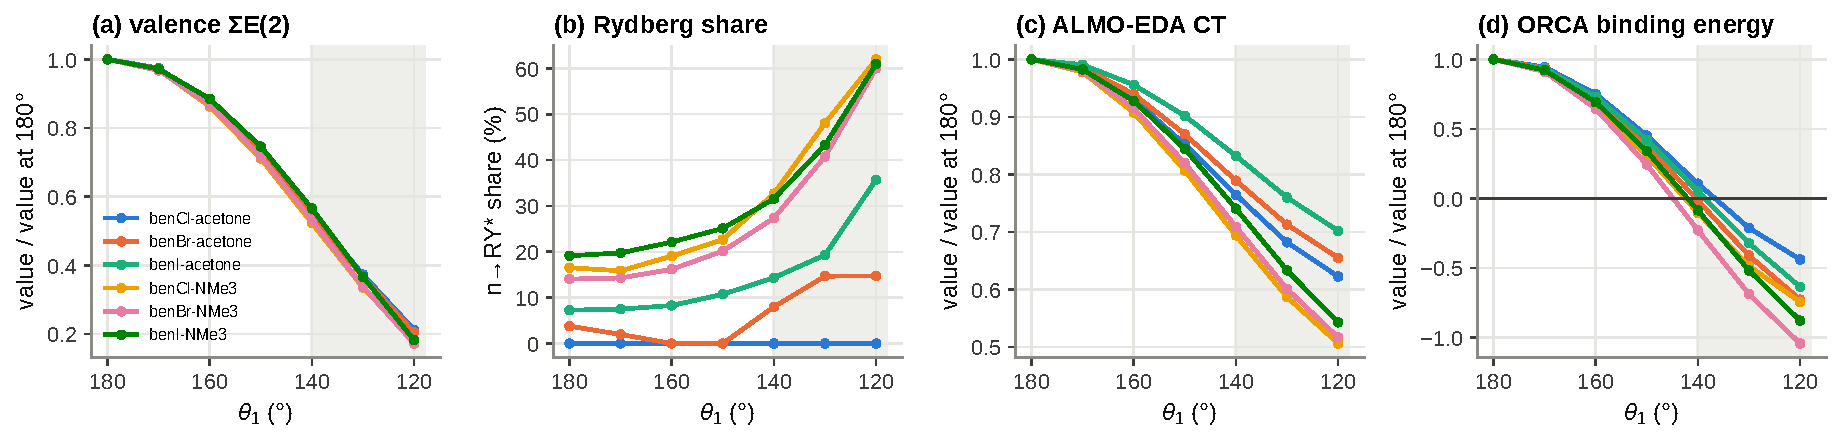
\includegraphics[width=0.85\textwidth]{FigS4_angle_scan_QM.pdf}
\caption{Rigid angle scans relative to the linear contact. (a) Valence $\Sigma\ET$. (b) ALMO-EDA CT energy. (c) ORCA counterpoise binding energy. Shaded range: outside the T1 angle window.}
\label{fig:angqm}
\end{figure}

\begin{figure}[!htbp]
\centering
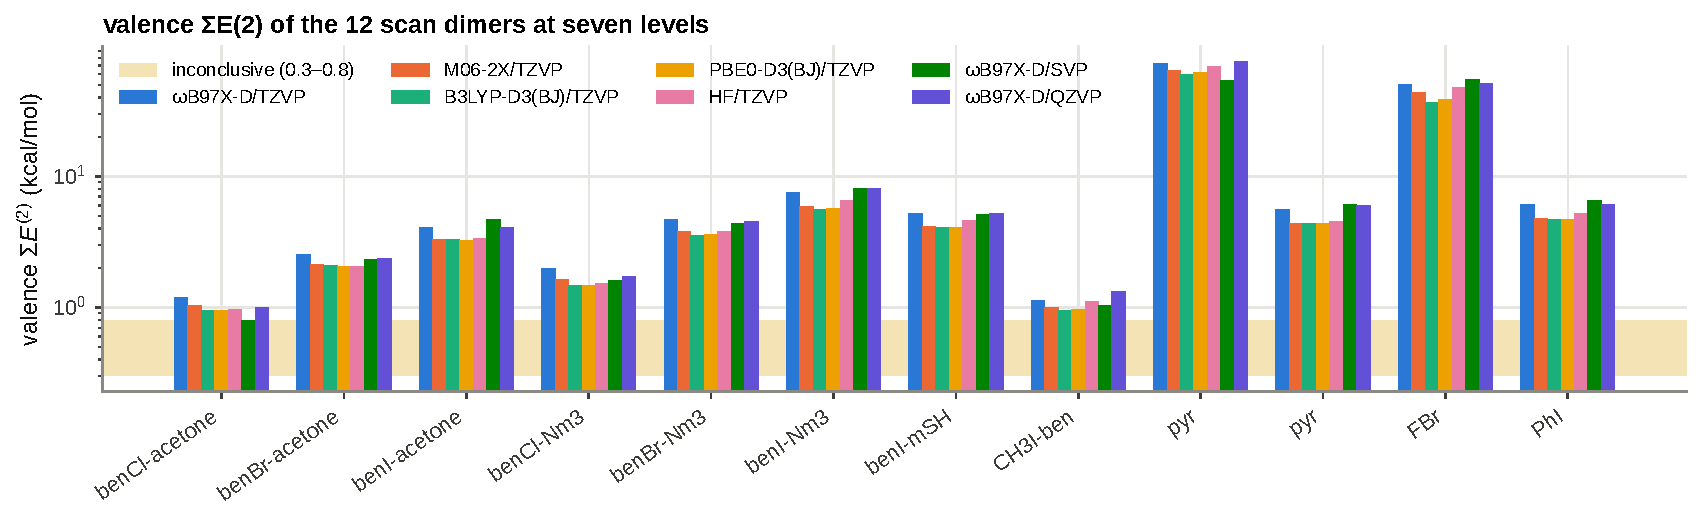
\includegraphics[width=0.85\textwidth]{FigS5_method_basis.pdf}
\caption{Valence $\Sigma\ET$ of the 12 scan dimers at $d_\mathrm{eq}$ at seven levels of theory. Shaded band: grey zone.}
\label{fig:mb}
\end{figure}

% ---- table from tables/tab_levels.tex (generated) ----
\begin{table}[!htbp]\centering\small
\caption{Valence $\Sigma E^{(2)}$ of the 12 scan dimers at $d_\mathrm{eq}$ relative to $\omega$B97X-D/def2-TZVP (Set D, Gaussian~16). No decision changes; the smallest value at any level is 0.80~kcal\,mol$^{-1}$; the rank correlation with the default level is at least 0.98.}\label{tab:levels}
\begin{tabular}{llrr}\toprule Method & Basis & min ratio & max ratio\\\midrule
HF & def2-TZVP & 0.77 & 0.99\\
B3LYP-D3(BJ) & def2-TZVP & 0.74 & 0.85\\
PBE0-D3(BJ) & def2-TZVP & 0.75 & 0.86\\
M06-2X & def2-TZVP & 0.78 & 0.89\\
$\omega$B97X-D & def2-SVP & 0.68 & 1.15\\
$\omega$B97X-D & def2-QZVP & 0.84 & 1.17\\
\bottomrule\end{tabular}\end{table}
% ---- end of tables/tab_levels.tex ----

\begin{figure}[!htbp]
\centering
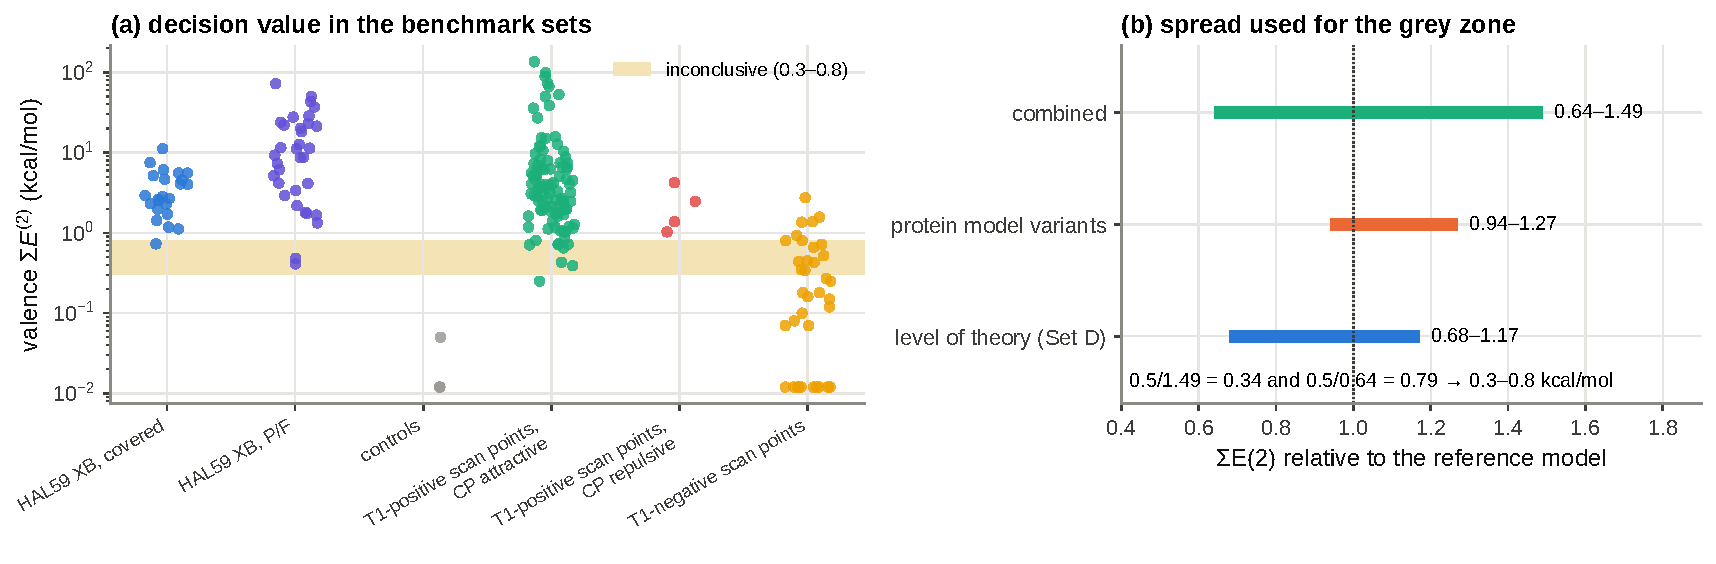
\includegraphics[width=\textwidth]{FigS6_gate_calibration.pdf}
\caption{Calibration of the NBO screen. (a) Valence $\Sigma\ET$ of the HAL59 halogen bonds (covered by T1, and with P or F acceptors), the controls, and the scan points that pass T1 with an attractive or a repulsive counterpoise energy or that fail T1; zeros are drawn at 0.012~kcal\,mol$^{-1}$. (b) Spread of $\Sigma\ET$ over the levels of theory (Set D, ratio to $\omega$B97X-D/def2-TZVP; extremes: chlorobenzene$\cdots$acetone with def2-SVP, 0.68, and CH$_3$I$\cdots$benzene with def2-QZVP, 1.17) and over the protein model variants (ratio to the default PCM cluster; extremes: Asn65 in the gas-phase cluster, 0.94, and Thr113 in QM/MM with the Z3 boundary, 1.27), and their product, which maps the conventional centre of 0.5~kcal\,mol$^{-1}$ onto 0.34--0.79~kcal\,mol$^{-1}$. Without the Thr113 contact, whose model has the hydroxyl artefact, the protein maximum is 1.16 (Phe80, Z1 boundary), and the zone becomes 0.37--0.79~kcal\,mol$^{-1}$; the zone used, 0.3--0.8~kcal\,mol$^{-1}$, covers both.}
\label{fig:gatecal}
\end{figure}

\paragraph{In-cluster pairs.} Table~\ref{tab:pairs} lists every halogen$\cdots$N, O, or S pair within \SI{4.5}{\angstrom} inside the default clusters. The twelve pairs that pass T1 are the target contacts and their chain replicas. The six pairs that fail T1 all have backbone amide N partners and valence values of at most 0.06~kcal\,mol$^{-1}$, but they never reach the screen in the workflow, so they confirm the geometric exclusion and do not test the screen; Section~\ref{sec:hardneg} gives that test.

% ---- table from tables/tab_pairs.tex (generated) ----
\begin{table}[!htbp]\centering\scriptsize\setlength{\tabcolsep}{3pt}
\caption{Every halogen$\cdots$N, O, or S pair within 4.5~\AA{} inside the default PCM cluster models, whether or not it passes T1 (kcal\,mol$^{-1}$). The twelve pairs that pass T1 are the target contacts and their chain replicas. The six pairs that fail T1 never reach the NBO screen in the workflow, so their small values confirm the geometric exclusion rather than test the screen on contacts that pass T1; ESI Table~\ref{tab:hardneg} gives that test. Fail: criterion of T1 that is not met. Base: Lewis base or poor Lewis base. X$\to$Y--H: halogen lone pair into an N--H or O--H antibond on the partner residue.}\label{tab:pairs}
\begin{tabular}{lllrrrllrrr}\toprule PDB & X & Y & $d$ (\AA) & $\theta_1$ & $d_\mathrm{cut}$ & T1 & Base & $\Sigma E^{(2)}$ & RY & X$\to$Y--H\\\midrule
2W0S & Br & N Asn65 (A) & 4.09 & 123.8 & 3.84 & distance, angle & poor & 0.00 & 0.00 & 0.00\\
1P5E & Br11 & N Leu83 (A) & 3.80 & 131.4 & 3.84 & angle & poor & 0.00 & 0.00 & 0.81\\
2W0S & Br & N Asn65 (B) & 4.44 & 115.6 & 3.84 & distance, angle & poor & 0.00 & 0.00 & 0.00\\
1P5E & Br11 & N Leu83 (C) & 3.66 & 131.3 & 3.84 & angle & poor & 0.00 & 0.00 & 1.39\\
1P5E & Br12 & N Leu83 (C) & 3.99 & 119.4 & 3.84 & distance, angle & poor & 0.00 & 0.09 & 0.28\\
1P5E & Br12 & N Leu83 (A) & 3.94 & 124.3 & 3.84 & distance, angle & poor & 0.06 & 0.00 & 0.26\\
4DST & Cl2 & N Gly75 (A) & 3.52 & 140.5 & 3.77 & T1 pass & poor & 0.07 & 0.06 & 0.00\\
1US0 & Br8 & OG1 Thr113 (A) & 2.97 & 152.8 & 3.68 & T1 pass & base & 0.33 & 0.16 & 5.89\\
1P5E & Br10 & O Ile10 (A) & 3.24 & 144.1 & 3.68 & T1 pass & base & 0.33 & 0.00 & 0.00\\
4GQL & Cl1 & O Pro232 (A) & 2.69 & 166.7 & 3.61 & T1 pass & base & 1.87 & 0.06 & 0.00\\
1P5E & Br12 & O Glu81 (C) & 3.05 & 171.7 & 3.68 & T1 pass & base & 1.87 & 0.00 & 0.00\\
2W0S & Br & OD1 Asn65 (B) & 2.82 & 155.9 & 3.68 & T1 pass & base & 2.05 & 0.23 & 0.00\\
4AGL & I15 & O Leu145 (A) & 3.01 & 171.6 & 3.82 & T1 pass & base & 2.07 & 0.13 & 0.00\\
1P5E & Br12 & O Glu81 (A) & 3.01 & 168.5 & 3.68 & T1 pass & base & 2.08 & 0.00 & 0.00\\
4AGL & I15 & O Leu145 (B) & 2.98 & 172.0 & 3.82 & T1 pass & base & 2.30 & 0.10 & 0.00\\
1P5E & Br11 & O Leu83 (C) & 2.88 & 176.9 & 3.68 & T1 pass & base & 3.02 & 0.06 & 0.00\\
1P5E & Br11 & O Leu83 (A) & 2.90 & 164.7 & 3.68 & T1 pass & base & 3.07 & 0.00 & 0.00\\
2W0S & Br & OD1 Asn65 (A) & 2.69 & 168.3 & 3.68 & T1 pass & base & 3.86 & 0.46 & 0.00\\
\bottomrule\end{tabular}\end{table}
% ---- end of tables/tab_pairs.tex ----

\paragraph{Amide N atoms.} In the protein models, 124 backbone and side-chain amide N atoms are intact (bonded to their carbonyl carbon). NBO prints a lone pair on 116 of them, but none donates into $\sigma^*$(C--X) above the print threshold of 0.05~kcal\,mol$^{-1}$ (\texttt{results/v3/amideN\_v3.csv}).

\paragraph{Proteins.} Table~\ref{tab:protcontacts} summarizes the nine contacts and five replicas, Table~\ref{tab:qmprot} gives every model, and Table~\ref{tab:proteda} compares the cluster interaction energies. ORCA and ALMO-EDA share the level of theory and agree within 0.11~kcal\,mol$^{-1}$.

% ---- table from tables/tab_protcontacts.tex (generated) ----
\begin{table}[!htbp]\centering\scriptsize\setlength{\tabcolsep}{2.5pt}
\caption{Electronic tiers for the protein contacts (Gaussian~16, $\omega$B97X-D/def2-TZVP; kcal\,mol$^{-1}$). $n$: number of models. Default: PCM cluster ($\varepsilon=4$). Range: all models (gas, PCM, QM size, and QM/MM variants). RY: $n\to$RY$^*$(X) part in the default model. With RY: valence plus Rydberg sum, and the decision of a rule that counts the Rydberg terms against a single threshold of 0.5~kcal\,mol$^{-1}$ (pass/fail; the published-model Rydberg-inclusive comparison). X$\to$Y--H: summed donation from the halogen lone pairs into the N--H and O--H antibonds of the acceptor residue; X$\to$frag.~2: the same into any N--H or O--H antibond of fragment~2. H-bond flag: models in which X$\to$frag.~2 exceeds $\Sigma E^{(2)}$ (and 0.5~kcal\,mol$^{-1}$). D: decisions over all models. BXQI: from $G$ and the default $\Sigma E^{(2)}$. The set-F models use the template rotamer of the 1US0 Thr113 hydroxyl, whose hydrogen points toward bromine; the alternate oriented-hydrogen models are listed separately in the model column.}\label{tab:protcontacts}
\resizebox{\textwidth}{!}{\begin{tabular}{llrrrlrlllrllr}\toprule PDB & Contact & $n$ & $G$ & $\Sigma E^{(2)}$ & range & RY & with RY & 0.5 rule & X$\to$Y--H & X$\to$frag.~2 & H-bond flag & D & BXQI\\\midrule
2W0S & Br$\cdots$OD1 Asn65 (A) & 14 & 0.87 & 3.86 & 3.61--4.17 & 0.46 & 4.02--4.72 & pass & 0.00 & 10.79 & 2/14 & S & 86.2\\
1P5E & Br11$\cdots$O Leu83 (C) & 1 & 0.97 & 3.02 & 3.02--3.02 & 0.06 & 3.08--3.08 & pass & 0.00 & 1.39 & 0/1 & S & 86.1\\
1P5E & Br11$\cdots$O Leu83 (A) & 14 & 0.83 & 3.07 & 3.07--3.47 & 0.00 & 3.07--3.56 & pass & 0.00 & 1.15 & 0/14 & S & 80.5\\
4AGL & I15$\cdots$O Leu145 (B) & 1 & 0.93 & 2.30 & 2.30--2.30 & 0.10 & 2.40--2.40 & pass & 0.00 & 0.00 & 0/1 & S & 78.6\\
4AGL & I15$\cdots$O Leu145 (A) & 14 & 0.91 & 2.07 & 1.96--2.24 & 0.13 & 2.02--2.30 & pass & 0.00 & 0.44 & 0/14 & S & 75.4\\
4GQL & Cl1$\cdots$O Pro232 (A) & 14 & 0.87 & 1.87 & 1.75--1.96 & 0.06 & 1.83--2.04 & pass & 0.00 & 0.00 & 0/14 & S & 71.5\\
1P5E & Br12$\cdots$O Glu81 (A) & 14 & 0.76 & 2.08 & 2.08--2.33 & 0.00 & 2.08--2.33 & pass & 0.00 & 0.46 & 0/14 & S & 69.6\\
1P5E & Br12$\cdots$O Glu81 (C) & 1 & 0.78 & 1.87 & 1.87--1.87 & 0.00 & 1.87--1.87 & pass & 0.00 & 0.28 & 0/1 & S & 68.1\\
2W0S & Br$\cdots$OD1 Asn65 (B) & 1 & 0.72 & 2.05 & 2.05--2.05 & 0.23 & 2.28--2.28 & pass & 0.00 & 0.00 & 0/1 & S & 67.6\\
1P5E & Br13$\cdots$$\pi$ Phe80 (C) & 1 & 0.54 & 1.31 & 1.31--1.31 & 0.00 & 1.31--1.31 & pass & 0.00 & 0.00 & 0/1 & S & 50.7\\
1P5E & Br13$\cdots$$\pi$ Phe80 (A) & 14 & 0.51 & 0.55 & 0.52--0.64 & 0.00 & 0.52--0.64 & pass & 0.00 & 0.00 & 0/14 & I & 33.8\\
1US0 & Br8$\cdots$OG1 Thr113 (A) & 16 & 0.64 & 0.33 & 0.31--0.42 & 0.16 & 0.38--0.72 & fail/pass & 6.67 & 6.67 & 16/16 & I & 29.2\\
1P5E & Br10$\cdots$O Ile10 (A) & 14 & 0.38 & 0.33 & 0.31--0.36 & 0.00 & 0.31--0.36 & fail & 0.00 & 0.00 & 0/14 & I & 23.1\\
4DST & Cl2$\cdots$N Gly75 (A) & 14 & 0.12 & 0.07 & 0.00--0.07 & 0.06 & 0.00--0.13 & fail & 0.00 & 0.00 & 0/14 & N & 6.1\\
\bottomrule\end{tabular}}\end{table}
% ---- end of tables/tab_protcontacts.tex ----
% ---- table from tables/tab_qm_prot.tex (generated) ----
{\scriptsize
\setlength{\tabcolsep}{3pt}
\begin{longtable}{lllrrrrlrl}
\caption{NBO screen of every protein model (Gaussian~16, $\omega$B97X-D/def2-TZVP; kcal\,mol$^{-1}$). QM/MM models use ff14SB, the RC boundary, and \SI{15}{\angstrom} unless the model name says otherwise. LP(Y): NBO prints a lone pair on the acceptor atom. $\Delta q_\mathrm{CT}$: NPA charge moved to fragment~1 ($10^{-3}$~e); in a protein cluster it sums every ligand--environment contact and is not specific to the halogen bond. D: decision as in Table~\ref{tab:qmhal}.}\label{tab:qmprot}\\
\toprule
PDB & Contact & Model & $\Sigma E^{(2)}$ & RY & X$\to$Y--H & X$\to$frag.~2 & LP(Y) & $\Delta q_\mathrm{CT}$ & D\\
\midrule
\endfirsthead
\toprule
PDB & Contact & Model & $\Sigma E^{(2)}$ & RY & X$\to$Y--H & X$\to$frag.~2 & LP(Y) & $\Delta q_\mathrm{CT}$ & D\\
\midrule
\endhead
\bottomrule
\endlastfoot
1P5E & Br10$\cdots$O Ile10 (A) & cluster, gas & 0.32 & 0.00 & 0.00 & 0.00 & yes & 2.5 & I\\
1P5E & Br10$\cdots$O Ile10 (A) & cluster, PCM & 0.33 & 0.00 & 0.00 & 0.00 & yes & 3.8 & I\\
1P5E & Br10$\cdots$O Ile10 (A) & +3~\AA{} shell & 0.33 & 0.00 & 0.00 & 0.00 & yes & 3.8 & I\\
1P5E & Br10$\cdots$O Ile10 (A) & +4~\AA{} shell & 0.33 & 0.00 & 0.00 & 0.00 & yes & -3.4 & I\\
1P5E & Br10$\cdots$O Ile10 (A) & +5~\AA{} shell & 0.36 & 0.00 & 0.00 & 0.00 & yes & -4.6 & I\\
1P5E & Br10$\cdots$O Ile10 (A) & QM/MM ff14SB & 0.31 & 0.00 & 0.00 & 0.00 & yes & 1.0 & I\\
1P5E & Br10$\cdots$O Ile10 (A) & QM/MM CHARMM36 & 0.32 & 0.00 & 0.00 & 0.00 & yes & 2.4 & I\\
1P5E & Br10$\cdots$O Ile10 (A) & QM/MM Z1 & 0.32 & 0.00 & 0.00 & 0.00 & yes & 8.0 & I\\
1P5E & Br10$\cdots$O Ile10 (A) & QM/MM Z2 & 0.31 & 0.00 & 0.00 & 0.00 & yes & 0.6 & I\\
1P5E & Br10$\cdots$O Ile10 (A) & QM/MM Z3 & 0.32 & 0.00 & 0.00 & 0.00 & yes & 1.8 & I\\
1P5E & Br10$\cdots$O Ile10 (A) & QM/MM 10~\AA{} & 0.32 & 0.00 & 0.00 & 0.00 & yes & 1.5 & I\\
1P5E & Br10$\cdots$O Ile10 (A) & QM/MM 20~\AA{} & 0.31 & 0.00 & 0.00 & 0.00 & yes & -0.9 & I\\
1P5E & Br10$\cdots$O Ile10 (A) & QM/MM 25~\AA{} & 0.31 & 0.00 & 0.00 & 0.00 & yes & -1.9 & I\\
1P5E & Br10$\cdots$O Ile10 (A) & QM/MM whole & 0.31 & 0.00 & 0.00 & 0.00 & yes & -2.8 & I\\
1P5E & Br11$\cdots$O Leu83 (A) & cluster, gas & 3.07 & 0.00 & 0.00 & 0.79 & yes & 2.5 & S\\
1P5E & Br11$\cdots$O Leu83 (A) & cluster, PCM & 3.07 & 0.00 & 0.00 & 0.81 & yes & 3.8 & S\\
1P5E & Br11$\cdots$O Leu83 (A) & +3~\AA{} shell & 3.07 & 0.00 & 0.00 & 0.81 & yes & 3.8 & S\\
1P5E & Br11$\cdots$O Leu83 (A) & +4~\AA{} shell & 3.10 & 0.06 & 0.00 & 0.81 & yes & -3.4 & S\\
1P5E & Br11$\cdots$O Leu83 (A) & +5~\AA{} shell & 3.11 & 0.07 & 0.00 & 1.15 & yes & -4.6 & S\\
1P5E & Br11$\cdots$O Leu83 (A) & QM/MM ff14SB & 3.24 & 0.07 & 0.00 & 0.83 & yes & 1.0 & S\\
1P5E & Br11$\cdots$O Leu83 (A) & QM/MM CHARMM36 & 3.18 & 0.00 & 0.00 & 0.84 & yes & 2.4 & S\\
1P5E & Br11$\cdots$O Leu83 (A) & QM/MM Z1 & 3.14 & 0.00 & 0.00 & 0.72 & yes & 8.0 & S\\
1P5E & Br11$\cdots$O Leu83 (A) & QM/MM Z2 & 3.10 & 0.06 & 0.00 & 0.80 & yes & 0.6 & S\\
1P5E & Br11$\cdots$O Leu83 (A) & QM/MM Z3 & 3.47 & 0.09 & 0.00 & 0.81 & yes & 1.8 & S\\
1P5E & Br11$\cdots$O Leu83 (A) & QM/MM 10~\AA{} & 3.08 & 0.00 & 0.00 & 0.87 & yes & 1.5 & S\\
1P5E & Br11$\cdots$O Leu83 (A) & QM/MM 20~\AA{} & 3.11 & 0.00 & 0.00 & 0.86 & yes & -0.9 & S\\
1P5E & Br11$\cdots$O Leu83 (A) & QM/MM 25~\AA{} & 3.10 & 0.00 & 0.00 & 0.86 & yes & -1.9 & S\\
1P5E & Br11$\cdots$O Leu83 (A) & QM/MM whole & 3.11 & 0.06 & 0.00 & 0.86 & yes & -2.8 & S\\
1P5E & Br12$\cdots$O Glu81 (A) & cluster, gas & 2.11 & 0.00 & 0.00 & 0.26 & yes & 2.5 & S\\
1P5E & Br12$\cdots$O Glu81 (A) & cluster, PCM & 2.08 & 0.00 & 0.00 & 0.26 & yes & 3.8 & S\\
1P5E & Br12$\cdots$O Glu81 (A) & +3~\AA{} shell & 2.08 & 0.00 & 0.00 & 0.26 & yes & 3.8 & S\\
1P5E & Br12$\cdots$O Glu81 (A) & +4~\AA{} shell & 2.14 & 0.00 & 0.00 & 0.26 & yes & -3.4 & S\\
1P5E & Br12$\cdots$O Glu81 (A) & +5~\AA{} shell & 2.33 & 0.00 & 0.00 & 0.46 & yes & -4.6 & S\\
1P5E & Br12$\cdots$O Glu81 (A) & QM/MM ff14SB & 2.24 & 0.00 & 0.00 & 0.28 & yes & 1.0 & S\\
1P5E & Br12$\cdots$O Glu81 (A) & QM/MM CHARMM36 & 2.25 & 0.00 & 0.00 & 0.28 & yes & 2.4 & S\\
1P5E & Br12$\cdots$O Glu81 (A) & QM/MM Z1 & 2.28 & 0.00 & 0.00 & 0.24 & yes & 8.0 & S\\
1P5E & Br12$\cdots$O Glu81 (A) & QM/MM Z2 & 2.18 & 0.00 & 0.00 & 0.26 & yes & 0.6 & S\\
1P5E & Br12$\cdots$O Glu81 (A) & QM/MM Z3 & 2.09 & 0.00 & 0.00 & 0.25 & yes & 1.8 & S\\
1P5E & Br12$\cdots$O Glu81 (A) & QM/MM 10~\AA{} & 2.21 & 0.00 & 0.00 & 0.29 & yes & 1.5 & S\\
1P5E & Br12$\cdots$O Glu81 (A) & QM/MM 20~\AA{} & 2.17 & 0.00 & 0.00 & 0.29 & yes & -0.9 & S\\
1P5E & Br12$\cdots$O Glu81 (A) & QM/MM 25~\AA{} & 2.15 & 0.00 & 0.00 & 0.30 & yes & -1.9 & S\\
1P5E & Br12$\cdots$O Glu81 (A) & QM/MM whole & 2.16 & 0.00 & 0.00 & 0.29 & yes & -2.8 & S\\
1P5E & Br13$\cdots$$\pi$ Phe80 (A) & cluster, gas & 0.53 & 0.00 & 0.00 & 0.00 & no & 2.5 & I\\
1P5E & Br13$\cdots$$\pi$ Phe80 (A) & cluster, PCM & 0.55 & 0.00 & 0.00 & 0.00 & no & 3.8 & I\\
1P5E & Br13$\cdots$$\pi$ Phe80 (A) & +3~\AA{} shell & 0.55 & 0.00 & 0.00 & 0.00 & no & 3.8 & I\\
1P5E & Br13$\cdots$$\pi$ Phe80 (A) & +4~\AA{} shell & 0.57 & 0.00 & 0.00 & 0.00 & no & -3.4 & I\\
1P5E & Br13$\cdots$$\pi$ Phe80 (A) & +5~\AA{} shell & 0.58 & 0.00 & 0.00 & 0.00 & no & -4.6 & I\\
1P5E & Br13$\cdots$$\pi$ Phe80 (A) & QM/MM ff14SB & 0.58 & 0.00 & 0.00 & 0.00 & no & 1.0 & I\\
1P5E & Br13$\cdots$$\pi$ Phe80 (A) & QM/MM CHARMM36 & 0.59 & 0.00 & 0.00 & 0.00 & no & 2.4 & I\\
1P5E & Br13$\cdots$$\pi$ Phe80 (A) & QM/MM Z1 & 0.64 & 0.00 & 0.00 & 0.00 & no & 8.0 & I\\
1P5E & Br13$\cdots$$\pi$ Phe80 (A) & QM/MM Z2 & 0.58 & 0.00 & 0.00 & 0.00 & no & 0.6 & I\\
1P5E & Br13$\cdots$$\pi$ Phe80 (A) & QM/MM Z3 & 0.52 & 0.00 & 0.00 & 0.00 & no & 1.8 & I\\
1P5E & Br13$\cdots$$\pi$ Phe80 (A) & QM/MM 10~\AA{} & 0.59 & 0.00 & 0.00 & 0.00 & no & 1.5 & I\\
1P5E & Br13$\cdots$$\pi$ Phe80 (A) & QM/MM 20~\AA{} & 0.57 & 0.00 & 0.00 & 0.00 & no & -0.9 & I\\
1P5E & Br13$\cdots$$\pi$ Phe80 (A) & QM/MM 25~\AA{} & 0.57 & 0.00 & 0.00 & 0.00 & no & -1.9 & I\\
1P5E & Br13$\cdots$$\pi$ Phe80 (A) & QM/MM whole & 0.57 & 0.00 & 0.00 & 0.00 & no & -2.8 & I\\
1P5E & Br11$\cdots$O Leu83 (C) & cluster, PCM & 3.02 & 0.06 & 0.00 & 1.39 & yes & 16.6 & S\\
1P5E & Br12$\cdots$O Glu81 (C) & cluster, PCM & 1.87 & 0.00 & 0.00 & 0.28 & yes & 16.6 & S\\
1P5E & Br13$\cdots$$\pi$ Phe80 (C) & cluster, PCM & 1.31 & 0.00 & 0.00 & 0.00 & no & 16.6 & S\\
1US0 & Br8$\cdots$OG1 Thr113 (A) & cluster, gas & 0.31 & 0.15 & 6.19 & 6.19 & yes & -8.6 & I\\
1US0 & Br8$\cdots$OG1 Thr113 (A) & cluster, PCM & 0.33 & 0.16 & 5.89 & 5.89 & yes & -6.7 & I\\
1US0 & Br8$\cdots$OG1 Thr113 (A) & +3~\AA{} shell & 0.33 & 0.16 & 5.89 & 5.89 & yes & -6.7 & I\\
1US0 & Br8$\cdots$OG1 Thr113 (A) & +4~\AA{} shell & 0.32 & 0.06 & 6.67 & 6.67 & yes & -18.7 & I\\
1US0 & Br8$\cdots$OG1 Thr113 (A) & +5~\AA{} shell & 0.32 & 0.06 & 6.64 & 6.64 & yes & -17.9 & I\\
1US0 & Br8$\cdots$OG1 Thr113 (A) & QM/MM ff14SB & 0.37 & 0.26 & 5.38 & 5.38 & yes & -2.5 & I\\
1US0 & Br8$\cdots$OG1 Thr113 (A) & QM/MM CHARMM36 & 0.37 & 0.26 & 5.38 & 5.38 & yes & -2.1 & I\\
1US0 & Br8$\cdots$OG1 Thr113 (A) & QM/MM Z1 & 0.41 & 0.30 & 4.95 & 4.95 & yes & 1.6 & I\\
1US0 & Br8$\cdots$OG1 Thr113 (A) & QM/MM Z2 & 0.37 & 0.25 & 5.34 & 5.34 & yes & -2.1 & I\\
1US0 & Br8$\cdots$OG1 Thr113 (A) & QM/MM Z3 & 0.42 & 0.30 & 5.02 & 5.02 & yes & 0.5 & I\\
1US0 & Br8$\cdots$OG1 Thr113 (A) & QM/MM 10~\AA{} & 0.37 & 0.25 & 5.42 & 5.42 & yes & -2.6 & I\\
1US0 & Br8$\cdots$OG1 Thr113 (A) & QM/MM 20~\AA{} & 0.38 & 0.26 & 5.32 & 5.32 & yes & -2.1 & I\\
1US0 & Br8$\cdots$OG1 Thr113 (A) & QM/MM 25~\AA{} & 0.38 & 0.27 & 5.31 & 5.31 & yes & -2.0 & I\\
1US0 & Br8$\cdots$OG1 Thr113 (A) & QM/MM whole & 0.38 & 0.26 & 5.31 & 5.31 & yes & -2.1 & I\\
1US0 & Br8$\cdots$OG1 Thr113 (A) & QM/MM His110 HID & 0.37 & 0.24 & 5.45 & 5.45 & yes & -2.8 & I\\
1US0 & Br8$\cdots$OG1 Thr113 (A) & QM/MM His110 HIP & 0.38 & 0.26 & 5.26 & 5.26 & yes & -1.4 & I\\
2W0S & Br$\cdots$OD1 Asn65 (A) & cluster, gas & 3.61 & 0.41 & 0.00 & 0.00 & yes & 4.0 & S\\
2W0S & Br$\cdots$OD1 Asn65 (A) & cluster, PCM & 3.86 & 0.46 & 0.00 & 0.00 & yes & 8.4 & S\\
2W0S & Br$\cdots$OD1 Asn65 (A) & +3~\AA{} shell & 3.86 & 0.46 & 0.00 & 0.00 & yes & 8.4 & S\\
2W0S & Br$\cdots$OD1 Asn65 (A) & +4~\AA{} shell & 4.09 & 0.43 & 0.00 & 10.79 & yes & -30.8 & S\\
2W0S & Br$\cdots$OD1 Asn65 (A) & +5~\AA{} shell & 4.11 & 0.38 & 0.00 & 10.61 & yes & -26.6 & S\\
2W0S & Br$\cdots$OD1 Asn65 (A) & QM/MM ff14SB & 4.11 & 0.51 & 0.00 & 0.00 & yes & 11.0 & S\\
2W0S & Br$\cdots$OD1 Asn65 (A) & QM/MM CHARMM36 & 4.11 & 0.51 & 0.00 & 0.00 & yes & 10.9 & S\\
2W0S & Br$\cdots$OD1 Asn65 (A) & QM/MM Z1 & 4.17 & 0.55 & 0.00 & 0.00 & yes & 12.4 & S\\
2W0S & Br$\cdots$OD1 Asn65 (A) & QM/MM Z2 & 4.13 & 0.52 & 0.00 & 0.00 & yes & 11.4 & S\\
2W0S & Br$\cdots$OD1 Asn65 (A) & QM/MM Z3 & 4.17 & 0.54 & 0.00 & 0.00 & yes & 12.5 & S\\
2W0S & Br$\cdots$OD1 Asn65 (A) & QM/MM 10~\AA{} & 3.98 & 0.49 & 0.00 & 0.00 & yes & 9.0 & S\\
2W0S & Br$\cdots$OD1 Asn65 (A) & QM/MM 20~\AA{} & 4.07 & 0.50 & 0.00 & 0.00 & yes & 10.3 & S\\
2W0S & Br$\cdots$OD1 Asn65 (A) & QM/MM 25~\AA{} & 4.00 & 0.49 & 0.00 & 0.00 & yes & 9.1 & S\\
2W0S & Br$\cdots$OD1 Asn65 (A) & QM/MM whole & 3.99 & 0.49 & 0.00 & 0.00 & yes & 9.0 & S\\
2W0S & Br$\cdots$OD1 Asn65 (B) & cluster, PCM & 2.05 & 0.23 & 0.00 & 0.00 & yes & 5.2 & S\\
4AGL & I15$\cdots$O Leu145 (A) & cluster, gas & 2.05 & 0.08 & 0.00 & 0.00 & yes & 9.4 & S\\
4AGL & I15$\cdots$O Leu145 (A) & cluster, PCM & 2.07 & 0.13 & 0.00 & 0.00 & yes & 10.3 & S\\
4AGL & I15$\cdots$O Leu145 (A) & +3~\AA{} shell & 2.07 & 0.13 & 0.00 & 0.00 & yes & 10.3 & S\\
4AGL & I15$\cdots$O Leu145 (A) & +4~\AA{} shell & 2.13 & 0.15 & 0.00 & 0.25 & yes & -7.8 & S\\
4AGL & I15$\cdots$O Leu145 (A) & +5~\AA{} shell & 2.24 & 0.06 & 0.00 & 0.44 & yes & -10.6 & S\\
4AGL & I15$\cdots$O Leu145 (A) & QM/MM ff14SB & 2.05 & 0.07 & 0.00 & 0.00 & yes & 8.8 & S\\
4AGL & I15$\cdots$O Leu145 (A) & QM/MM CHARMM36 & 2.05 & 0.07 & 0.00 & 0.00 & yes & 9.1 & S\\
4AGL & I15$\cdots$O Leu145 (A) & QM/MM Z1 & 2.11 & 0.08 & 0.00 & 0.00 & yes & 11.8 & S\\
4AGL & I15$\cdots$O Leu145 (A) & QM/MM Z2 & 2.03 & 0.07 & 0.00 & 0.00 & yes & 9.0 & S\\
4AGL & I15$\cdots$O Leu145 (A) & QM/MM Z3 & 2.09 & 0.08 & 0.00 & 0.00 & yes & 10.3 & S\\
4AGL & I15$\cdots$O Leu145 (A) & QM/MM 10~\AA{} & 2.03 & 0.07 & 0.00 & 0.00 & yes & 8.5 & S\\
4AGL & I15$\cdots$O Leu145 (A) & QM/MM 20~\AA{} & 2.01 & 0.07 & 0.00 & 0.00 & yes & 7.9 & S\\
4AGL & I15$\cdots$O Leu145 (A) & QM/MM 25~\AA{} & 2.01 & 0.07 & 0.00 & 0.00 & yes & 7.9 & S\\
4AGL & I15$\cdots$O Leu145 (A) & QM/MM whole & 1.96 & 0.06 & 0.00 & 0.00 & yes & 6.4 & S\\
4AGL & I15$\cdots$O Leu145 (B) & cluster, PCM & 2.30 & 0.10 & 0.00 & 0.00 & yes & 10.7 & S\\
4DST & Cl2$\cdots$N Gly75 (A) & cluster, gas & 0.07 & 0.05 & 0.00 & 0.00 & yes & 3.7 & N\\
4DST & Cl2$\cdots$N Gly75 (A) & cluster, PCM & 0.07 & 0.06 & 0.00 & 0.00 & yes & 3.9 & N\\
4DST & Cl2$\cdots$N Gly75 (A) & +3~\AA{} shell & 0.07 & 0.06 & 0.00 & 0.00 & yes & 3.9 & N\\
4DST & Cl2$\cdots$N Gly75 (A) & +4~\AA{} shell & 0.00 & 0.00 & 0.00 & 0.00 & yes & -5.7 & N\\
4DST & Cl2$\cdots$N Gly75 (A) & +5~\AA{} shell & 0.00 & 0.00 & 0.00 & 0.00 & yes & -7.6 & N\\
4DST & Cl2$\cdots$N Gly75 (A) & QM/MM ff14SB & 0.06 & 0.00 & 0.00 & 0.00 & yes & 1.2 & N\\
4DST & Cl2$\cdots$N Gly75 (A) & QM/MM CHARMM36 & 0.06 & 0.00 & 0.00 & 0.00 & yes & 0.7 & N\\
4DST & Cl2$\cdots$N Gly75 (A) & QM/MM Z1 & 0.06 & 0.00 & 0.00 & 0.00 & yes & 2.8 & N\\
4DST & Cl2$\cdots$N Gly75 (A) & QM/MM Z2 & 0.06 & 0.00 & 0.00 & 0.00 & yes & 0.9 & N\\
4DST & Cl2$\cdots$N Gly75 (A) & QM/MM Z3 & 0.06 & 0.00 & 0.00 & 0.00 & yes & 2.3 & N\\
4DST & Cl2$\cdots$N Gly75 (A) & QM/MM 10~\AA{} & 0.06 & 0.00 & 0.00 & 0.00 & yes & 0.5 & N\\
4DST & Cl2$\cdots$N Gly75 (A) & QM/MM 20~\AA{} & 0.06 & 0.00 & 0.00 & 0.00 & yes & 1.2 & N\\
4DST & Cl2$\cdots$N Gly75 (A) & QM/MM 25~\AA{} & 0.06 & 0.00 & 0.00 & 0.00 & yes & 0.3 & N\\
4DST & Cl2$\cdots$N Gly75 (A) & QM/MM whole & 0.06 & 0.00 & 0.00 & 0.00 & yes & 0.3 & N\\
4GQL & Cl1$\cdots$O Pro232 (A) & cluster, gas & 1.77 & 0.07 & 0.00 & 0.00 & yes & 3.2 & S\\
4GQL & Cl1$\cdots$O Pro232 (A) & cluster, PCM & 1.87 & 0.06 & 0.00 & 0.00 & yes & 4.6 & S\\
4GQL & Cl1$\cdots$O Pro232 (A) & +3~\AA{} shell & 1.95 & 0.07 & 0.00 & 0.00 & yes & 2.7 & S\\
4GQL & Cl1$\cdots$O Pro232 (A) & +4~\AA{} shell & 1.96 & 0.08 & 0.00 & 0.00 & yes & 10.5 & S\\
4GQL & Cl1$\cdots$O Pro232 (A) & +5~\AA{} shell & 1.96 & 0.08 & 0.00 & 0.00 & yes & 13.5 & S\\
4GQL & Cl1$\cdots$O Pro232 (A) & QM/MM ff14SB & 1.87 & 0.08 & 0.00 & 0.00 & yes & 4.3 & S\\
4GQL & Cl1$\cdots$O Pro232 (A) & QM/MM CHARMM36 & 1.86 & 0.08 & 0.00 & 0.00 & yes & 4.1 & S\\
4GQL & Cl1$\cdots$O Pro232 (A) & QM/MM Z1 & 1.82 & 0.07 & 0.00 & 0.00 & yes & 3.8 & S\\
4GQL & Cl1$\cdots$O Pro232 (A) & QM/MM Z2 & 1.80 & 0.07 & 0.00 & 0.00 & yes & 2.4 & S\\
4GQL & Cl1$\cdots$O Pro232 (A) & QM/MM Z3 & 1.75 & 0.08 & 0.00 & 0.00 & yes & 3.1 & S\\
4GQL & Cl1$\cdots$O Pro232 (A) & QM/MM 10~\AA{} & 1.86 & 0.08 & 0.00 & 0.00 & yes & 4.1 & S\\
4GQL & Cl1$\cdots$O Pro232 (A) & QM/MM 20~\AA{} & 1.89 & 0.07 & 0.00 & 0.00 & yes & 4.4 & S\\
4GQL & Cl1$\cdots$O Pro232 (A) & QM/MM 25~\AA{} & 1.90 & 0.07 & 0.00 & 0.00 & yes & 4.7 & S\\
4GQL & Cl1$\cdots$O Pro232 (A) & QM/MM whole & 1.90 & 0.07 & 0.00 & 0.00 & yes & 4.7 & S\\
\end{longtable}}
% ---- end of tables/tab_qm_prot.tex ----
% ---- table from tables/tab_proteda.tex (generated) ----
\begin{table}[!htbp]\centering\small
\caption{ALMO-EDA of the six finished protein-cluster jobs (Q-Chem~6.2.2, $\omega$B97X-V/def2-TZVPD, gas phase; kcal\,mol$^{-1}$) with the counterpoise interaction energies from ORCA (same level) and Gaussian~16 ($\omega$B97X-D/def2-TZVP, no diffuse functions). The terms cover every contact between the ligand and the acceptor fragment. The large Gaussian--ORCA gap for 2W0S (ligand charge $-2$) shows the need for diffuse functions on anions. Three EDA jobs (2W0S chain A, 1P5E chain A, and 4GQL) stopped during the fragment calculations and gave no result; the 4GQL ORCA job was not run.}\label{tab:proteda}
\begin{tabular}{llrrrrrrr}\toprule PDB & Ligand & FRZ & POL & CT & Total & $\chi_\mathrm{CT}$ & ORCA & G16\\\midrule
1US0 & LDT (A) & 6.98 & -1.27 & -2.36 & 3.35 & 0.65 & 3.38 & 3.85\\
4AGL & P84 (A) & -1.17 & -1.18 & -1.00 & -3.35 & 0.46 & -3.33 & -2.96\\
4DST & 9LI (A) & 0.42 & -0.18 & -0.57 & -0.33 & 0.77 & -0.32 & 0.06\\
2W0S & BVP (B) & 5.19 & -1.24 & -0.91 & 3.04 & 0.42 & 3.07 & 7.75\\
1P5E & TBS (C) & -5.18 & -2.81 & -2.58 & -10.57 & 0.48 & -10.46 & -8.97\\
4AGL & P84 (B) & -0.83 & -1.26 & -1.08 & -3.17 & 0.46 & -3.15 & -2.76\\
\bottomrule\end{tabular}\end{table}
% ---- end of tables/tab_proteda.tex ----

\subsection*{Contacts that pass T1 with poor Lewis bases}
\label{sec:hardneg}
Set G takes single frames from the hIYD release windows in which the T1 acceptor is a poor Lewis base, and five frames with Lewis-base acceptors as controls (Table~\ref{tab:hardneg} and Figure~\ref{fig:classes}b). The cluster models were built with the defaults of \BX{}, so backbone N acceptors keep their amide (two heavy-atom neighbours and one hydrogen on every such N), and they carry the I-Tyr phenolate (charge $-1$) in CPCM ($\varepsilon=4$) at the protein level, $\omega$B97X-D/def2-TZVP. Set J rebuilds the 4DST contact with the amide of Gly75 intact. Of the twelve hIYD contacts with poor Lewis bases, seven are not supported, three are inconclusive with a dominant competing hydrogen bond, and two are supported (Arg164 NH1, 1.47~kcal\,mol$^{-1}$, and the backbone N of Thr178, 0.94~kcal\,mol$^{-1}$); the 4DST contact is not supported in any of its three models (0.00~kcal\,mol$^{-1}$). Four of the five controls are supported (0.91--1.37~kcal\,mol$^{-1}$), and the backbone O of Thr178 is inconclusive (0.69~kcal\,mol$^{-1}$). In the set-G models, the phenolate O of I-Tyr donates 0.65--0.87~kcal\,mol$^{-1}$ into $\sigma^*$(C--I) of its own ring; this intramolecular term does not count. Two further job sets of the repository gave no results and are not used: set H (the marginal protein contacts at five levels), whose route lines repeated keywords so that every job stopped in its first link, and set I (1US0 with NADP$^+$), which was not built.

% ---- table from tables/tab_hardneg.tex (generated) ----
\begin{table}[!htbp]\centering\scriptsize\setlength{\tabcolsep}{2.6pt}
\caption{Contacts that pass T1 but involve poor Lewis bases (hard negatives), with Lewis-base controls from the same simulations (kcal\,mol$^{-1}$). hIYD rows: one frame of a release window each, cluster models built with intact amides and the saved hydroxyl-hydrogen orientations, I-Tyr phenolate charge $-1$, CPCM $\varepsilon=4$, $\omega$B97X-D/def2-TZVP (Gaussian~16, NBO~3.1); every output matched its manifest. 4DST rows: the Cl$\cdots$N Gly75 contact with the amide of Gly75 intact (gas cluster, PCM cluster, QM/MM). Base: Lewis base or poor Lewis base. X$\to$H: summed donation from the iodine lone pairs into the N--H and O--H antibonds of fragment~2. D: decision; $^\dagger$: the competing hydrogen bond exceeds $\Sigma E^{(2)}$.}\label{tab:hardneg}
\resizebox{\textwidth}{!}{\begin{tabular}{lllcrrrrrrrrll}\toprule Residue & Acceptor & Base & Path & $\xi$ & Frame & $d$ & $\theta_1$ & $G$ & $\Sigma E^{(2)}$ & RY & X$\to$H & LP(Y) & D\\\midrule
Lys174 & Lys ammonium NZ & poor & B & 14.8 & 83 & 3.94 & 144.3 & 0.14 & 0.00 & 0.00 & 0.00 & no & N\\
Lys208* & Lys ammonium NZ & poor & B & 14.8 & 1 & 3.90 & 152.6 & 0.24 & 0.00 & 0.00 & 0.06 & no & N\\
Gly166 & backbone amide N & poor & B & 17.8 & 9 & 3.45 & 169.6 & 0.64 & 0.07 & 0.00 & 0.50 & yes & N$^\dagger$\\
Trp169 & Trp indole NE1 & poor & A & 17.8 & 96 & 3.89 & 169.5 & 0.32 & 0.08 & 0.00 & 0.00 & yes & N\\
Arg164 & Arg guanidinium NE & poor & C & 11.8 & 92 & 3.61 & 169.8 & 0.56 & 0.10 & 0.00 & 0.00 & yes & N\\
Asn242 & Asn amide ND2 & poor & A & 10.8 & 96 & 3.83 & 152.6 & 0.34 & 0.14 & 0.14 & 0.12 & yes & N\\
Asn213* & Asn amide ND2 & poor & A & 17.8 & 36 & 3.59 & 153.6 & 0.46 & 0.28 & 0.08 & 0.28 & yes & N\\
Leu259 & backbone amide N & poor & A & 16.8 & 44 & 3.49 & 172.1 & 0.72 & 0.50 & 0.10 & 1.99 & yes & I$^\dagger$\\
Arg177 & Arg guanidinium NH2 & poor & C & 18.8 & 85 & 3.44 & 168.5 & 0.72 & 0.58 & 0.19 & 3.47 & yes & I$^\dagger$\\
Ala130* & backbone amide N & poor & B & 8.8 & 97 & 3.46 & 168.0 & 0.70 & 0.63 & 0.19 & 1.38 & yes & I$^\dagger$\\
Thr178 & backbone amide N & poor & C & 15.8 & 49 & 3.53 & 178.1 & 0.70 & 0.94 & 0.13 & 0.00 & yes & S\\
Arg164 & Arg guanidinium NH1 & poor & C & 11.8 & 91 & 3.31 & 173.8 & 0.77 & 1.47 & 0.30 & 0.00 & yes & S\\
Thr178 & backbone C=O & base & C & 15.8 & 98 & 3.18 & 166.1 & 0.74 & 0.69 & 0.00 & 0.00 & yes & I\\
Asn160 & Asn amide O & base & A & 12.8 & 13 & 3.45 & 166.9 & 0.64 & 0.91 & 0.00 & 0.00 & yes & S\\
Tyr211* & Tyr hydroxyl O & base & B & 16.8 & 9 & 3.41 & 170.0 & 0.69 & 1.08 & 0.00 & 0.00 & yes & S\\
Met165 & Met thioether S & base & C & 17.8 & 46 & 3.90 & 142.6 & 0.24 & 1.15 & 0.23 & 0.00 & yes & S\\
Leu259 & backbone C=O & base & A & 16.8 & 95 & 3.42 & 176.4 & 0.74 & 1.37 & 0.00 & 0.12 & yes & S\\
\midrule
Gly75 (4DST, gas) & backbone amide N & poor & -- & -- & -- & 3.52 & 140.5 & 0.12 & 0.00 & 0.00 & 0.00 & yes & N\\
Gly75 (4DST, PCM) & backbone amide N & poor & -- & -- & -- & 3.52 & 140.5 & 0.12 & 0.00 & 0.00 & 0.00 & yes & N\\
Gly75 (4DST, QM/MM) & backbone amide N & poor & -- & -- & -- & 3.52 & 140.5 & 0.12 & 0.00 & 0.00 & 0.00 & yes & N\\
\bottomrule\end{tabular}}\end{table}
% ---- end of tables/tab_hardneg.tex ----

\begin{figure}[!htbp]
\centering
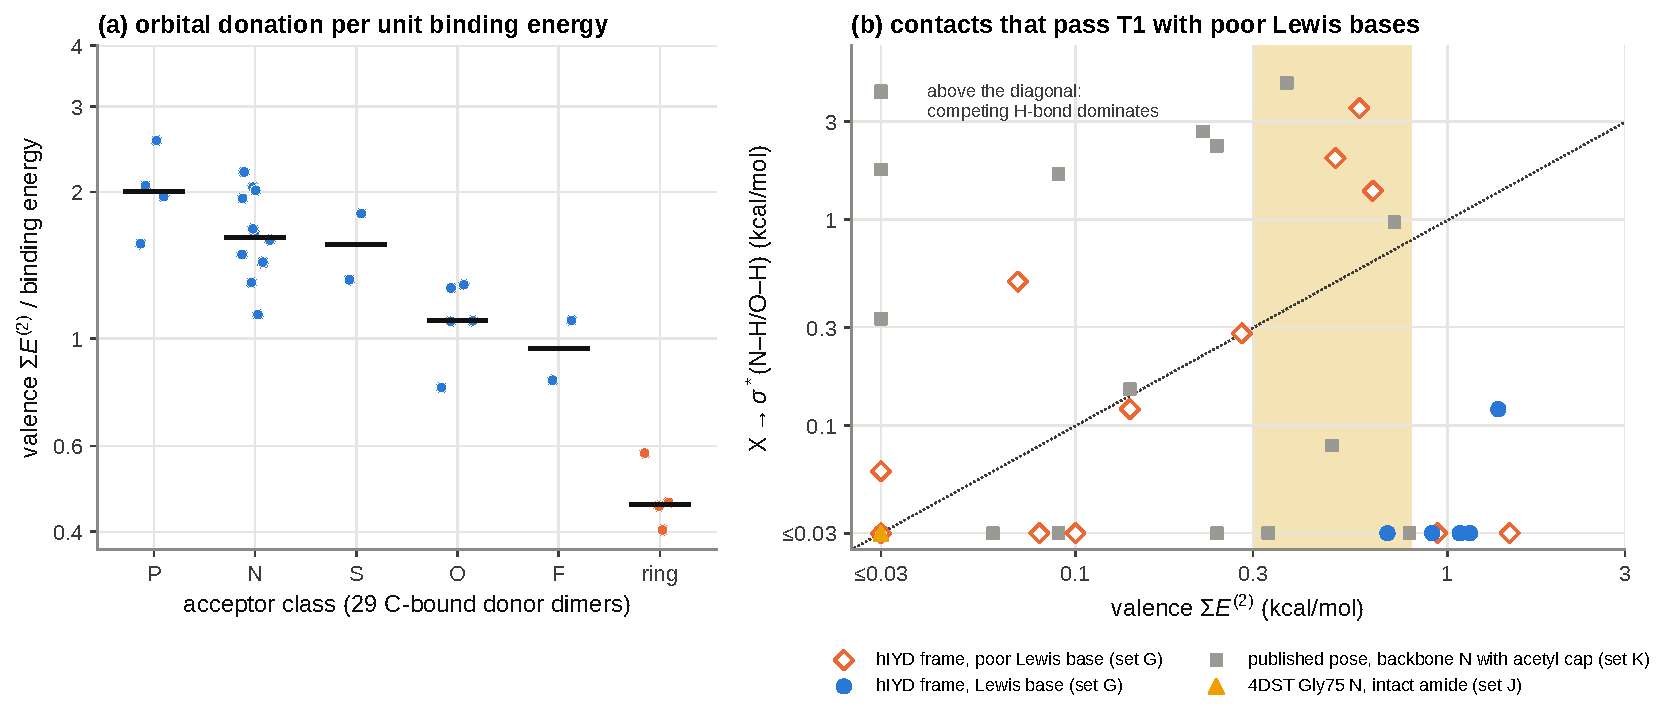
\includegraphics[width=\textwidth]{FigS12_classes_hardneg.pdf}
\caption{(a) Valence $\Sigma\ET$ per unit CCSD(T)/CBS binding energy for the acceptor classes of HAL59 (bars: medians). (b) Contacts that pass T1 with poor Lewis bases: hIYD frames of set G (open diamonds; filled circles: Lewis-base controls), the published hIYD backbone-N poses with the amide restored by an acetyl cap (set K, squares), and 4DST with the amide of Gly75 intact (set J, triangle), plotted as the summed X$\to\sigma^*$(N--H/O--H) donation against $\Sigma\ET$; above the dotted diagonal, the competing hydrogen bond dominates; shaded: grey zone.}
\label{fig:classes}
\end{figure}

%% =====================================================================
\section{Counterpoise Energies from ORCA}
\label{sec:cp}

ORCA~5.0.1 ran 591 single points for sets A--C ($\omega$B97X-V/def2-TZVPD, RIJCOSX, def2/J). Each counterpoise energy uses three jobs: the dimer and each fragment with the ghost basis of the other. Every job terminated normally, and every electron count matched the real atoms. Table~\ref{tab:cpstat} gives the error statistics, Table~\ref{tab:cphal} lists the dimers, and Tables~\ref{tab:cpdist} and~\ref{tab:cpangle} give the scans. ORCA also ran 24 single points for eight protein clusters (Table~\ref{tab:cpprot}) with DefGrid3 and an overlap threshold of $10^{-6}$; the 4GQL cluster was not run.

% ---- table from tables/tab_cp_stats.tex (generated) ----
\begin{table}[!htbp]\centering\footnotesize
\caption{Error statistics of the ORCA counterpoise binding energies against CCSD(T)/CBS (kcal\,mol$^{-1}$). MSE: mean signed error. MAE: mean absolute error. MaxAE: largest absolute error. The I row includes the control FI$\cdots$FCCH. The two fluoroarene controls enter only the first and the last-but-one rows.}\label{tab:cpstat}
\begin{tabular}{lrrrrrrr}\toprule Group & $n$ & MSE & MAE & RMSD & MaxAE & $r$ & $\rho$\\\midrule
All 59 dimers & 59 & $-$0.07 & 0.40 & 0.54 & 1.62 & 0.996 & 0.995\\
XB51 subset & 45 & +0.00 & 0.43 & 0.59 & 1.62 & 0.997 & 0.995\\
X40 subset & 14 & $-$0.30 & 0.30 & 0.36 & 0.83 & 0.989 & 0.991\\
Cl donors & 5 & +0.08 & 0.42 & 0.60 & 1.26 & 0.999 & 1.000\\
Br donors & 22 & $-$0.45 & 0.50 & 0.53 & 1.12 & 0.997 & 0.995\\
I donors & 30 & +0.18 & 0.34 & 0.56 & 1.62 & 0.999 & 0.998\\
Halogen bonds & 56 & $-$0.07 & 0.41 & 0.56 & 1.62 & 0.996 & 0.995\\
Controls & 3 & $-$0.04 & 0.04 & 0.04 & 0.05 & 1.000 & 1.000\\
Covered by T1 & 43 & $-$0.02 & 0.45 & 0.61 & 1.62 & 0.996 & 0.992\\
\bottomrule\end{tabular}\end{table}
% ---- end of tables/tab_cp_stats.tex ----
% ---- table from tables/tab_cp_hal59.tex (generated) ----
{\scriptsize
\setlength{\tabcolsep}{3pt}
\begin{longtable}{lllrrrrrl}
\caption{Counterpoise-corrected binding energies of the HAL59 dimers (kcal\,mol$^{-1}$, positive = bound). ORCA~5.0.1, $\omega$B97X-V/def2-TZVPD, RIJCOSX def2/J, gas phase. $E_\mathrm{ref}$: CCSD(T)/CBS. Error = BE(ORCA) $-$ $E_\mathrm{ref}$. $G$: geometric score. --: no default cut-off (P and F acceptors).}\label{tab:cphal}\\
\toprule
Dimer & Set & X & Y & $E_\mathrm{ref}$ & BE(ORCA) & Error & $G$ & Role\\
\midrule
\endfirsthead
\toprule
Dimer & Set & X & Y & $E_\mathrm{ref}$ & BE(ORCA) & Error & $G$ & Role\\
\midrule
\endhead
\bottomrule
\endlastfoot
PCH\_PhBr & XB51 & Br & P & 0.85 & 0.53 & $-$0.32 & -- & XB\\
NCH\_PhBr & XB51 & Br & N & 1.15 & 0.81 & $-$0.34 & 0.72 & XB\\
NH3\_PhBr & XB51 & Br & N & 2.02 & 1.59 & $-$0.43 & 0.90 & XB\\
MeI\_PCH & XB51 & I & P & 0.85 & 0.67 & $-$0.18 & -- & XB\\
MeI\_NCH & XB51 & I & N & 1.42 & 1.42 & $-$0.00 & 0.73 & XB\\
MeI\_NH3 & XB51 & I & N & 2.73 & 2.80 & +0.07 & 0.91 & XB\\
PCH\_PhI & XB51 & I & P & 0.92 & 0.70 & $-$0.22 & -- & XB\\
NCH\_PhI & XB51 & I & N & 1.87 & 1.84 & $-$0.03 & 0.74 & XB\\
NH3\_PhI & XB51 & I & N & 3.33 & 3.35 & +0.02 & 0.93 & XB\\
PCH\_F3CI & XB51 & I & P & 0.89 & 0.68 & $-$0.21 & -- & XB\\
NCH\_F3CI & XB51 & I & N & 3.61 & 3.66 & +0.05 & 0.79 & XB\\
NH3\_F3CI & XB51 & I & N & 5.88 & 6.11 & +0.23 & 0.99 & XB\\
BrBr\_PCH & XB51 & Br & P & 1.18 & 0.69 & $-$0.49 & -- & XB\\
BrBr\_NCH & XB51 & Br & N & 3.61 & 3.09 & $-$0.52 & 0.82 & XB\\
BrBr\_NH3 & XB51 & Br & N & 7.29 & 6.79 & $-$0.50 & 0.99 & XB\\
PCH\_NBS & XB51 & Br & P & 1.19 & 0.71 & $-$0.48 & -- & XB\\
NCH\_NBS & XB51 & Br & N & 4.32 & 3.71 & $-$0.61 & 0.82 & XB\\
NH3\_NBS & XB51 & Br & N & 8.02 & 7.39 & $-$0.62 & 0.99 & XB\\
PCH\_FCl & XB51 & Cl & P & 1.16 & 0.95 & $-$0.21 & -- & XB\\
NCH\_FCl & XB51 & Cl & N & 4.81 & 4.73 & $-$0.08 & 0.82 & XB\\
NH3\_FCl & XB51 & Cl & N & 10.54 & 11.79 & +1.25 & 0.99 & XB\\
PCH\_NIS & XB51 & I & P & 1.53 & 1.28 & $-$0.25 & -- & XB\\
NCH\_NIS & XB51 & I & N & 5.91 & 6.13 & +0.22 & 0.82 & XB\\
NH3\_NIS & XB51 & I & N & 10.99 & 11.91 & +0.92 & 0.99 & XB\\
PCH\_FBr & XB51 & Br & P & 2.07 & 1.68 & $-$0.39 & -- & XB\\
NCH\_FBr & XB51 & Br & N & 7.53 & 7.14 & $-$0.39 & 0.82 & XB\\
NH3\_FBr & XB51 & Br & N & 15.30 & 15.87 & +0.57 & 0.99 & XB\\
FI\_PCH & XB51 & I & P & 2.74 & 2.79 & +0.05 & -- & XB\\
FI\_NCH & XB51 & I & N & 9.33 & 10.00 & +0.67 & 0.82 & XB\\
FI\_NH3 & XB51 & I & N & 17.11 & 18.73 & +1.62 & 0.99 & XB\\
MeI\_FCCH & XB51 & I & F & 0.50 & 0.42 & $-$0.08 & -- & XB\\
BrBr\_FCCH & XB51 & Br & F & 0.74 & 0.51 & $-$0.23 & -- & XB\\
FI\_FCCH & XB51 & I & F & 0.29 & 0.25 & $-$0.04 & -- & control\\
MeI\_FMe & XB51 & I & F & 1.70 & 1.71 & +0.01 & -- & XB\\
BrBr\_FMe & XB51 & Br & F & 2.87 & 2.50 & $-$0.37 & -- & XB\\
FI\_FMe & XB51 & I & F & 5.97 & 6.35 & +0.38 & -- & XB\\
MeI\_OCH2 & XB51 & I & O & 2.39 & 2.33 & $-$0.06 & 0.81 & XB\\
BrBr\_OCH2 & XB51 & Br & O & 4.41 & 3.87 & $-$0.54 & 0.93 & XB\\
FI\_OCH2 & XB51 & I & O & 9.94 & 10.62 & +0.68 & 0.99 & XB\\
MeI\_OPH3 & XB51 & I & O & 3.34 & 3.30 & $-$0.04 & 0.80 & XB\\
BrBr\_OPH3 & XB51 & Br & O & 5.95 & 5.38 & $-$0.57 & 0.96 & XB\\
FI\_OPH3 & XB51 & I & O & 13.36 & 14.88 & +1.52 & 0.98 & XB\\
MeI\_pyr & XB51 & I & N & 3.61 & 3.42 & $-$0.19 & 0.96 & XB\\
BrBr\_pyr & XB51 & Br & N & 9.07 & 7.95 & $-$1.12 & 1.00 & XB\\
FI\_pyr & XB51 & I & N & 20.34 & 21.68 & +1.34 & 1.00 & XB\\
11\_benF3-ben & X40 & F & $\pi$ & 4.40 & 4.35 & $-$0.05 & 0.00 & control\\
12\_benF6-ben & X40 & F & $\pi$ & 6.12 & 6.08 & $-$0.04 & 0.00 & control\\
19\_benCl-acetone & X40 & Cl & O & 1.49 & 1.27 & $-$0.22 & 0.83 & XB\\
20\_benBr-acetone & X40 & Br & O & 2.43 & 1.99 & $-$0.45 & 0.90 & XB\\
21\_benI-acetone & X40 & I & O & 3.46 & 3.40 & $-$0.06 & 0.94 & XB\\
22\_benCl-Nm3 & X40 & Cl & N & 2.11 & 1.78 & $-$0.33 & 0.89 & XB\\
23\_benBr-Nm3 & X40 & Br & N & 3.78 & 2.95 & $-$0.83 & 0.96 & XB\\
24\_benI-Nm3 & X40 & I & N & 5.81 & 5.37 & $-$0.45 & 0.99 & XB\\
25\_benBr-mSH & X40 & Br & S & 2.32 & 1.85 & $-$0.47 & 0.64 & XB\\
26\_benI-mSH & X40 & I & S & 3.08 & 2.85 & $-$0.23 & 0.73 & XB\\
27\_CH3Br-ben & X40 & Br & $\pi$ & 1.81 & 1.49 & $-$0.32 & 0.60 & XB\\
28\_CH3I-ben & X40 & I & $\pi$ & 2.48 & 2.31 & $-$0.17 & 0.61 & XB\\
29\_CF3Br-ben & X40 & Br & $\pi$ & 3.11 & 2.72 & $-$0.39 & 0.69 & XB\\
30\_CF3I-ben & X40 & I & $\pi$ & 3.91 & 3.70 & $-$0.21 & 0.67 & XB\\
\end{longtable}}
% ---- end of tables/tab_cp_hal59.tex ----
% ---- table from tables/tab_cp_dist.tex (generated) ----
{\scriptsize
\setlength{\tabcolsep}{3pt}
\begin{longtable}{lrrrrrrrr}
\caption{ORCA counterpoise binding energies (kcal\,mol$^{-1}$) along the rigid distance scans. The header gives $d/d_\mathrm{eq}$. The column 1.00 equals the HAL59 value.}\label{tab:cpdist}\\
\toprule
Dimer & 0.90 & 0.95 & 1.00 & 1.05 & 1.10 & 1.20 & 1.35 & 1.50\\
\midrule
\endfirsthead
\toprule
Dimer & 0.90 & 0.95 & 1.00 & 1.05 & 1.10 & 1.20 & 1.35 & 1.50\\
\midrule
\endhead
\bottomrule
\endlastfoot
19\_benCl-acetone & 0.45 & 1.06 & 1.27 & 1.26 & 1.16 & 0.83 & 0.42 & 0.18\\
20\_benBr-acetone & 0.78 & 1.66 & 1.99 & 2.00 & 1.86 & 1.41 & 0.79 & 0.40\\
21\_benI-acetone & 2.31 & 3.18 & 3.40 & 3.28 & 2.98 & 2.25 & 1.32 & 0.74\\
22\_benCl-Nm3 & 0.71 & 1.50 & 1.78 & 1.78 & 1.64 & 1.22 & 0.66 & 0.32\\
23\_benBr-Nm3 & 1.17 & 2.45 & 2.95 & 3.01 & 2.83 & 2.21 & 1.32 & 0.72\\
24\_benI-Nm3 & 3.50 & 4.93 & 5.37 & 5.25 & 4.85 & 3.77 & 2.30 & 1.33\\
26\_benI-mSH & 1.40 & 2.52 & 2.85 & 2.78 & 2.51 & 1.83 & 1.00 & 0.53\\
28\_CH3I-ben & 0.85 & 1.96 & 2.31 & 2.27 & 2.05 & 1.46 & 0.77 & 0.38\\
FI\_pyr & 18.31 & 21.17 & 21.68 & 20.86 & 19.31 & 15.51 & 10.33 & 6.72\\
MeI\_pyr & 2.29 & 3.19 & 3.42 & 3.29 & 2.97 & 2.19 & 1.23 & 0.63\\
NH3\_FBr & 12.73 & 15.21 & 15.87 & 15.45 & 14.43 & 11.73 & 7.93 & 5.23\\
NH3\_PhI & 2.35 & 3.17 & 3.35 & 3.20 & 2.89 & 2.15 & 1.22 & 0.66\\
\end{longtable}}
% ---- end of tables/tab_cp_dist.tex ----
% ---- table from tables/tab_cp_angle.tex (generated) ----
{\scriptsize
\setlength{\tabcolsep}{3pt}
\begin{longtable}{lrrrrrrr}
\caption{ORCA counterpoise binding energies (kcal\,mol$^{-1}$) along the rigid angle scans (target $\theta_1$ in the header). Negative values are repulsive.}\label{tab:cpangle}\\
\toprule
Dimer & 180$^\circ$ & 170$^\circ$ & 160$^\circ$ & 150$^\circ$ & 140$^\circ$ & 130$^\circ$ & 120$^\circ$\\
\midrule
\endfirsthead
\toprule
Dimer & 180$^\circ$ & 170$^\circ$ & 160$^\circ$ & 150$^\circ$ & 140$^\circ$ & 130$^\circ$ & 120$^\circ$\\
\midrule
\endhead
\bottomrule
\endlastfoot
19\_benCl-acetone & 1.27 & 1.20 & 0.95 & 0.57 & 0.14 & $-$0.27 & $-$0.56\\
20\_benBr-acetone & 1.98 & 1.86 & 1.43 & 0.76 & $-$0.03 & $-$0.81 & $-$1.44\\
21\_benI-acetone & 3.40 & 3.17 & 2.49 & 1.44 & 0.17 & $-$1.09 & $-$2.16\\
22\_benCl-Nm3 & 1.78 & 1.63 & 1.19 & 0.55 & $-$0.18 & $-$0.86 & $-$1.32\\
23\_benBr-Nm3 & 2.95 & 2.69 & 1.90 & 0.72 & $-$0.67 & $-$2.03 & $-$3.07\\
24\_benI-Nm3 & 5.37 & 4.95 & 3.71 & 1.82 & $-$0.46 & $-$2.77 & $-$4.71\\
\end{longtable}}
% ---- end of tables/tab_cp_angle.tex ----
% ---- table from tables/tab_cp_protein.tex (generated) ----
\begin{table}[!htbp]\centering\footnotesize
\caption{ORCA counterpoise interaction energies of the protein clusters ($\omega$B97X-V/def2-TZVPD, gas phase, DefGrid3, Sthresh $10^{-6}$). Fragment 1 is the ligand. Fragment 2 holds the acceptor environment. XB: halogen bonds in the model. XB acceptors: their acceptor residues. $q_1$, $q_2$: fragment charges. $N_\mathrm{bf}$: basis functions. $E_\mathrm{int}$ covers all contacts between the fragments (kcal\,mol$^{-1}$). Time: wall time of the AB, A, and B jobs on 40 cores (min).}\label{tab:cpprot}
\begin{tabular}{lllrrrrrrr}\toprule System & Ligand & XB acceptors & XB & Atoms & $N_\mathrm{bf}$ & $q_1$ & $q_2$ & $E_\mathrm{int}$ & Time\\\midrule
1P5E & TBS (A) & LEU83; GLU81; PHE80; ILE10 & 4 & 93 & 2307 & 0 & $-$1 & $-$11.42 & 180\\
1P5E & TBS (C) & LEU83; GLU81; PHE80 & 3 & 72 & 1891 & 0 & $-$1 & $-$10.46 & 95\\
1US0 & IDD594 (A) & THR113 & 1 & 51 & 1377 & $-$1 & 0 & +3.38 & 37\\
2W0S & BVP (A) & ASN65 & 1 & 51 & 1383 & $-$2 & 0 & +3.40 & 53\\
2W0S & BVP (B) & ASN65 & 1 & 51 & 1383 & $-$2 & 0 & +3.07 & 45\\
4AGL & P84 (A) & LEU145 & 1 & 45 & 1043 & 0 & 0 & $-$3.33 & 35\\
4AGL & P84 (B) & LEU145 & 1 & 45 & 1043 & 0 & 0 & $-$3.15 & 32\\
4DST & 9LI (A) & GLY75 & 1 & 36 & 877 & 0 & 0 & $-$0.32 & 19\\
\bottomrule\end{tabular}\end{table}
% ---- end of tables/tab_cp_protein.tex ----

%% =====================================================================
\section{hIYD Case Study}
\label{sec:hiydesi}

\paragraph{Data.} The data are 108 umbrella-sampling windows of I-Tyr release from hIYD.\cite{Karmakar2026} Folders C1, C2, and C3 hold pathways A, B, and C. A cpptraj\cite{RoeCheatham2013} script kept every 5th to 12th frame of each 25-ns window and all residues within \SI{15}{\angstrom} of I-Tyr, and it removed water and ions. With one MD frame every 20~ps, the stripped files have 100--240~ps between frames, and the windows with contacts have 160--240~ps; tier T2 used the stride recorded in the cpptraj log of each window.

\paragraph{Numbering.} The MD topology numbers the protein residues 1--440. Residues 1--220 form chain A (PDB residues 71--290), and residues 221--440 form chain B (PDB residues 71$^{*}$--290$^{*}$). Residues 441 and 443 are the two FMNhq molecules, and residues 442 and 444 are the two I-Tyr molecules. The published screen printed zero-based residue indices, and script~15 adds one to them before the comparison. All tables and figures use the PDB numbering of the published study.

\paragraph{Extra point.} Table~\ref{tab:ep} gives the EP model, which \BX{} removes on reading.

\begin{table}[!htbp]
\caption{The $\sigma$-hole extra point (EP) of I-Tyr in the hIYD simulations. Charges from the topology file.}
\label{tab:ep}
\centering\footnotesize
\begin{tabular}{ll}
\toprule
Parameter & Value \\
\midrule
EP mass; Lennard-Jones radius; well depth & 1.00 amu; \SI{1.00}{\angstrom}; 0 \\
I--EP distance (force constant) & \SI{2.15}{\angstrom} (600~kcal\,mol$^{-1}$\,\AA$^{-2}$) \\
C--I--EP angle (force constant) & \ang{180} (150~kcal\,mol$^{-1}$\,rad$^{-2}$) \\
Charges of I1, EP, and C6 & $-0.278$, $+0.026$, and $+0.200$~e \\
\bottomrule
\end{tabular}
\end{table}

\paragraph{Frame check.} The published screen covers the first 10~ns of each window, and the stripped files share 4793 frames with it. These frames hold 209 published contacts with protein or FMN atoms. \BX{} found all 209 contacts and no other, with deviations of at most \SI{0.005}{\angstrom} and \ang{0.005}, the rounding of the published values. Because both screens use the same criteria, this check is a regression test.

\paragraph{Acceptors.} Table~\ref{tab:hiydclasses} counts the T1 contacts by acceptor class, and Figure~\ref{fig:hiydres} and Table~\ref{tab:hiydres} show the residues. The Lewis-base filter removes the poor Lewis bases: backbone amide N atoms and the N--H groups of Arg, Lys, Asn, and Trp, whose lone pairs are delocalized or protonated.

% ---- table from tables/tab_hiyd_classes.tex (generated) ----
\begin{table}[!htbp]
\caption{Acceptor classes of the T1 contacts of the iodine of I-Tyr in all 108 umbrella-sampling windows (11\,361 frames, 25~ns per window). Kept: contacts with a Lewis-base acceptor (strict filter of \BX{}).}
\label{tab:hiydclasses}
\centering\small
\begin{tabular}{lrrrrr}
\toprule
Acceptor class & A & B & C & Total & Kept \\
\midrule
Backbone C=O & 55 & 78 & 69 & 202 & 202 \\
Backbone N–H & 53 & 67 & 34 & 154 & 0 \\
Side-chain O & 29 & 21 & 8 & 58 & 58 \\
Aromatic ring ($\pi$) & 31 & 2 & 12 & 45 & 45 \\
Side-chain N–H & 16 & 3 & 19 & 38 & 0 \\
His N & 1 & 9 & 0 & 10 & 10 \\
FMN N5 & 1 & 0 & 0 & 1 & 1 \\
Met SD & 0 & 0 & 1 & 1 & 1 \\
\midrule
All & 186 & 180 & 143 & 509 & 317 \\
\bottomrule
\end{tabular}
\end{table}
% ---- end of tables/tab_hiyd_classes.tex ----
% ---- table from tables/tab_hiyd_residues.tex (generated) ----
\begin{table}[!htbp]
\caption{Residues with T1 contacts to the iodine of I-Tyr. Frames: number of frames with a contact (all T1 contacts / Lewis-base contacts only). $\xi$: range of windows with a contact (\AA). $^{*}$Chain B.}
\label{tab:hiydres}
\centering\footnotesize\setlength{\tabcolsep}{3pt}
\begin{tabular}{llrrr|llrrr}
\toprule
Path & Residue & All & Lewis & $\xi$ & Path & Residue & All & Lewis & $\xi$ \\
\midrule
A & L259 & 44 & 27 & 15.8--16.8 & B & D172 & 11 & 11 & 10.8--10.8 \\
A & Y211$^{*}$ & 37 & 37 & 6.4--18.8 & B & T132$^{*}$ & 10 & 10 & 11.8--14.8 \\
A & R164 & 15 & 7 & 10.8--15.8 & B & H210$^{*}$ & 8 & 8 & 13.8--14.8 \\
A & N160 & 13 & 13 & 10.8--17.8 & B & K208$^{*}$ & 3 & 0 & 10.8--16.8 \\
A & N242 & 13 & 6 & 10.8--15.8 & B & L173 & 3 & 0 & 10.8--10.8 \\
A & Y212$^{*}$ & 8 & 5 & 6.0--18.8 & B & G129$^{*}$ & 3 & 3 & 12.8--12.8 \\
A & G166 & 8 & 1 & 13.8--18.8 & B & M165 & 2 & 2 & 15.8--15.8 \\
A & H210$^{*}$ & 8 & 8 & 15.8--17.8 & B & A203$^{*}$ & 1 & 0 & 13.8--13.8 \\
A & G244 & 5 & 0 & 14.8--14.8 & B & K174 & 1 & 0 & 14.8--14.8 \\
A & K207$^{*}$ & 5 & 5 & 18.8--18.8 & B & W169 & 1 & 1 & 18.8--18.8 \\
A & W169 & 4 & 0 & 15.8--18.8 & B & H167 & 1 & 1 & 18.8--18.8 \\
A & M165 & 3 & 0 & 14.8--15.8 & C & T178 & 52 & 34 & 14.8--15.8 \\
A & N213$^{*}$ & 3 & 0 & 15.8--17.8 & C & Y211$^{*}$ & 20 & 20 & 8.8--9.8 \\
A & V198$^{*}$ & 3 & 3 & 17.8--18.8 & C & R177 & 17 & 2 & 12.8--18.8 \\
A & R168 & 2 & 0 & 17.8--17.8 & C & K174 & 15 & 14 & 12.8--18.8 \\
A & L260 & 1 & 1 & 15.8--15.8 & C & L173 & 12 & 12 & 12.8--14.8 \\
A & P240 & 1 & 1 & 16.8--16.8 & C & R164 & 6 & 0 & 11.8--11.8 \\
A & H199$^{*}$ & 1 & 1 & 18.8--18.8 & C & W169 & 5 & 3 & 9.8--11.8 \\
A & T239 & 1 & 1 & 6.4--6.4 & C & A130$^{*}$ & 5 & 0 & 8.8--8.8 \\
A & FMN & 1 & 1 & 8.2--8.2 & C & N179 & 2 & 0 & 13.8--13.8 \\
B & Y211$^{*}$ & 44 & 31 & 8.2--18.8 & C & K175 & 2 & 2 & 16.8--16.8 \\
B & A130$^{*}$ & 32 & 1 & 8.8--15.8 & C & T171 & 1 & 1 & 16.8--16.8 \\
B & V209$^{*}$ & 30 & 28 & 10.8--15.8 & C & M165 & 1 & 1 & 17.8--17.8 \\
B & G166 & 15 & 0 & 15.8--17.8 & C & Y212$^{*}$ & 1 & 1 & 9.8--9.8 \\
B & K207$^{*}$ & 14 & 14 & 16.8--16.8 & & & & & \\
\bottomrule
\end{tabular}
\end{table}
% ---- end of tables/tab_hiyd_residues.tex ----

\begin{figure}[!htbp]
\centering
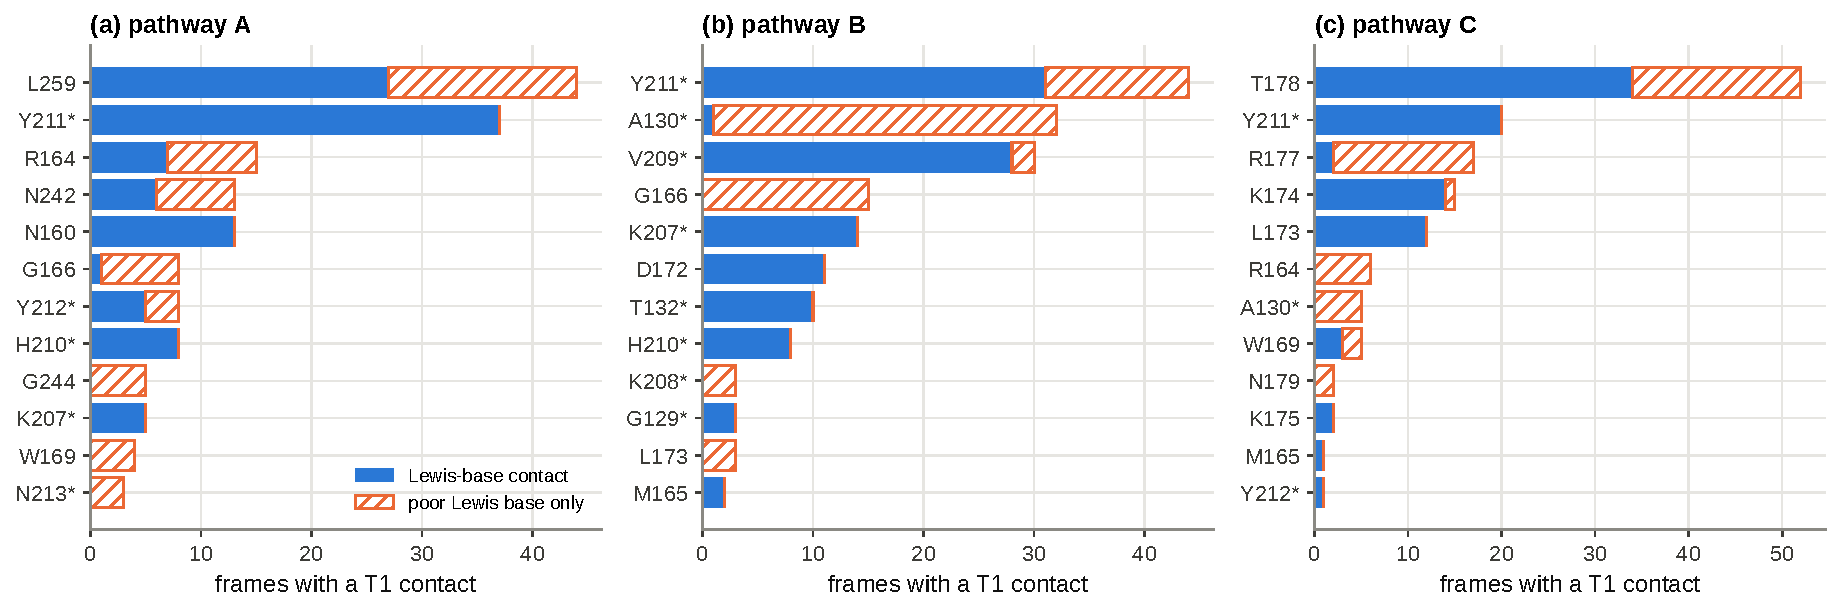
\includegraphics[width=0.85\textwidth]{FigS7_hiyd_residues.pdf}
\caption{Residues with T1 contacts to the iodine of I-Tyr (all 25-ns frames). Blue: frames with a Lewis-base contact. Hatched: frames with contacts to poor Lewis bases only. $^{*}$Chain B.}
\label{fig:hiydres}
\end{figure}

\paragraph{NBO.} A second parser assigned every LP$\to\sigma^*$(C--I) term to the intramolecular or the intermolecular class, and both parsers agree for all 56 outputs. Table~\ref{tab:hiydnbo} and Figure~\ref{fig:hiydnbo} give the terms. All 18 published models with a backbone N acceptor contain the N with one heavy-atom neighbour (C$_\alpha$) and two hydrogens, that is, an amine. Set K rebuilds the hydrogen that replaced the preceding carbonyl carbon as an acetyl group, C(=O)CH$_3$, and keeps everything else of the published input, including the pose, the C-terminal cap, and the level. With the amide restored, none of the 18 poses is supported (five inconclusive, 0.33--0.79~kcal\,mol$^{-1}$, and 13 not supported); the five poses supported as amines (W169, H167, F201$^*$, A130$^*$ in pathway C, and T178; 0.81--1.63~kcal\,mol$^{-1}$) give 0.00--0.79~kcal\,mol$^{-1}$, and eight poses show a dominant N--H$\cdots$I hydrogen bond (0.97--4.60~kcal\,mol$^{-1}$). The A130$^*$ job of pathway C stopped while writing the NBO file after the complete NBO analysis had been printed, and its values are used. Over all 56 poses, with the acetyl-capped values for backbone N, 8 are supported, 19 inconclusive, and 29 not supported; the FMN N5 pose is supported (1.95~kcal\,mol$^{-1}$) but flagged, because the I$\to\sigma^*$(N5--H) donation is 5.65~kcal\,mol$^{-1}$.

\begin{figure}[!htbp]
\centering
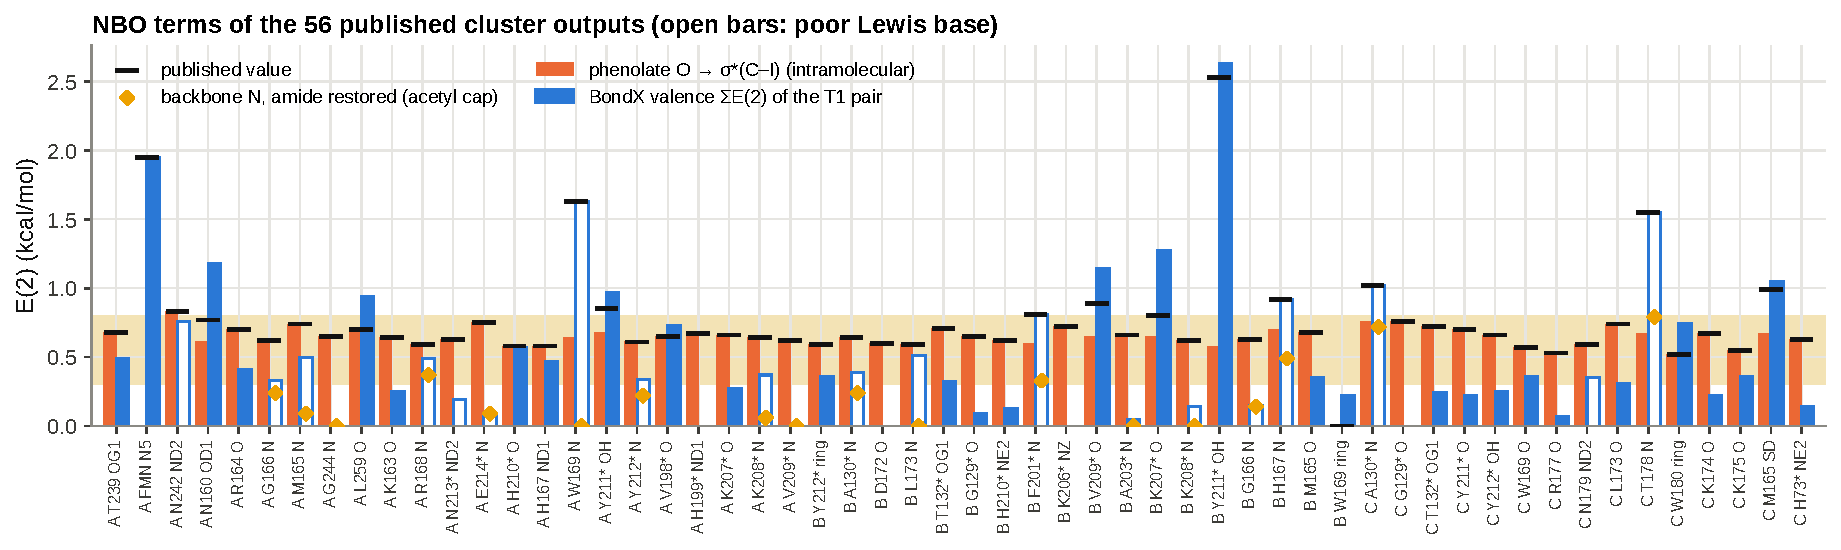
\includegraphics[width=\textwidth]{FigS8_hiyd_nbo.pdf}
\caption{NBO terms of the 56 published cluster outputs. Orange: phenolate O of I-Tyr $\to\sigma^*$(C--I) (intramolecular). Blue: \BX{} valence $\Sigma\ET$ of the T1 pair; open bars: poor Lewis base in the protein (amine in the published model). Black tick: published value. Shaded band: grey zone.}
\label{fig:hiydnbo}
\end{figure}

% ---- table from tables/tab_hiyd_nbo.tex (generated) ----
{\scriptsize
\setlength{\tabcolsep}{3pt}
\begin{longtable}{llrllrrrrrlrrl}
\caption{NBO screen of the 56 published hIYD poses (B3LYP-D3/6-311++G(d,p) with LANL2DZdp on I, CPCM $\varepsilon=4$; kcal\,mol$^{-1}$).\cite{Karmakar2026} $\xi$: window (\AA). $d$ (\AA) and $\theta_1$ ($^\circ$): T1 geometry of the published pose. Base: Lewis class of the acceptor in the protein (poor: delocalized or protonated lone pair). Pub.: published value. Intra: lone pair of the phenolate O of I-Tyr into $\sigma^*$(C--I) of the same ring. $\Sigma E^{(2)}$ and D: valence decision value and decision for the published model; all 18 backbone N acceptors of the published models are amines, because a hydrogen replaced the preceding carbonyl carbon. cap: valence value after this hydrogen was rebuilt as an acetyl group (set K; same pose and level). X$\to$Y--H: halogen lone pairs into N--H or O--H antibonds (for backbone N, of the acetyl-capped model). Final: decision with the acetyl-capped models for backbone N; $^\dagger$: the competing hydrogen bond to I exceeds $\Sigma E^{(2)}$. One set-K job (A130$^*$, pathway C) stopped while writing the NBO file after the complete NBO analysis had been printed; its values are used. These outputs use a different level of theory from the one the grey zone was derived for.}\label{tab:hiydnbo}\\
\toprule
Path & Residue & $\xi$ & Y & Base & $d$ & $\theta_1$ & Pub. & Intra & $\Sigma E^{(2)}$ & D & cap & X$\to$Y--H & Final\\
\midrule
\endfirsthead
\toprule
Path & Residue & $\xi$ & Y & Base & $d$ & $\theta_1$ & Pub. & Intra & $\Sigma E^{(2)}$ & D & cap & X$\to$Y--H & Final\\
\midrule
\endhead
\bottomrule
\endlastfoot
A & T239 & 7.2 & OG1 & base & 3.51 & 149.0 & 0.68 & 0.68 & 0.49 & I &  & 0.00 & I\\
A & FMN & 8.6 & N5 & base & 3.19 & 143.1 & 1.95 & 0.00 & 1.95 & S &  & 5.65 & S$^\dagger$\\
A & N242 & 11.8 & ND2 & poor & 3.51 & 173.1 & 0.83 & 0.83 & 0.76 & I &  & 0.25 & I\\
A & N160 & 12.8 & OD1 & base & 3.35 & 174.9 & 0.77 & 0.61 & 1.18 & S &  & 0.00 & S\\
A & R164 & 13.8 & O & base & 3.55 & 178.3 & 0.70 & 0.70 & 0.41 & I &  & 0.00 & I\\
A & G166 & 13.8 & N & poor & 3.62 & 169.9 & 0.62 & 0.62 & 0.33 & I & 0.24 & 2.28 & N$^\dagger$\\
A & M165 & 15.8 & N & poor & 3.84 & 177.6 & 0.74 & 0.74 & 0.50 & I & 0.09 & 0.00 & N\\
A & G244 & 16.8 & N & poor & 3.47 & 164.8 & 0.65 & 0.65 & 0.00 & N & 0.00 & 4.20 & N$^\dagger$\\
A & L259 & 16.8 & O & base & 3.45 & 173.3 & 0.70 & 0.70 & 0.94 & S &  & 0.00 & S\\
A & K163 & 16.8 & O & base & 3.76 & 156.8 & 0.64 & 0.64 & 0.25 & N &  & 0.00 & N\\
A & R168 & 17.8 & N & poor & 3.49 & 161.5 & 0.59 & 0.59 & 0.49 & I & 0.37 & 4.60 & I$^\dagger$\\
A & N213* & 17.8 & ND2 & poor & 3.94 & 170.0 & 0.63 & 0.63 & 0.19 & N &  & 0.00 & N\\
A & E214* & 17.8 & N & poor & 3.84 & 161.9 & 0.75 & 0.75 & 0.08 & N & 0.09 & 1.66 & N$^\dagger$\\
A & H210* & 17.8 & O & base & 3.26 & 178.5 & 0.58 & 0.58 & 0.57 & I &  & 0.00 & I\\
A & H167 & 17.8 & ND1 & base & 3.67 & 150.3 & 0.58 & 0.58 & 0.47 & I &  & 0.00 & I\\
A & W169 & 17.8 & N & poor & 3.34 & 171.4 & 1.63 & 0.64 & 1.63 & S & 0.00 & 0.33 & N\\
A & Y211* & 17.8 & OH & base & 3.40 & 176.3 & 0.85 & 0.68 & 0.97 & S &  & 0.00 & S\\
A & Y212* & 17.8 & N & poor & 3.65 & 160.9 & 0.61 & 0.61 & 0.34 & I & 0.22 & 2.68 & N$^\dagger$\\
A & V198* & 17.8 & O & base & 3.51 & 172.6 & 0.65 & 0.65 & 0.73 & I &  & 0.00 & I\\
A & H199* & 18.8 & ND1 & base & 3.78 & 145.8 & 0.67 & 0.67 & 0.00 & N &  & 0.00 & N\\
A & K207* & 18.8 & O & base & 3.72 & 178.7 & 0.66 & 0.66 & 0.27 & N &  & 0.00 & N\\
A & K208* & 18.8 & N & poor & 3.82 & 150.1 & 0.64 & 0.64 & 0.37 & I & 0.06 & 0.00 & N\\
A & V209* & 18.8 & N & poor & 3.76 & 166.3 & 0.62 & 0.62 & 0.00 & N & 0.00 & 1.75 & N$^\dagger$\\
B & Y212* & 8.2 & ring & base & 3.93 & 142.6 & 0.59 & 0.59 & 0.36 & I &  & 0.00 & I\\
B & A130* & 9.8 & N & poor & 3.93 & 173.2 & 0.64 & 0.64 & 0.39 & I & 0.24 & 0.00 & N\\
B & D172 & 10.8 & O & base & 3.69 & 160.5 & 0.60 & 0.60 & 0.00 & N &  & 0.00 & N\\
B & L173 & 10.8 & N & poor & 3.69 & 144.1 & 0.59 & 0.59 & 0.51 & I & 0.00 & 0.00 & N\\
B & T132* & 10.8 & OG1 & base & 3.76 & 162.2 & 0.71 & 0.71 & 0.32 & I &  & 0.05 & I\\
B & G129* & 12.8 & O & base & 3.57 & 154.0 & 0.65 & 0.65 & 0.09 & N &  & 0.00 & N\\
B & H210* & 13.8 & NE2 & base & 3.87 & 178.0 & 0.62 & 0.62 & 0.13 & N &  & 0.00 & N\\
B & F201* & 13.8 & N & poor & 3.65 & 159.1 & 0.81 & 0.60 & 0.81 & S & 0.33 & 0.00 & I\\
B & K206* & 14.8 & NZ & poor & 3.80 & 157.7 & 0.72 & 0.72 & 0.00 & N &  & 0.31 & N\\
B & V209* & 15.8 & O & base & 3.22 & 177.6 & 0.89 & 0.65 & 1.14 & S &  & 0.00 & S\\
B & A203* & 16.8 & N & poor & 3.79 & 148.5 & 0.66 & 0.66 & 0.05 & N & 0.00 & 4.16 & N$^\dagger$\\
B & K207* & 16.8 & O & base & 3.20 & 178.3 & 0.80 & 0.65 & 1.27 & S &  & 0.00 & S\\
B & K208* & 16.8 & N & poor & 3.91 & 153.8 & 0.62 & 0.62 & 0.14 & N & 0.00 & 0.00 & N\\
B & Y211* & 16.8 & OH & base & 3.13 & 177.0 & 2.53 & 0.58 & 2.63 & S &  & 0.00 & S\\
B & G166 & 17.8 & N & poor & 3.68 & 178.4 & 0.63 & 0.63 & 0.15 & N & 0.14 & 0.15 & N\\
B & H167 & 17.8 & N & poor & 3.58 & 156.5 & 0.92 & 0.70 & 0.92 & S & 0.49 & 0.08 & I\\
B & M165 & 17.8 & O & base & 3.70 & 167.0 & 0.68 & 0.68 & 0.35 & I &  & 0.00 & I\\
B & W169 & 18.8 & ring & base & 3.91 & 151.6 & 0.00 & 0.00 & 0.22 & N &  & 0.00 & N\\
C & A130* & 8.8 & N & poor & 3.41 & 175.9 & 1.02 & 0.76 & 1.02 & S & 0.72 & 0.97 & I$^\dagger$\\
C & G129* & 8.8 & O & base & 3.73 & 170.1 & 0.76 & 0.76 & 0.00 & N &  & 0.00 & N\\
C & T132* & 8.8 & OG1 & base & 3.81 & 161.5 & 0.72 & 0.72 & 0.24 & N &  & 0.11 & N\\
C & Y211* & 8.8 & O & base & 3.51 & 178.2 & 0.70 & 0.70 & 0.22 & N &  & 0.00 & N\\
C & Y212* & 9.8 & OH & base & 3.48 & 167.4 & 0.66 & 0.66 & 0.25 & N &  & 1.97 & N$^\dagger$\\
C & W169 & 11.8 & O & base & 3.82 & 175.3 & 0.57 & 0.57 & 0.36 & I &  & 0.00 & I\\
C & R177 & 15.8 & O & base & 3.66 & 178.7 & 0.53 & 0.53 & 0.07 & N &  & 0.00 & N\\
C & N179 & 15.8 & ND2 & poor & 3.68 & 169.1 & 0.59 & 0.59 & 0.35 & I &  & 0.00 & I\\
C & L173 & 15.8 & O & base & 3.57 & 170.5 & 0.74 & 0.74 & 0.31 & I &  & 0.00 & I\\
C & T178 & 15.8 & N & poor & 3.53 & 178.1 & 1.55 & 0.67 & 1.55 & S & 0.79 & 0.00 & I\\
C & W180 & 15.8 & ring & base & 3.62 & 154.3 & 0.52 & 0.52 & 0.74 & I &  & 0.00 & I\\
C & K174 & 16.8 & O & base & 3.64 & 176.8 & 0.67 & 0.67 & 0.22 & N &  & 0.00 & N\\
C & K175 & 16.8 & O & base & 3.71 & 174.7 & 0.55 & 0.55 & 0.36 & I &  & 0.00 & I\\
C & M165 & 17.8 & SD & base & 3.70 & 169.3 & 0.99 & 0.67 & 1.05 & S &  & 0.00 & S\\
C & H73* & 18.8 & NE2 & base & 3.65 & 167.9 & 0.63 & 0.63 & 0.14 & N &  & 0.00 & N\\
\end{longtable}}
% ---- end of tables/tab_hiyd_nbo.tex ----

\paragraph{Persistence.} Figure~\ref{fig:hiydt2} shows the occupancy and residence time of the 144 window contacts found by tier T2 with the reporting threshold set to zero, and Table~\ref{tab:hiydt5} lists the contacts with the highest occupancy, with the NBO value of the same residue and acceptor atom only where the NBO output comes from the same window. Because the analysed frames are 160--240~ps apart, the residence factor of $D$ is at least $[1-\exp(-1.6)]^{1/4} = 0.95$, so $D$ is practically the occupancy, and 75\% of the contacts do not persist beyond one saved frame; the program reports this whenever the frame spacing reaches $\tau_0$.

\begin{figure}[!htbp]
\centering
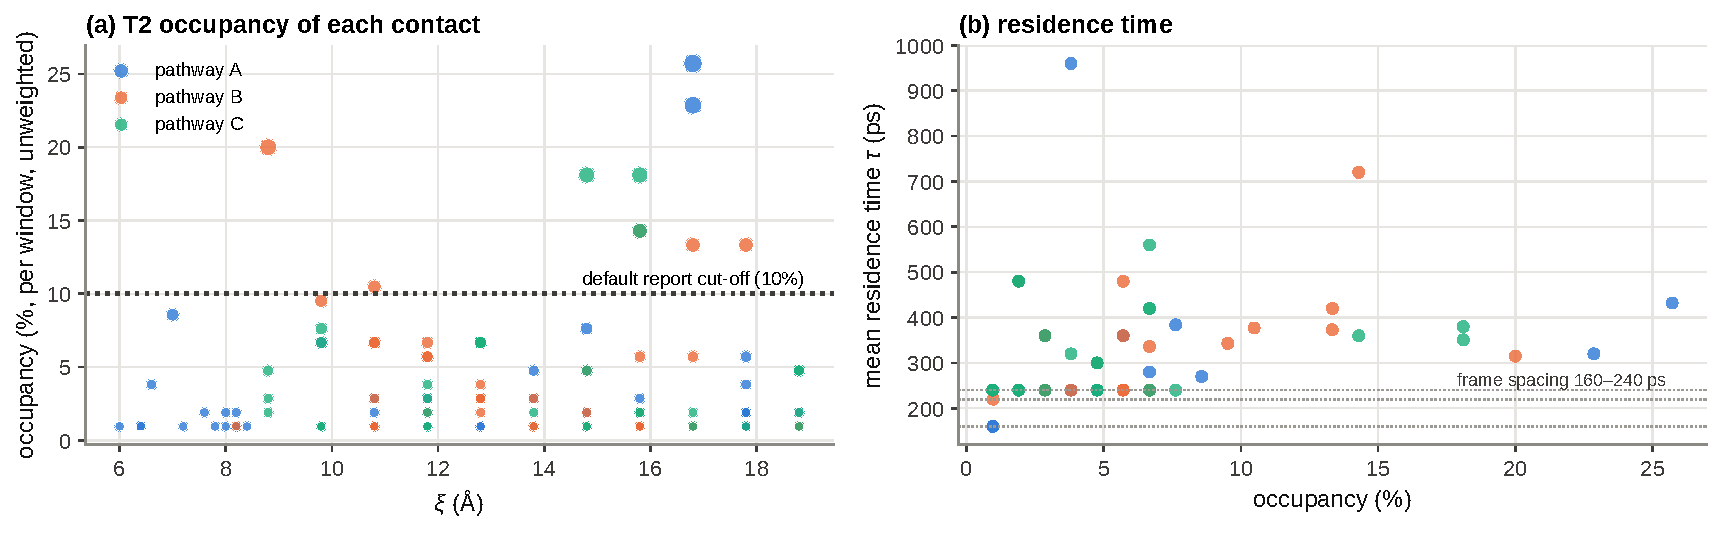
\includegraphics[width=\textwidth]{FigS9_hiyd_T2.pdf}
\caption{Tier T2 on the 108 hIYD windows. (a) Occupancy of each contact in its window (unweighted) against $\xi$; marker size grows with $D$; dotted line: default reporting threshold. (b) Mean residence time against occupancy.}
\label{fig:hiydt2}
\end{figure}

% ---- table from tables/tab_hiydt5.tex (generated) ----
\begin{table}[!htbp]\centering\scriptsize\setlength{\tabcolsep}{3pt}
\caption{Tier T2 on the hIYD release windows for the contacts with the highest occupancy. Occupancy: share of the frames of one umbrella window (unweighted, \%). $\tau$: mean residence time (ps; 20~ps per MD frame times the stride of the stripped file). $D$: persistence score ($\tau_0 = 100$~ps); at the frame spacing of these windows (160--240~ps), $D/f \ge 0.95$, so $D$ is practically the occupancy. $G$: best frame. $\Sigma E^{(2)}$: valence value of the NBO output for the same residue and acceptor atom in the same window (published model; acetyl-capped model for backbone N; ``--'': no output from this window).}\label{tab:hiydt5}
\begin{tabular}{lllrrrrrrr}\toprule Path & Residue & Y & $\xi$ & Occ. & $\tau$ & $D$ & $D/f$ & $G$ & $\Sigma E^{(2)}$\\\midrule
A & L259 & O & 16.8 & 25.7 & 432 & 0.26 & 1.00 & 0.51 & 0.94\\
B & A130* & N & 8.8 & 20.0 & 315 & 0.20 & 0.99 & 0.49 & --\\
C & T178 & N & 15.8 & 18.1 & 380 & 0.18 & 0.99 & 0.55 & 0.79\\
B & V209* & O & 15.8 & 14.3 & 720 & 0.14 & 1.00 & 0.85 & 1.14\\
B & G166 & N & 17.8 & 13.3 & 420 & 0.13 & 1.00 & 0.52 & 0.14\\
B & K207* & O & 16.8 & 13.3 & 373 & 0.13 & 0.99 & 0.71 & 1.27\\
B & D172 & O & 10.8 & 10.5 & 377 & 0.10 & 0.99 & 0.58 & 0.00\\
A & N160 & OD1 & 14.8 & 7.6 & 384 & 0.08 & 0.99 & 0.79 & --\\
C & L173 & O & 12.8 & 6.7 & 560 & 0.07 & 1.00 & 0.56 & --\\
C & K174 & O & 12.8 & 6.7 & 420 & 0.07 & 1.00 & 0.49 & --\\
B & Y211* & OH & 15.8 & 5.7 & 480 & 0.06 & 1.00 & 0.70 & --\\
B & T132* & OG1 & 11.8 & 5.7 & 240 & 0.06 & 0.98 & 0.34 & --\\
A & G244 & N & 14.8 & 4.8 & 300 & 0.05 & 0.99 & 0.49 & --\\
C & A130* & N & 8.8 & 4.8 & 300 & 0.05 & 0.99 & 0.34 & 0.72\\
A & G166 & N & 13.8 & 4.8 & 240 & 0.05 & 0.98 & 0.35 & 0.24\\
A & K207* & O & 18.8 & 4.8 & 240 & 0.05 & 0.98 & 0.92 & 0.27\\
A & Y211* & OH & 17.8 & 3.8 & 960 & 0.04 & 1.00 & 0.76 & 0.97\\
C & Y211* & O & 8.8 & 2.9 & 240 & 0.03 & 0.98 & 0.27 & 0.22\\
B & L173 & N & 10.8 & 2.9 & 240 & 0.03 & 0.98 & 0.22 & 0.00\\
A & R164 & O & 13.8 & 2.9 & 240 & 0.03 & 0.98 & 0.76 & 0.41\\
A & N242 & ND2 & 10.8 & 2.9 & 240 & 0.03 & 0.98 & 0.28 & --\\
B & G129* & O & 12.8 & 2.9 & 240 & 0.03 & 0.98 & 0.22 & 0.09\\
B & M165 & O & 15.8 & 1.9 & 480 & 0.02 & 1.00 & 0.45 & --\\
C & K175 & O & 16.8 & 1.9 & 480 & 0.02 & 1.00 & 0.77 & 0.36\\
A & N213* & ND2 & 17.8 & 1.9 & 240 & 0.02 & 0.98 & 0.46 & 0.19\\
C & N179 & ND2 & 13.8 & 1.9 & 240 & 0.02 & 0.98 & 0.26 & --\\
C & R177 & O & 15.8 & 1.9 & 240 & 0.02 & 0.98 & 0.34 & 0.07\\
A & M165 & N & 15.8 & 1.9 & 240 & 0.02 & 0.98 & 0.42 & 0.09\\
A & R168 & N & 17.8 & 1.9 & 240 & 0.02 & 0.98 & 0.47 & 0.37\\
A & V198* & O & 17.8 & 1.9 & 240 & 0.02 & 0.98 & 0.55 & 0.73\\
A & W169 & N & 18.8 & 0.9 & 240 & 0.01 & 0.98 & 0.20 & --\\
A & FMN & N5 & 8.2 & 0.9 & 240 & 0.01 & 0.98 & 0.22 & --\\
A & Y212* & N & 18.8 & 0.9 & 240 & 0.01 & 0.98 & 0.56 & --\\
B & A203* & N & 13.8 & 0.9 & 240 & 0.01 & 0.98 & 0.29 & --\\
B & K208* & N & 16.8 & 0.9 & 240 & 0.01 & 0.98 & 0.14 & 0.00\\
C & W169 & O & 11.8 & 0.9 & 240 & 0.01 & 0.98 & 0.54 & 0.36\\
C & M165 & SD & 17.8 & 0.9 & 240 & 0.01 & 0.98 & 0.24 & 1.05\\
C & Y212* & OH & 9.8 & 0.9 & 240 & 0.01 & 0.98 & 0.45 & 0.25\\
A & T239 & OG1 & 6.4 & 1.0 & 160 & 0.01 & 0.95 & 0.20 & --\\
\bottomrule\end{tabular}\end{table}
% ---- end of tables/tab_hiydt5.tex ----

%% =====================================================================
\section{Software, Scripts, and Reproducibility}
\label{sec:tests}

% Original test-count and pipeline-repeatability description retained for reference.
% The engine has 120 automated tests (Table~\ref{tab:tests}). A browser test visits every page, including the tutorial; it screens three test-set proteins on the batch page, which give the expected 7, 2, and 2 contacts, and it reads a small CIF on the crystal page, finds the expected I$\cdots$N contact, and builds its QM model. Figure~\ref{fig:perf} and Table~\ref{tab:perf} give the timings, and Table~\ref{tab:scripts} lists the scripts. The full pipeline (\texttt{run\_pipeline.sh}) ran three times in fresh folders, and all result files agree except the timing columns. The analysis steps of \BX{} (\texttt{run\_pipeline\_v3.sh}: scripts 18--21, 27, 28, 11, and 26) also ran three times in fresh folders with the current engine, and every file in \texttt{results/v3/} and \texttt{tables/} was identical in all runs.
\tcb{The engine has 123 automated tests (Table~\ref{tab:tests}), including regression tests for the carbon-bound Cl/Br/I donor definition and the hybridization-dependent $\theta_2$ score; all 123 pass. The independent force-field reference comparisons also pass. A browser test visits every page, including the tutorial, and verifies the expected batch and crystal examples. After the T1 implementation changes, the HAL59 T1 benchmark, paper figure-generation script, and manuscript/ESI table-generation scripts were rerun with the updated engine. The complete end-to-end paper pipeline was not rerun after these changes; analyses outside the regenerated T1-dependent outputs retain their previously archived results.}


% ---- table from tables/tab_tests.tex (generated) ----
{\scriptsize
\setlength{\tabcolsep}{3pt}
\begin{longtable}{rp{14.5cm}}
\caption{The 123 automated engine tests (\texttt{node tests/engine.test.js}). The last test runs the independent force-field comparison listed in Table~\ref{tab:ffref}.}\label{tab:tests}\\
\toprule
\# & Automated test (all passed)\\
\midrule
\endfirsthead
\toprule
\# & Automated test (all passed)\\
\midrule
\endhead
\bottomrule
\endlastfoot
1 & every documented parameter exists in DEFAULTS\\
2 & assumptions listed for T0\\
3 & assumptions listed for T1\\
4 & assumptions listed for T2\\
5 & assumptions listed for T3\\
6 & assumptions listed for T3b\\
7 & assumptions listed for T4\\
8 & assumptions listed for T5\\
9 & QM/MM assumptions mention boundary scheme\\
10 & deep merge changes one value only\\
11 & ff14SB: atom charges of all 110 residue templates sum to the template net charge\\
12 & ff19SB: atom charges of all 110 residue templates sum to the template net charge\\
13 & charmm36: atom charges of all 105 residue templates sum to the template net charge\\
14 & ff14SB: net charges of titratable variants and termini\\
15 & charmm36: net charges of titratable variants and termini\\
16 & ff14SB backbone charges (Cornell et al.)\\
17 & CHARMM36 backbone charges\\
18 & TIP3P water\\
19 & I$\cdots$O=C backbone XB found\\
20 & Br$\cdots\pi$(Phe) XB found\\
21 & G worked example = 0.859 (ESI S4)\\
22 & changing a cut-off changes detection\\
23 & cut-off above 4.6 \AA{} is honoured (search radius follows cut-offs)\\
24 & D worked example = 0.586 ($\tau$ = 160 ps, $\tau$0 = 100 ps)\\
25 & T1 donor list excludes non-C-bound Br$\cdots$Br and retains C-bound I\\
26 & linear nitrile N uses sp-specific $\theta_2$ optimum of 180$^\circ$\\
27 & hybridization-specific $\theta_2$ scoring corrects the old sp-nitrile penalty\\
28 & chain termini detected\\
29 & terminal templates NALA / CGLY used\\
30 & demo peptide net charge $-$1 (NH3+, Asp$-$, COO$-$) with folded H: -1.000000\\
31 & water without H is neutral (H folded)\\
32 & CHARMM36 gives the same net charge\\
33 & neutral termini option runs\\
34 & per-residue override ASP$\to$ASH\\
35 & hbShell: residues with N--H/O--H near X join fragment 2 and are reported (25 $\to$ 41 atoms)\\
36 & fragment charges from templates (ligand 0, N-terminal Ala +1): \{"1":0,"2":1\}\\
37 & Ala: 3 H on N-terminal N, 1 on CA, 3 on CB (from NALA template)\\
38 & even electron count\\
39 & no atoms closer than 0.9 \AA{} in the QM model: 1.010\\
40 & manifest records residue charges, assumptions, and force field\\
41 & scaled link-atom scheme builds the same topology\\
42 & IDD594 Br$\cdots$OG1 Thr113 detected at 2.97 \AA{}\\
43 & 1US0 protein: summed atom charges (0.0000) equal the sum of template charges (0)\\
44 & 1US0 net charge = Arg+Lys$-$Asp$-$Glu+termini (0)\\
45 & Thr113 cluster: fragment charges \{"1":-1,"2":0\}, even electrons\\
46 & Thr: H on N, CA, CB, and OG1 and 3 on CG2 (from THR template)\\
47 & Thr113 OG1-H rotamer: best 3.48 \AA{}, toward Br 2.61 \AA{}, away 3.48 \AA{} from Br\\
48 & competing H-bond flag when X$\to\sigma$*(O--H) (2.00) exceeds $\Sigma$E(2) (1.00): hbond\\
49 & poor Lewis base flag kept, no H-bond flag below $\Sigma$E(2): poorBase\\
50 & a supported contact with a dominant competing H-bond ranks after a clean supported contact\\
51 & warning when the frame spacing is not shorter than $\tau$0\\
52 & D(f = 0.257, $\tau$ = 160 ps) = 0.243 $\approx$ f\\
53 & RC boundary conserves the MM charge exactly (0.000000)\\
54 & whole-residue embedding carries an integer net charge\\
55 & Z1 deletes the 2 M1 charges\\
56 & side-chain QM: cut-residue correction gives integer MM charge (-0.0000 vs -0.1144 uncorrected)\\
57 & RCD boundary conserves the MM charge (0.000000)\\
58 & explicit MM hydrogens near X (72) keep the net charge\\
59 & zero-charge MM atoms are counted\\
60 & backbone N acceptor keeps its amide (36 $\to$ 50 atoms)\\
61 & amide N flagged as a poor Lewis base (delocalized)\\
62 & aliphatic amine flagged, or protonated on request\\
63 & N-methylpyridinium: +1 and 8 H\\
64 & short contacts (R $<$ 0.80) flagged\\
65 & optional short-contact penalty\\
66 & anionic model without diffuse functions gets a caution\\
67 & Thr113 hydroxyl H: 2.20 \AA{} from Br with the fixed rule, 3.48 \AA{} after orientation\\
68 & Gaussian input: charge keyword and point-charge block\\
69 & ORCA .pc file: count line\\
70 & Q-Chem \$external\_charges block\\
71 & charges CSV export\\
72 & auto charge source uses PQR charges when a PQR is loaded\\
73 & MOL2 without charges is rejected with an explanation\\
74 & MOL2 charges read (PRODRG acetate: CAB 0.72, total 0)\\
75 & manifest geometry verified against output\\
76 & $\Sigma$E(2) with RY* = 3.68\\
77 & $\Sigma$E(2) without RY* = 3.47 (option)\\
78 & raising the upper grey-zone limit makes 3.47 inconclusive\\
79 & valence decision value with the Rydberg part reported beside it\\
80 & grey zone 0.3--0.8 kcal/mol\\
81 & Rydberg terms are off in the default decision\\
82 & output with different atom count is refused\\
83 & EDA summary parsed and converted to kcal/mol\\
84 & kcal/mol output kept\\
85 & $\chi$\_CT = 0.66 $\to$ CT driven\\
86 & changing $\chi$\_CT threshold changes the label\\
87 & BXQI worked example = 64.6, no grades\\
88 & unevaluable tier is dropped, not floored\\
89 & repulsive EDA total gives s\_C = 0\\
90 & EDA tier can be switched off\\
91 & ranking follows the NBO decision first\\
92 & DCD and multi-model PDB give the same persistence\\
93 & D uses the documented formula with $\tau$ in ps\\
94 & CIF I$\cdots$N found\\
95 & symmetry-equivalent CIF contacts reported once (2 copies)\\
96 & unsafe CIF symmetry operator refused\\
97 & altloc: first conformer kept by default\\
98 & altloc: highest-occupancy option\\
99 & cryo-EM 1 \AA{} dummy cell is ignored (no false periodic contacts)\\
100 & Gaussian: D3(BJ) only for hybrids without built-in dispersion\\
101 & ORCA: dispersion keyword chosen per functional\\
102 & ORCA NBO caution in input comments and T3 assumptions\\
103 & Q-Chem: DFT\_D D3\_BJ written when requested\\
104 & strong XB contact is never used to join the two fragments\\
105 & polar-H-only input: C--H completed, same 50-atom model as from the H-free file\\
106 & 1P5E TBS: C6HBr4N3 with one N-H (got BR4C6H1N3, 1 N-H)\\
107 & 2W0S BVP: phosphate dianion C11H12BrN2O8P, charge -2 (got BR1C11H12N2O8P1, -2)\\
108 & 4GQL R47: incomplete file H rebuilt to 32 H at charge -3 (got 32, -3)\\
109 & 4AGL P84: incomplete ligand (13 of 21 heavy atoms) is reported\\
110 & PDB FORMUL records parsed (formula and charge)\\
111 & replaced file H never become MM charges (4GQL: 1780,2 vs re-protonated 1780,2)\\
112 & added ligand H atoms have no clashes (H-H $>$= 1.2 A, H-X $>$= 1.5 A; 0 found)\\
113 & extra point EP of I-Tyr removed on reading (1 site, 2644 of 2645 atoms kept)\\
114 & iodine partner is the ring carbon C6, not the extra point\\
115 & DCD/XYZ frames written with the extra point are mapped to the kept atoms\\
116 & frames with a wrong atom count are refused\\
117 & NBO lines with an orbital index above 999 (printed ***) are read\\
118 & Q-Chem NBO input requests the E(2) table and uses the Q-Chem 6 PCM keyword Dielectric\\
119 & Q-Chem NBO input with def2-QZVP carries the pure-g caution\\
120 & Q-Chem NBO caution in the T3 assumptions\\
121 & ionic NBO structure (vacant LP* on the halogen, no sigma*(A-X)) counts n -$>$ LP*(X)\\
122 & LP*(X) is ignored when the sigma*(A-X) orbital exists\\
123 & force-field charges agree with PDB2PQR reference PQR files\\
\end{longtable}}
% ---- end of tables/tab_tests.tex ----

\begin{figure}[!htbp]
\centering
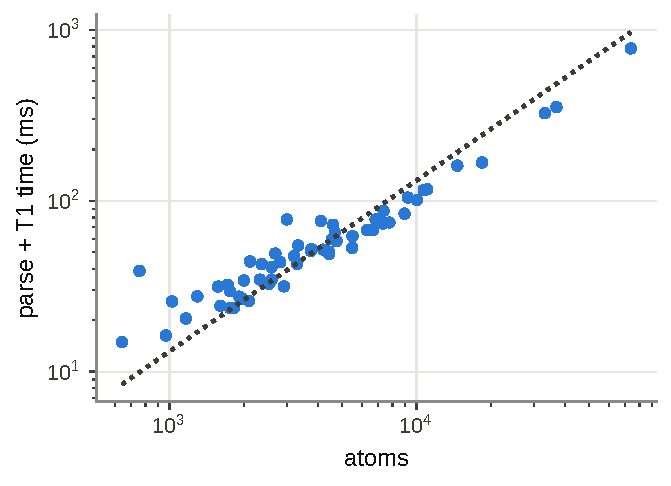
\includegraphics[width=0.45\textwidth]{FigS10_performance.pdf}
\caption{Parse and T1 detection time against the number of atoms. Dotted line: linear scaling.}
\label{fig:perf}
\end{figure}

% ---- table from tables/tab_performance.tex (generated) ----
\begin{table}[!htbp]\centering\footnotesize
\caption{Run time of the \BX{} engine (Node.js 22, one core of an Intel Xeon at 2.3 GHz, median of five runs). Times include file parsing.}\label{tab:perf}
\begin{tabular}{lrl}\toprule Task & Atoms & Time (ms)\\\midrule
T1 detection, 56 test structures & 643--33072 & 15--325 (median 50)\\
T1 detection, 1P5E $\times$ 2 & 18424 & 168\\
T1 detection, 1P5E $\times$ 4 & 36848 & 354\\
T1 detection, 1P5E $\times$ 8 & 73696 & 780\\
T2, 200 frames, 1US0 & 2526 & 13 (15082 frames/s)\\
T2, 200 frames, 1P5E & 9212 & 192 (1039 frames/s)\\
cluster model, 1US0 &  & 46\\
QM/MM model, 1US0 &  & 64\\
cluster model, 1P5E &  & 125\\
QM/MM model, 1P5E &  & 206\\
cluster model, 4GQL &  & 52\\
QM/MM model, 4GQL &  & 72\\
\bottomrule\end{tabular}\end{table}
% ---- end of tables/tab_performance.tex ----

\begin{table}[!htbp]
\caption{Scripts of this work (folder \texttt{Scripts/})}
\label{tab:scripts}
\centering\footnotesize
\begin{tabularx}{\textwidth}{@{}>{\raggedright\arraybackslash}p{5.4cm}>{\raggedright\arraybackslash}X@{}}
\toprule
File & Task \\
\midrule
\texttt{engine.js}, \texttt{ff\_data.js}, \texttt{bondx\_cli.js} & The \BX{} engine, force-field tables, and command-line front end \\
\texttt{bxutil.py}, \texttt{bxstyle3.py} & Shared helpers and figure style (Arial, no legend frames) \\
\texttt{00}--\texttt{02} & PubMed counts; HAL59 geometries; rigid scans \\
\texttt{03}, \texttt{06} & Tier T1 on HAL59 and scans; T1 parameter grid \\
\texttt{04}, \texttt{05} & QM inputs of sets A--E; protein T1, 89 QM models, and set F inputs \\
\texttt{07} & Reads all QM outputs with the \BX{} parsers \\
\texttt{09}, \texttt{11}, \texttt{12} & Timings; tables that did not change; Figure~\ref{M-fig:model} \\
\texttt{13}, \texttt{14} & ORCA counterpoise analysis; ligand check against the FORMUL records \\
\texttt{15}, \texttt{16} & hIYD analysis (with \texttt{hiyd\_bondx.js} and \texttt{hiyd\_nbo.js}); hIYD tables \\
\texttt{17} & NBO, ALMO-EDA, and protein analysis with the Rydberg terms counted (superseded by script 18; kept for the EDA and counterpoise columns) \\
\texttt{18} & Re-reads all NBO outputs of sets A--F with the screen of \BX{} (valence part, RY part, X$\to\sigma^*$(Y--H), in-cluster pairs, and amide N atoms) \\
\texttt{19}, \texttt{20} & MM field tests (explicit H, RCD, radius, force field); tier T2 on the hIYD windows \\
\texttt{21} & Statistics with bootstrap intervals, grey zone, BXQI, field versus $\Sigma\ET$, and hIYD T5 \\
\texttt{22}, \texttt{24}, \texttt{25} & Figures~\ref{M-fig:t1}--\ref{M-fig:hiyd}, S1--S10, and S12; interface figures; TOC graphic \\
\texttt{23} & Screenshots of the application (Playwright) \\
\texttt{26} & ESI tables of the NBO screen, the field tests, the job sets G, J, and K, and hIYD \\
\texttt{27} & Sets G, J, and K: the screen of \BX{} (\texttt{27\_v3\_extra\_nbo.js}) and an independent parser without \BX{} code (\texttt{27\_extra\_parse.py}) \\
\texttt{28} & Acceptor classes, grey-zone extremes, competing-hydrogen-bond flags, updated hIYD decisions, and the residence factor of $D$ \\
\texttt{inline\_tables.py} & Writes the tables into \texttt{ESI\_V3.tex} \\
\texttt{run\_pipeline.sh}, \texttt{run\_pipeline\_v3.sh}, \texttt{compare\_runs.py} & Full run and the analysis steps 18--28 in a fresh folder; comparison of two runs \\
\texttt{BondX\_paper\_scripts.ipynb} & All Python scripts of this table in one Jupyter notebook \\
\bottomrule
\end{tabularx}
\end{table}

%% =====================================================================
\section{User Guide}
\label{sec:guide}

Open \url{https://compchemsk.github.io/BondX-Studio/} or the file \texttt{index.html}. The \emph{Tutorial} button opens a guide.
\begin{enumerate}
\item Tier T0: load a PDB or PQR file, a PDB ID, or the demo, and keep the chains you need.
\item Tier T1: run the detection and send the chosen contacts to the registry.
\item Tier T2 (optional): load a topology and a trajectory, set the time between saved frames, and send the best frames to the registry.
\item Tier T3a: choose a cluster or QM/MM model, the force field, and the QM level, check the warnings, and download the job bundle.
\item Tier T3b: run the NBO job, drop the output, and read the decision with its Rydberg part and the competing hydrogen-bond donation.
\item Tier T4: run the EDA job in Q-Chem, drop the output, and read $\chi_\mathrm{CT}$.
\item Tier T5: read the ranking and download the HTML report and the run record.
\end{enumerate}

\begin{figure}[!htbp]
\centering
\includegraphics[width=0.9\textwidth,height=0.75\textheight,keepaspectratio]{FigS11_screens.pdf}
\caption{Tier pages for the demo complex. The NBO and EDA pages read the synthetic example outputs of the program, which only demonstrate the pages.}
\label{fig:screens}
\end{figure}

\FloatBarrier
\bibliography{References_V3}
\end{singlespace}
\end{document}
